\documentclass[a4paper, 12pt]{book}
\includeonly{gis-pfc-pro, gis-pfc-part1, gis-pfc-part2, gis-pfc-ch1, %
	gis-pfc-ch2, gis-pfc-ch3, gis-pfc-ch4, gis-pfc-ch5, gis-pfc-appa, %
	gis-pfc-appb}
\usepackage[english, spanish]{babel}
\usepackage[utf8]{inputenc}
\usepackage[T1]{fontenc}
\usepackage[altbullet, nofontinfo]{lucidabr}
\usepackage[format=hang, font=small, labelfont=bf, labelsep=endash, %
	width=.9\textwidth]{caption}
\usepackage[listofformat=subsimple, format=hang, captionskip=10pt, %
	labelfont=footnotesize, textfont={it, footnotesize}]{subfig}
\setcounter{lofdepth}{2}
\usepackage[clearempty]{titlesec}
\usepackage[nottoc]{tocbibind}
\usepackage[spanish]{varioref}
\usepackage[noauto]{chappg}
\usepackage{graphicx}
\usepackage{amsfonts, amsmath, amssymb, calc, color, fancyhdr, hyperref}
\usepackage{ifthen, layouts, listings, rotating, textcase, textcomp}
\usepackage{array, booktabs, tabularx, tabulary, dcolumn, multirow}
\usepackage{threeparttable}
\usepackage[fixlanguage, noisbn]{babelbib}
\usepackage[spanish]{cleveref}
\titleformat{\part}[display]{\centering\huge\bfseries}
	{\partname\ \thepart}{.5\baselineskip}{}
\hypersetup{
	pdftitle=Proceso de adquisición y tratamiento de señales de
	ultrasonidos, pdfauthor=José Ramón Gisbert Valls,
	pdfcreator=Vim 7.2, pdfstartview=FitH, colorlinks=true,
	pdfdisplaydoctitle=true, linkcolor=black, citecolor=black,
	bookmarksopen=true, bookmarksopenlevel=0, urlcolor=black
}
\fancypagestyle{plain}{
	\fancyhf{}
	\renewcommand\headrulewidth{0pt}
}
\fancypagestyle{Number}{
	\fancyhf{}
	\fancyfoot[C]{\bfseries\scshape\thepage}
	\renewcommand\headrulewidth{0pt}
}
\fancypagestyle{number}{
	\fancyhf{}
	\fancyfoot[C]{\sffamily\bfseries\thepage}
	\renewcommand\headrulewidth{0pt}
}
\fancypagestyle{body}{
	\fancyhf{}
	\fancyhead[RO, LE]{\footnotesize\sffamily\bfseries\thepage}
	\fancyhead[LO]{\footnotesize\sffamily\nouppercase{\rightmark}}
	\fancyhead[RE]{\footnotesize\sffamily\nouppercase{\leftmark}}
	\renewcommand\headrulewidth{0.4pt}
	\renewcommand\chaptermark[1]{\markboth{##1}{}}
}
\lstloadlanguages{Matlab}
\lstset{language=Matlab, extendedchars=true, breaklines, captionpos=b,
	morekeywords={addchannel, analoginput, catch, datadqcallback,
	daqfind, daqhwinfo, errordlg, gcbo, getdata, guidata,
	localDaqCallback, peekdata, single_channel, start, stop, strcmpi,
	trigger, try, warning}
	}
\lstdefinestyle{displayed}{float=tpbh, frame=l, tabsize=5,
	framerule=1.2pt, abovecaptionskip=\medskipamount, gobble=4,
	linewidth=.975\textwidth, xleftmargin=.05\textwidth}
\crefname{lstlisting}{fragmento de código}{fragmentos de código}
\crefname{listing}{fragmento de código}{fragmentos de código}
\crefname{subsection}{subapartado}{subapartados}
\crefname{subsubsection}{subapartado}{subapartados}
\graphicspath{{./pictures/}{../pictures/}}
\DeclareCaptionLabelFormat{cont}{#1~#2\alph{ContinuedFloat}}
\captionsetup[ContinuedFloat]{labelformat=cont}
\DeclareCaptionLabelFormat{romanos}{\textbf{(\,\Roman{figure}\,)}}
\DeclareCaptionListFormat{romanos}{\thepart\,.\,\Roman{figure}\,}
\selectbiblanguage{spanish}
\setbtxfallbacklanguage{english}
\setlength\marginparsep{12pt}
\setlength\marginparwidth{\pdfpagewidth - \textwidth - \oddsidemargin -
	2\marginparsep - 1in}
% Convenios tipográficos: siglas (primera vez), siglas, funciones,
% argumentos, propiedades, atributos de propiedades, nombres de canal o
% puerto
\newcommand\psig[1]{\emph{\MakeTextUppercase{#1}}}
\newcommand\sig [1]{\textsc{\MakeTextLowercase{#1}}}
\newcommand\func[1]{\texttt{#1}}
\newcommand\argu[1]{\texttt{#1}}
\newcommand\prop[1]{\textsf{#1}}
\newcommand\atr [1]{\textsf{#1}}
\newcommand\can [1]{\sig{#1}}
% Palabras predefinidas
\newcommand\matlab{\sig{MATLAB}}
\newcommand\kpci  {\sig{KPCI}-3108}
\newcommand\datx  {\sig{DAT}}
\newcommand\gui   {\sig{GUI}}
\newcommand\guide {\sig{GUIDE}}
\newcommand\pc    {\sig{pc}}
\newcommand\ram   {\sig{ram}}
\newcommand\AOUA  {\ensuremath{\mu}\sig{a}741}
\newcommand\kms   {kmus/s}
\newcommand\miniit[1]{\begin{itemize} #1 \end{itemize}}
\newcommand\tnotetext[2]{\item\hspace*{-5pt}\raisebox{.7ex}%
	{\fontsize{7pt}{8.4pt}\selectfont\normalfont #1}{\footnotesize #2}}
\newcommand\prosec{\smallskip\begin{center}%
	\usefont{T1}{hlh}{m}{n}\UseTextSymbol{OMS}{\textasteriskcentered}%
	\quad\UseTextSymbol{OMS}{\textasteriskcentered}\quad%
	\UseTextSymbol{OMS}{\textasteriskcentered}%
	\end{center}\smallskip}
\renewcommand\labelitemi{\textbullet}
\renewcommand\labelitemii{\leavevmode\hbox to 1.1ex
	{\hss\vrule height .8ex width .6ex depth -.2ex\hss}}
\newcommand\longpage[1][1]{\enlargethispage{#1\baselineskip}}
\newcommand\llongpage[1][0]{\enlargethispage*{#1\baselineskip}}
\newcommand\shortpage[1][1]{\enlargethispage{-#1\baselineskip}}
\renewcommand\chappgsep{--}
\makeatletter\renewcommand\@pnumwidth{21.5pt}\makeatother
\newenvironment{TableNotes}{\begin{tablenotes}\vspace{\footnotesep}
	\footnoterule\vspace{.2ex}}{\end{tablenotes}}
\newcolumntype{d}[1]{D{,}{,}{#1}}
\newcolumntype{+}{D{/}{\mbox{\ --\ }}{5}}
\newcounter{totalpages}
\begin{document}

\setuplayouts
\pagestyle{Number}
\frontmatter
\tableofcontents
\listoftables
\listoffigures
\chapter{Pr�logo}

\section*{Justificaci�n}

\subsubsection{Ensayos no destructivos con ultrasonidos}

Es en la pr�ctica habitual en la actualidad emplear los \emph{ensayos no destructivos} (\psig{end}) en controles de calidad efectuados en la industria de manufactura de materiales, principalmente de metales y de compuestos para la construcci�n. Este tipo de ensayos garantizan ---demostrada su efectividad en este tipo de aplicaciones--- la ausencia de defectos internos como fisuras y de otras imperfecciones como alteraciones en la composici�n del producto, que de no superar controles semejantes pueden pasar inadvertidos. Realizando estos controles se impide la salida al mercado de partidas de producto defectuosas que pudiesen comprometer la calidad de productos finales. En este sentido comprobar el estado de un material resulta en un ejercicio de responsabilidad puesto que muchos de los materiales que proceden de esta industria se destinan a la construcci�n de edificios o de medios de transporte como barcos y aviones. De ah� la necesidad de aplicar en los controles de calidad m�todos que proporcionen resultados efectivos y confiables como lo son los obtenidos con los \sig{end}.\par
La ventajas que presentan los ensayos no destructivos frente a otro tipo de ensayos, no s�lo se limitan al hecho de que no es necesario sacrificar parte de la producci�n para evaluar el producto, si no que tambi�n incluyen una evaluaci�n continua y uniforme del material. Esto redunda en materiales de gran calidad cuyas propiedades se mantiene invariables uniformemente a lo largo del producto. Adem�s, otra ventaja de los \sig{end} es que es posible realizar de nuevo el ensayo una vez el producto final se ha terminado o en posteriores revisiones ya que no causa ning�n da�o en el material. Por �ltimo, cabe destacar que los controles de calidad mediante \sig{end} pueden efectuarse durante el mismo proceso de fabricaci�n de forma automatizada lo que supone una reducci�n en los costes.\par
Por su parte, el uso de ultrasonidos en \sig{end} est� muy extendido, esto es en parte debido a los precisos resultados que proporcionan los \emph{ensayos no destructivos mediante ultrasonidos} (\psig{endus}). Empleando transductores de alta frecuencia y gran ancho de banda es posible distinguir defectos en el material de tama�o muy peque�o de forma inequ�voca. A esto debe sum�rsele la sencillez con la que se aplican los \sig{endus} y las ventajas de emplear transductores de peque�o volumen que permiten trabajar con materiales de formas intrincadas e irregulares.\par
Recientemente se est�n empleando los \sig{endus} en campos experimentales con el prop�sito de detectar la presencia de anomal�as en materiales procedentes de la naturaleza. En estos experimentos el procedimiento a seguir es conforme al uso de los controles de calidad que se practican en el �mbito industrial. Conviene, sin embargo, diferenciar el tipo de medio en el que los ensayos son aplicados. Los ensayos realizados habitualmente a nivel industrial eval�an materiales sint�ticos, bien conocidos, mientras que en su lugar, los ensayos experimentales contemplan materiales org�nicos heterog�neos como es en este caso la madera. Es por ello que la eficacia de los \sig{endus} aplicados sobre materiales org�nicos no est� todav�a demostrada.\par
De la singularidad del material el inter�s de las pruebas, inter�s que se ve reforzado por el hecho de que la madera es un medio <<vivo>>, que cambia de muestra a muestra, las condiciones del ensayo var�an incluso para una misma muestra. Es, por tanto, el uso \sig{endus} para la detecci�n de defectos en madera de palmera un tema de inter�s, de actualidad y muy atractivo, hacia el cual orientar el desarrollo de un proyecto fin de carrera.


\subsubsection{Tratamiento digital de se�ales}

El tratamiento digital de se�ales es una de las disciplinas fundamentales que abarca la ingenier�a de telecomunicaciones. Pese a los inconvenientes inherentes al uso de circuiter�a digital (muestreo y errores de cuantificaci�n principalmente) el procesado digital de se�ales ha demostrado ser una herramienta �til y vers�til.\par
Esa versatilidad se sigue de la capacidad del hardware digital de ser programado, o lo que es lo mismo la capacidad de un circuito de alterar su funcionamiento y proporcionar varias funciones de acuerdo con una configuraci�n por software. Virtud que sumada al reciente desarrollo de las tecnolog�as digitales ha propiciado su explotaci�n y el uso extensivo de aplicaciones basadas en circuiter�a digital.\par
La configuraci�n de un sistema digital a partir de una tarjeta de adquisici�n digital, un ordenador y una suite de software matem�tico supone una oportunidad para comprender aspectos del funcionamiento de los sistemas digitales dif�ciles de observar en la teor�a.


\section*{Objetivos del proyecto fin de carrera}\label{sec:goals}

Inicialmente este proyecto persigue completar dos objetivos distintos: la implementaci�n de un sistema de medida a partir de una tarjeta de adquisici�n con interfaz \sig{pci}; y la evaluaci�n de los \sig{endus} como m�todo para la detecci�n de defectos en madera de palmera.\par
Por un lado, se ha llevado a cabo la puesta en funcionamiento de un sistema de medida con el que es posible obtener un conjunto de par�metros de una determinada se�al. Permite observar la forma que presenta la se�al en cada instante, la forma del espectro de la se�al cuando se enmarca en una ventana de una determinada duraci�n temporal, valores instant�neos y valores medios en un determinado intervalo.\par
Por otro lado, se han llevado a cabo una serie de pruebas experimentales en madera de palmera, empleando para ello se�ales ultras�nicas generadas por un transductor, de forma similar a como se hace en los \sig{endus} de car�cter industrial. Posteriormente las muestras se han procesado para averiguar a partir de los datos que informaci�n sobre el medio ---presencia de fisuras internas, presencia de agua en distintos niveles dependiendo de la altura en la que se realiza la prueba o del estado de salud del esp�cimen, o en general cualquier otra informaci�n de utilidad--- puede extraerse en este tipo de ensayos.\par
Existe una relaci�n visible entre ambos objetivos, la pretensi�n inicial consiste en emplear el sistema de medida digital en la realizaci�n de las pruebas. No obstante, pese a todo, durante el transcurso del proyecto ambos objetivos se tratan por separado. Finalmente, la imposibilidad de realizar las pruebas experimentales con el sistema confeccionado (por motivos que se ver�n m�s adelante) ha conducido al uso de un sistema de medida alternativo. Es por este motivo por el cual resulta comprensible la divisi�n de este documento en dos partes, una por cada objetivo diferenciado.


\section*{Estructura del documento}

Como se ha mencionado en el apartado anterior el documento consta de dos partes. Se ha decidido ordenar las partes en orden cronol�gico. Puesto que ha resultado necesario confeccionar el sistema de medida con anterioridad a la realizaci�n de las primeras pruebas ---esto resulta obvio, pues sin este sistema no es posible realizar las mediciones necesarias---, la primera de las partes trata sobre la implementaci�n del sistema digital de medida. La divisi�n de las partes no es, sin embargo, natural por completo, puesto que para dise�ar el instrumento de medida es necesario haber reunido previamente un determinado conocimiento en materia de \sig{endus}. Todo lo relativo a la teor�a de los \sig{endus} y a los resultados de las pruebas se ha reservado para la segunda parte de la memoria.

\begin{itemize}
	\item La primera parte se divide a su vez en cuatro cap�tulos: subsistema de interacci�n con el medio f�sico; subsistema de adquisici�n; subsistema de control y presentaci�n; y resultados, conclusiones y l�neas futuras de trabajo. Los tres primeros cap�tulos responden a una divisi�n funcional del sistema de medida, observando el sistema de medida como una pila de capas en el que cada capa comprende un subsistema que proporciona servicio a los subsistemas por encima de �l y abstrae las capas inferiores, es posible tratar cada subsistema por separado.
		\begin{itemize}
			\item El primer subsistema interact�a directamente con el medio f�sico, comprende el transmisor de ultrasonidos, el receptor y las etapas de acondicionamiento que los preceden. El primer cap�tulo resume las principales caracter�sticas de estos tres elementos y realiza un recorrido por el proceso de dise�o de este subsistema.
			\item El subsistema intermedio transforma la se�al anal�gica que le es entregada por la secci�n de recepci�n en una se�al digital. El n�cleo y el todo de este subsistema es la tarjeta de adquisici�n. El segundo cap�tulo repasa las caracter�sticas t�cnicas clave de este dispositivo, realiza una descripci�n funcional del mismo y reproduce los consejos que el fabricante proporciona en el manual de usuario para su uso correcto.
			\item El �ltimo de los subsistemas, el subsistema de m�s alto nivel, es el subsistema de control y presentaci�n. Este subsistema interviene como interfaz entre el usuario administrador y el resto de capas (el resto del sistema de medida). Como tal es su funci�n traducir la se�al digital que recibe de capas inferiores en informaci�n �til para el usuario, recibir e interpretar los comandos administrados por el supervisor y gestionar el funcionamiento del resto de subsistemas. El cap�tulo tercero de la primera parte hace hincapi� en el dise�o conceptual de este subsistema y proporciona una serie de detalles t�cnicos en relaci�n con el entorno de programaci�n en el que se ha desarrollado.
			\item En el �ltimo de los cap�tulos de la primera parte se exponen las conclusiones extra�das tras poner a prueba el sistema de medida ya terminado. Se comentan posteriormente l�neas futuras de trabajo que persiguen mejorar la funcionalidad del sistema de medida.
		\end{itemize}
	\item La segunda parte est� dividida en tres cap�tulos: fundamentos te�ricos de los \sig{endus}, descripci�n del medio, resultados y conclusiones.
		\begin{itemize}
			\item En el primer cap�tulo se describen de forma superficial los distintos elementos que intervienen en un \sig{endus} desde un punto de vista te�rico. De las distintas t�cnicas existentes para combatir el ruido estructural se dan detalles sobre las t�cnicas de procesado por partici�n del espectro que son las utilizadas en este proyecto.
			\item El segundo cap�tulo trata sobre el medio en el que se realizan las pruebas experimentales, la madera de palmera. Se proporciona una descripci�n te�rica del material de acuerdo con la documentaci�n consultada. Se caracteriza el material para un posterior an�lisis de los resultados encontrados en las pruebas experimentales.
			\item El �ltimo cap�tulo recoge los resultados extra�dos de las pruebas en forma de grafos y tablas comentados. Despu�s se dan las conclusiones a las que se ha llegado a partir de estos resultados y finalmente se realizan una serie de comentarios sobre nuevas l�neas de investigaci�n que pueden seguirse de este proyecto
		\end{itemize}
	\item Dos ap�ndices cierran este documento: el primero es un manual de instrucciones para el uso del sistema de medida, y el segundo es un ap�ndice que muestra detalles sobre este documento.
		\begin{itemize}
			\item El primer ap�ndice proporciona un manual de usuario para el uso de la aplicaci�n de software inform�tico que funciona como subsistema de control del sistema digital de medida implementado para este proyecto. Este contenido se ha extra�do del grueso del documento, pues no concierne al desarrollo del proyecto.
			\item El segundo ap�ndice muestra detalles sobre la memoria como por ejemplo la estructura de sus p�ginas, glosarios, �ndices de contenidos y referencias.
		\end{itemize}
\end{itemize}
% Existe una relaci�n visible entre ambos objetivos, la pretensi�n inicial consiste en emplear el sistema de medida en la realizaci�n de las pruebas necesarias en el estudio que persigue el segundo objetivo del proyecto. A pesar de lo cual, el tratamiento que se da a cada objetivo es independiente con respecto del otro/se da un tratamiento por separado a cada objetivo.
% Aunque existe una visible relaci�n entre los objetivos, �stos se plantean por separado y se desarrollan, en la pr�ctica, con independencia uno del otro.
% Aprender a programar dos cosas en matlab: primero una interfaz gr�fica; y, por otro lado, una interfaz con el dispositivo de adquisici�n.
% (puesta a punto, puesta en funcionamiento) de todos los elementos que conforman un sistema de medida convencional (que se ajustan al esquema tradicional/extendido de un sistema de medida)
% Tengo que hacer una prueba de ultrasonidos y tengo un sistema de medida que puede adaptarse a las pruebas que quiero hacer, pero en principio no pienso en utilizarlo para ese prop�sito


\mainmatter

\part[Implementación del sistema digital de medida] %
{Diseño e implementación del sistema digital de medida}
\pagestyle{number}
\chapter*{Introducción}

\section*{Organización de la primera parte}

Como se ha dicho, el presente documento consta de dos partes. El contenido
se ha distribuido en dos partes ordenadas como sigue: en primer lugar se
aborda la configuración del sistema digital de medida; para más tarde
tratar la teoría en la que se sustentan los \sig{endus} y presentar los
resultados obtenidos. Esta división del texto no es, sin embargo, del todo
natural, puesto que para llevar a cabo el proceso de diseño previo a la
implementación del sistema de medida es necesario haber reunido previamente
un determinado conocimiento en materia de \sig{endus}. Pese a todo, es
razonable considerar que la implementación del sistema de medida debe tener
lugar antes de la realización de las pruebas ---como ha ocurrido
efectivamente--- y de ahí la elección de este orden.

La primera parte se divide a su vez en cuatro capítulos: subsistema de
interacción con el medio físico; subsistema de adquisición; subsistema de
control y presentación; y resultados, conclusiones y líneas futuras de
trabajo. Los tres primeros capítulos responden a una división funcional del
sistema de medida que se explica con detalle en la introducción del primer
capítulo.


\begin{description}
	\item[Primer capítulo] El primer subsistema interactúa directamente
		con el medio físico, comprende el transmisor de
		ultrasonidos, el receptor y las etapas de acondicionamiento
		que los acompañan. El primer capítulo resume las
		principales características de estos tres elementos y
		realiza un recorrido por el proceso de diseño de este
		subsistema.
	\item[Segundo capítulo] El subsistema intermedio transforma la
		señal analógica que le es entregada por la sección de
		recepción en una señal digital.  El núcleo y el todo de
		este subsistema es la tarjeta de adquisición. El segundo
		capítulo repasa las características técnicas clave de este
		dispositivo, realiza una descripción funcional del mismo y
		reproduce los consejos que el fabricante proporciona en el
		manual de usuario para su uso correcto.
	\item[Tercer capítulo] El último de los subsistemas actúa como
		interfaz entre el supervisor y el sistema de medida. Es el
		subsistema de control y presentación. En el tercer capítulo
		se hace hincapié en el diseño conceptual de este subsistema
		y se proporcionan una serie de detalles técnicos en
		relación con el entorno de programación en el que se ha
		desarrollado.
	\item[Cuarto capítulo] En el último de los capítulos de la primera
		parte se exponen las conclusiones extraídas tras poner a
		prueba el sistema de medida ya terminado. Se comentan
		posteriormente líneas futuras de trabajo que persiguen
		mejorar la funcionalidad del sistema de medida.
\end{description}


\section*{El sistema digital de medida}

Un sistema de medida es cualquier instrumento formado por más de un
elemento que permite a quien lo usa evaluar una determinada propiedad de un
objeto, medio o evento. Para una definición más rigurosa de un sistema
electrónico de medida puede optarse por la encontrada en
\cite{pallas2004sas}, y dice lo siguiente:

{\small\begin{quotation}
	Se denomina sistema a la combinación de dos o más elementos,
	subconjuntos y partes necesarias para realizar una o varias
	funciones. En los sistemas de medida, esta función es la asignación
	objetiva y empírica de un número a una propiedad o cualidad de un
	objeto o evento, de tal forma que la describa.
\end{quotation}}

Un sistema de medida digital está constituido habitualmente por los
elementos mostrados en el esquema de la \cref{fig:digmeasstm}. Pueden
agruparse estos elementos según la función que desempeñan en el sistema, si
se hace de ese modo se encuentran tres subsistemas: un subsistema para la
interacción con el medio físico, un subsistema de adquisición, y un
subsistema de control y presentación. Puede observarse entonces el sistema
como una pila de capas superpuestas, en el que cada capa provee de servicio
a la capa inmediatamente superior y abstrae las capas inferiores, en cada
una de las capas se situaría cada uno de los subsistemas propuestos. De ese
modo cada subsistema puede estudiarse por separado con independencia de los
demás, así se ha hecho en esta memoria. Consecuentemente cada subsistema da
lugar a cada uno de los tres capítulos que empezando por este describen el
sistema digital de medida implementado durante el curso del desarrollo de
este proyecto.

\begin{figure}
	\begin{center}
		\includegraphics{gis-pfc-part1-01.mps}
	\end{center}
	\caption[Sistema digital de medida] {Distintos elementos
	funcionales que conforman el sistema digital de medida.}
	\label{fig:digmeasstm}
\end{figure}

Si se define una jerarquía en la que el nivel más bajo es aquel ocupado por
los elementos en contacto directo con el medio, y se tiene como nivel más
alto aquel en el que se encuentran los elementos que interactúan con el
supervisor, entonces los niveles ordenados de inferior a superior en la
jerarquía establecida se encuentran ocupados por los subsistemas precisados
anteriormente del siguiente modo: subsistema para la interacción con el
medio, subsistema de adquisición, y subsistema de control y presentación.
El orden en el que se han dispuesto los capítulos que tratan acerca de la
configuración del sistema digital de medida, los tres primeros capítulos,
coincide con el orden que guardan los distintos subsistemas en esta
jerarquía.

\pagestyle{body}
\chapter{Subsistema de interacción con el medio físico}

\section{Introducción al sistema digital de medida}

Un sistema de medida es cualquier instrumento formado por más de un
elemento que permite a quien lo usa evaluar una determinada propiedad de un
objeto, medio o evento. Para una definición más rigurosa de un sistema
electrónico de medida puede optarse por la encontrada en
\cite{pallas2004sas}, y dice lo siguiente:

{\small\begin{quotation}
	Se denomina sistema a la combinación de dos o más elementos,
	subconjuntos y partes necesarias para realizar una o varias
	funciones. En los sistemas de medida, esta función es la asignación
	objetiva y empírica de un número a una propiedad o cualidad de un
	objeto o evento, de tal forma que la describa.
\end{quotation}}

Un sistema de medida digital está constituido habitualmente por los
elementos mostrados en el esquema de la \cref{fig:digmeasstm}. Pueden
agruparse estos elementos según la función que desempeñan en el sistema, si
se hace de ese modo se encuentran tres subsistemas: un subsistema para la
interacción con el medio físico, un subsistema de adquisición, y un
subsistema de control y presentación. Puede observarse entonces el sistema
como una pila de capas superpuestas, en el que cada capa provee de servicio
a la capa inmediatamente superior y abstrae las capas inferiores, en cada
una de las capas se situaría cada uno de los subsistemas propuestos. De ese
modo cada subsistema puede estudiarse por separado con independencia de los
demás, así se ha hecho en esta memoria. Consecuentemente cada subsistema da
lugar a cada uno de los tres capítulos que empezando por este describen el
sistema digital de medida implementado durante el curso del desarrollo de
este proyecto.

\begin{figure}
	\begin{center}
		\includegraphics{gis-pfc-ch1-01.mps}
	\end{center}
	\caption[Sistema digital de medida] {Distintos elementos
	funcionales que conforman el sistema digital de medida.}
	\label{fig:digmeasstm}
\end{figure}

Si se define una jerarquía en la que el nivel más bajo es aquel ocupado por
los elementos en contacto directo con el medio, y se tiene como nivel más
alto aquel en el que se encuentran los elementos que interactúan con el
supervisor, entonces los niveles ordenados de inferior a superior en la
jerarquía establecida se encuentran ocupados por los subsistemas precisados
anteriormente del siguiente modo: subsistema para la interacción con el
medio, subsistema de adquisición, y subsistema de control y presentación.
El orden en el que se han dispuesto los capítulos que tratan acerca de la
configuración del sistema digital de medida, los tres primeros capítulos,
coincide con el orden que guardan los distintos subsistemas en esta
jerarquía.



Para que un sistema pueda considerarse un sistema de medida debe haber una
interacción con el objeto o evento de estudio. El propósito de este sistema
es medir las propiedades de un determinado medio físico, en este caso
madera de palmera. La interacción con el medio ocurre en el primer
subsistema que se encuentra dentro de la jerarquía de capas que define el
sistema de medida. Atendiendo a su función dentro del sistema, este
subsistema recibe en esta memoria el nombre de subsistema para la
interacción con el medio físico. Es el único de los tres subsistemas que
conforman el sistema de medida que está directamente relacionado con los
ensayos no destructivos, mientras que el resto de subsistemas, el
subsistema de adquisición y el subsistema de control y presentación se
encuentran más ligados al tratamiento digital de señales. En una inspección
ultrasónica, el subsistema para la interacción con el medio físico, este
subsistema, es imprescindible y sin él no puede realizarse el ensayo; sin
embargo, los otros dos subsistemas pueden sustituirse por otros elementos
que realicen la misma función, por un osciloscopio digital, por ejemplo. El
subsistema para la interacción con el medio físico está compuesto por los
elementos presentes en la figura \cref{fig:submedium}. Los transductores
son los dispositivos que realmente interactúan con el medio, a través de la
emisión de una señal acústica que se recibe en el otro extremo. Por su
parte los acondicionadores adecuan las señales de tal modo que, pueda haber
una comunicación entre los elementos presentes en este subsistema y los
pertenecientes a subsistemas por encima de éste.

\begin{figure}
	\begin{center}
		\includegraphics{gis-pfc-ch1-01.mps}
	\end{center}
	\caption[Subsistema para la interacción del medio físico]{Esquema
	que representa los distintos elementos o bloques presentes en el
	subsistema para la interacción con el medio físico.}
	\label{fig:submedium}
\end{figure}

Este capítulo se divide pues en tres apartados, en el primero se hace una
descripción técnica de los transductores utilizados en el proyecto, y se
hace una pequeña observación de su utilidad en relación con el tipo de
ensayo programado para el proyecto. En los dos apartados posteriores se
explica el proceso de diseño de los circuitos acondicionadores de la
sección de transmisión y de la sección de recepción respectivamente, se
exponen los requisitos que deben satisfacer y se explica brevemente el
funcionamiento de los circuitos propuestos para que el lector pueda
comprobar que satisfacen dichos requisitos. En el \cref{chap:endus} se hace
un desarrollo de la teoría de los ensayos no destructivos que puede ayudar
a comprender mejor algunos de los conceptos propuestos a lo largo de este
capítulo.


\section{Transductores de ultrasonidos}\label{sec:transducers}

Los transductores de ultrasonidos son transductores piezoeléctricos y, por
tanto, entran en la categoría de transductores generadores. La principal
característica de un sensor generador es que al ser expuesto a la magnitud
no eléctrica de interés genera una diferencia de potencial eléctrico
proporcional sin necesidad de una alimentación eléctrica. Este efecto es
reversible y puede utilizarse para provocar una respuesta no eléctrica a
una variación en una corriente eléctrica por medio de un actuador. Los
actuadores y los sensores generadores suelen presentar características
similares, sobretodo debido a este motivo.  En determinados materiales
aparece una polarización eléctrica si se somete el material a un esfuerzo
que provoca deformación, este fenómeno se conoce como efecto piezoeléctrico
y es un efecto reversible. Si se aplica una diferencia de potencial
eléctrico a dos de las caras de un material piezoeléctrico, en éste aparece
una deformación.  Un actuador de ultrasonidos vibra cuando se excita con
una onda eléctrica y esta vibración se transmite al medio en forma de onda
de presión. La señal ultrasónica se propaga por el medio y finalmente
incide en el sensor, ejerciendo una presión sobre su superficie que el
transductor traduce en una señal eléctrica.

La principal diferencia entre los transductores de ultrasonidos y los
transductores acústicos convencionales es que los transductores de
ultrasonidos trabajan a frecuencias superiores a los 20 kHz donde la onda
acústica se hace inaudible para el oído humano, de esta manera es posible
transmitir la energía acústica en pulsos estrechos. Los transductores de
ultrasonidos pueden ser de dos tipos dependiendo de como se construyan,
abiertos o cerrados. Los transductores de tipo abierto están formados por
una pantalla protectora y la pieza de material piezoeléctrico montada sobre
un cono metálico, suelen ser más eficientes y presentan un mayor ancho de
banda, no obstante, están menos preparados para trabajar en condiciones
duras y su frecuencia de resonancia se determina con menor precisión. En
transductores de diseño cerrado la pieza resonante está en contacto directo
con la carcasa protectora, y ésta se ajusta durante el proceso de
fabricación para que el conjunto vibre a la frecuencia de resonancia
elegida, estos transductores son menos eficientes pero más resistentes y
más precisos. Las principales características de los transductores
utilizados en el proyecto vienen recogidas en el \cref{tab:transducers}.
% Y su aspecto viene reflejado en la representación que realiza la figura
% 1.3

\begin{sidewaystable}
	\centering
	\begin{threeparttable}
	\begin{tabular}{l c c}
		\toprule
		& \multicolumn{2}{c}{Transductor} \\
		\cmidrule(l){2-3}
		Propiedad & Transmisor & Receptor \\
		\midrule
		Nivel de presión acústica transmitida & 110 dB & --- \\
		Sensibilidad del receptor & --- & -70 dB \\
		Frecuencia fundamental de resonancia
		& $40 \text{kHz} \pm 1 \text{kHz}$
		& $40 \text{kHz} \pm 1 \text{kHz}$ \\
		Ancho de banda a -6 dB & 2.5 kHz & 3.0 kHz \\
		Ancho del lóbulo principal & 60º & \\
		Máxima potencia disipable & 200 mWef & \\
		Impedancia & $700\ \Omega$ & $30\ \text{k}\Omega$ \\
		Capacidad & $2 \text{nF} \pm 20\%$
		& $2 \text{nF} \pm 20\%$ \\
		Tiempo de subida & $700\ \mu\text{s}$ & \\
		Rango de temperatura de funcionamiento %
		& (-20, 60) [ºC] & (-20, 60) [ºC] \\
		\bottomrule
	\end{tabular}
	\begin{TableNotes}
		\tnotetext{*}{Todas las magnitudes de la tabla se dan con
		respecto a la frecuencia natural de resonancia de los
		transductores.}
	\end{TableNotes}
	\end{threeparttable}
	\caption[Características de los transductores empleados en el
	sistema de medida]{Características de los transductores empleados
	en el sistema de medida.}
	\label{tab:transducers}
\end{sidewaystable}

El actuador de ultrasonidos puede funcionar de dos formas diferentes: si es
alimentado con una sinusoide emite una onda acústica continua al medio; por
el contrario, si se alimenta con un pulso rectangular (o de continua),
emite un tono modulado por un pulso gaussiano de la misma duración. En
cualquier caso la potencia disipada por el actuador no puede exceder el
límite de 20 mW eficaces especificado por el fabricante. Dependiendo del
tipo de alimentación es posible adoptar una u otra estrategia para acotar
la potencia suministrada al sensor. Si se alimenta el sensor con una onda
sinusoidal puede, o bien limitarse la tensión de alimentación, o bien
utilizarse una sinusoide pulsada, empleando una configuración de ciclo de
trabajo que garantice que no se supera el límite de potencia soportado. En
caso de utilizar un pulso rectangular, o un tren de pulsos rectangulares,
las opciones son similares, reducir el nivel de tensión o configurar el
ciclo de trabajo de la señal. El actuador de ultrasonidos carga el circuito
de alimentación con una impedancia que presenta un carácter variable con
respecto a la frecuencia de la onda eléctrica y que debe tenerse en cuenta
para calcular la transferencia de potencia. La impedancia equivalente
presenta un comportamiento capacitivo a frecuencias por debajo de la
frecuencia fundamental de oscilación del actuador, carácter resistivo a
frecuencias en torno a la frecuencia de resonancia y carácter inductivo a
frecuencias por encima de esta frecuencia. Por tanto, la máxima
transferencia de potencia ocurre en frecuencias cercanas a la frecuencia
natural de oscilación del actuador, donde éste se comporta como una
impedancia resistiva de un valor típico que ronda los 700 $\Omega$. La
potencia suministrada al actuador se reparte entre la frecuencia
fundamental de resonancia y los distintos armónicos a frecuencias
superiores. El actuador siempre vibra a su frecuencia fundamental de
resonancia o a frecuencias múltiplo de ésta, independientemente de la
frecuencia de la onda eléctrica utilizada para el suministro de potencia.
Si bien esto es cierto, para evitar excitar armónicos secundarios distintos
de la frecuencia fundamental de resonancia es aconsejable que la frecuencia
de la onda eléctrica sea lo más próxima a la frecuencia de resonancia del
actuador, además esto garantiza la máxima transferencia de potencia.

En ensayos no destructivos mediante ultrasonidos es imprescindible utilizar
pulsos acústicos como el representado en la \cref{fig:pulse}, para poder
evaluar las propiedades del medio de propagación empleando una de las dos
técnicas expuestas en el \cref{chap:endus} en la \cref{sec:technics}. Como
se explica en dicho capítulo, el actuador continua vibrando a su frecuencia
fundamental de resonancia incluso después de que la onda de alimentación
pase a un estado bajo, durante un tiempo determinado durante el proceso de
fabricación del dispositivo ---esto es algo que no se aprecia en la
figura---, dando lugar a lo que en teoría de \sig{endus} se conoce como
<<zona ciega>> o <<zona muerta>>, este fenómeno se explica con mayor
detalle en la \cref{sec:field}.

\begin{figure}
	\begin{center}
		\includegraphics{gis-pfc-ch1-04.mps}
	\end{center}
	\caption[Pulso acústico generado por el actuador de
	ultrasonidos]{Pulso acústico que se obtiene del actuador de
	ultrasonidos cuando se alimenta con un pulso rectangular.}
	\label{fig:pulse}
\end{figure}

El parámetro más importante asociado al actuador de ultrasonidos es el
nivel de presión acústica transmitida (\emph{Transmitting Sound Pressure
Level}, o \psig{spl}), representa la presión que la onda acústica ejerce
sobre la presión estática del aire a una distancia determinada del actuador
cuando éste se alimenta con una determinada tensión eficaz. Proporciona una
medida de la eficiencia del sensor y puede utilizarse conjuntamente con la
sensibilidad del sensor para calcular de forma teórica cual es el alcance
máximo de un experimento de ultrasonidos que emplea estos transductores. El
\sig{spl} es una magnitud que varía con la frecuencia de la onda eléctrica,
y alcanza su máximo en la frecuencia natural de resonancia del actuador. El
fabricante suele proporcionar, o bien el valor típico del \sig{spl} a la
frecuencia de resonancia del actuador, o bien un perfil de la magnitud
frente a la frecuencia de la onda eléctrica. Con independencia del tipo de
valor proporcionado, éste suele darse en escala logarítmica utilizando una
para ello una referencia de presión que también se especifica. Para
calcular el \sig{spl} que se da en condiciones distintas de aquellas en que
se miden las especificaciones, debe calcularse la variación en escala
lineal y después trasladar este resultado a escala logarítmica, antes de
poder operar con el \sig{spl}. El sensor de ultrasonidos presenta unas
propiedades muy similares a las propiedades del actuador, si bien se
caracteriza por presentar una impedancia característica bastante mayor. En
el sensor la conversión se da en sentido contrario, las ondas acústicas de
presión que inciden en la cara externa del sensor se traducen en
variaciones de la tensión eléctrica que existe en bornes del dispositivo.
Si la propiedad más característica del actuador de ultrasonidos es el
\sig{spl}, la propiedad más característica del sensor es la sensibilidad.
La sensibilidad suele proporcionarse también en escala logarítmica, igual
que ocurre con el \sig{spl}, suele darse un valor típico o una
característica de la propiedad frente a la frecuencia que, en ocasiones se
superpone con la gráfica del \sig{spl} si los transductores pertenecen a
una misma serie. La magnitud lineal es la relación entre la presión
detectada y la diferencia de potencial eléctrico que se crea en bornes del
sensor y, en este caso, representa una medida de la eficiencia del sensor.

La madera de palmera es un medio peculiar y la atenuación que introduce en
la señal acústica es mucho mayor que la que introduce un medio como el
aire. Trabajar con transductores cuya frecuencia de resonancia se encuentra
localizada en las frecuencias bajas de la región ultrasónica presenta una
serie de ventajas y desventajas. Desde el punto de vista del sistema de
medida digital, la frecuencia de la señal eléctrica que el sensor envía al
subsistema de adquisición no puede superar los 50 kHz, de lo contrario, con
una frecuencia de muestreo de 10 \kms{} la señal digitalizada se vería
afectada por el aliasing. Por otro lado, atendiendo a las propiedades de
propagación de las ondas acústicas, la dispersión afecta en menor medida a
las bajas frecuencias (vid. \cref{chap:endus}), con lo cual resulta
beneficioso trabajar a tan bajas frecuencias. No obstante, las ondas
acústicas de baja frecuencia tienen una tendencia mayor a propagarse por la
superficie de un medio, lo cual provocaría ecos indeseados en recepción que
dificultarían la realización de los ensayos. El verdadero problema de estos
transductores es que emiten una energía ultrasónica muy débil, que no
resulta suficiente para atravesar un tronco de palmera de 50 cm de
diámetro, y esto impide aplicar la técnica de transmisión. Utilizar la
técnica de transmisión con dos transductores resulta complicado y poco
preciso, menos preciso aún con transductores de gama baja, por lo que en
resumidas cuentas los transductores con los que se cuenta para realizar los
ensayos que requiere la segunda parte del proyecto no reúnen las
condiciones para poder realizar correctamente dichos ensayos. Al menos así
lo afirma la teoría, en la práctica (vid. \cref{chap:part1conclusions}) se
comprueba que realmente ocurre así.


\section{Circuito acondicionador de la sección de emisión}

El primer paso en el diseño de un circuito acondicionador es determinar los
requisitos que dicho circuito debe satisfacer. Como se veía en el apartado
anterior en la página \pageref{sec:transducers}, el actuador de
ultrasonidos puede emitir pulsos acústicos pero para ello requiere que la
alimentación sea pulsada, un pulso rectangular. Por tanto, el circuito
acondicionador debe generar un tren de pulsos rectangulares con el que
alimentar el actuador. La tensión eficaz de la alimentación debe ser lo más
alta posible, dadas las condiciones de trabajo ---se requiere una alta
potencia acústica para atravesar un tronco de palmera---, pero siempre sin
superar el límite de 10 $\text{V}_\text{eff}$. Para favorecer la máxima
transferencia de potencia, la impedancia de salida debe ser mínima, de modo
que toda la corriente circule por la carga. De entre todas las opciones
disponibles, se ha optado por un circuito que utiliza dos temporizadores
555 (el encapsulado se556 de Texas Instruments contiene dos de estos
temporizadores) para generar una señal cuadrada cuyo ciclo de trabajo puede
ajustarse utilizando un par de potenciómetros. La principal ventaja que
presenta un circuito de estas características es sólo requiere una fuente
de alimentación para funcionar, puede funcionar incluso con una pila, y no
requiere de un generador de señales. Por tanto, utilizando un diseño como
el propuesto es necesario menos equipo para realizar los ensayos y menos
energía con lo que es más sencillo hacer pruebas de campo. El 555 se
caracteriza por generar pulsos

% Habla de pendientes de subida de ms, de pequeña impedancia de salida, de
% ciclo de trabajo por encima del 50%, que con dos 555 puedo generar un
% tren de pulsos con un ciclo de trabajo por debajo del 50%, habla de la
% tensión en estado alto y de la máxima transferencia de potencia. Habla un
% poco del funcionamiento del 555, funcionamiento como astable y como
% monoestable, de que las resistencias y condensadores controlan el ancho
% del pulso y de que si utilizas un potenciómetro en R1 o R3 puedes hacer
% que cambie el ciclo de trabajo. Muestra el circuito y pídele ayuda a José
% Luis Alonso para mejorar el diseño actual. Mejor adaptación de
% impedancias, mayor transferencia de potencia.

% VAYA TROLACA!!! NO TIENES NI IDEA DE ADAPTACIÓN DE IMPEDANCIAS, la máxima
% transferencia de potencia se obtiene cuando la impedancia de salida del
% circuito acondicionador es la conjugada de la carga. Primero tendrías que
% ver que ocurre con el actuador cuando lo alimentas con una señal
% cuadrada, como se comporta, con que impedancia carga el circuito y
% después debes diseñar un circuito para poder acoplar el sensor al
% temporizador.

\chapter{Subsistema de adquisici�n}

Uno de los objetivos que persigue este proyecto desde el comienzo es constituir un sistema de adquisici�n y procesado de se�ales. La idea es utilizar el sistema a la hora de afrontar la segunda parte del proyecto, o parte principal podr�a decirse, la experimentaci�n con palmeras, con sus troncos y madera, para evaluar la efectividad de los ensayos no destructivos, de esos que emplean los ultrasonidos como herramienta de exploraci�n. Es esta secci�n del documento la que se ocupa en la materia de retratar la experiencia de componer un instrumento que muestrea una se�al anal�gica y proporciona una versi�n digital de la misma, forma que permite su posterior procesado, almacenamiento y representaci�n.\par
La tarjeta \kpci{} adquiere un gran protagonismo en el sistema de adquisici�n y procesado, constituye la base del mismo. Este dispositivo constituye el fundamento a partir del cual se construye el resto del sistema de medida, incluyendo no s�lo la etapa de adquisici�n si no tambi�n las de acondicionamiento y detecci�n, parte de sus capacidades las hereda el sistema, sus limitaciones deben tenerse en cuenta en la fase de dise�o, de ah� la importancia de estudiar a conciencia su comportamiento. Adem�s, la \kpci{}, disponer de ella, es una de las razones principales por las que se ha optado por desarrollar un sistema de adquisici�n propio, de prop�sito, sin tener en cuenta la principal raz�n, como es obvio, contar con un sistema dise�ado a medida.\par
Resulta primordial pues conocer las caracter�sticas de una pieza tan importante del conjunto, de hecho es el primer paso que se toma en la ejecuci�n del proyecto, estudiar el aparato y averiguar hasta d�nde alcanzan sus posibilidades. En la memoria del proyecto queda plasmado el inter�s que suscita la tarjeta desde un punto de vista pr�ctico en relaci�n con la s�ntesis de un sistema de adquisici�n y procesado puesto que se dedica un cap�tulo completo a tratar en clave t�cnica y de forma resumida c�mo funciona la tarjeta y cu�les son sus propiedades m�s destacadas.


\section{Caracter�sticas t�cnicas del hardware}\label{sec:technical}

La tarjeta \kpci{} puede emplearse para la adquisici�n y conversi�n de se�ales anal�gicas en se�ales digitales, para sintetizar se�ales anal�gicas a partir de se�ales digitales previamente generadas o almacenadas, o ---gracias a sus 32 puertos digitales de prop�sito general--- trabajar con se�ales digitales.\par
El primer bloque del sistema electr�nico de medida propuesto, es decir el sistema de adquisici�n y procesado de se�ales, tan s�lo requiere de la funci�n de adquisici�n anal�gica de la tarjeta. Por ello, de entre todas las caracter�sticas del dispositivo, se ha cre�do conveniente resumir a continuaci�n aquellas que tienen relaci�n directa con dicha funci�n. Para obtener informaci�n detallada sobre la relaci�n que estos atributos guardan con el proceso de adquisici�n de se�ales anal�gicas en la tarjeta \kpci{}, v�ase la \vref{sec:funcdesc}.

\begin{itemize}
	\item El m�dulo de adquisici�n anal�gica dispone de 16 puertos f�sicos.
	\item La impedancia de entrada equivalente de cada puerto es aproximadamente igual a una capacidad de 200 pF en serie con una resistencia de valor inferior, pero aproximadamente igual, a 1 k$\Omega$.
	\item En condiciones �ptimas, es posible conseguir un rendimiento m�ximo de 100 KS/s (cien mil operaciones de conversi�n por segundo). Este valor est� sujeto a un error relativo del $0.02\%$.
	\item La resoluci�n del conversor anal�gico digital es de 16 bits por muestra. El rango de amplitudes en el que opera depende de como est� configurado el modo de adquisici�n. Puede ir de 0 V a 10 V si el modo de adquisici�n es unipolar, o de -10 V a 10 V si es bipolar.
	\item La cola de muestreo tiene capacidad para hasta 256 canales distintos. Cada uno de los cuales puede configurarse independientemente en t�rminos de ganancia, frecuencia de muestreo, modo de adquisici�n o modo de terminaci�n.
	\item La ganancia, responsable en parte de la resoluci�n con la que se cuantifica las muestras, puede tomar cada ciclo de reloj uno de entre 16 valores posibles (v�ase el \vref{tab:acqmodes}).
\end{itemize}


\section{Descripci�n funcional}\label{sec:funcdesc}

Es necesario programar el comportamiento de la tarjeta de adquisici�n antes de ponerla en funcionamiento. Desde la cola de muestreo se controlan los principales aspectos del proceso de adquisici�n, como por ejemplo, en que instantes se encuentra activo.\par
La cola de muestreo, como su propio nombre indica, es una estructura de datos ordenada. Se encuentra almacenada en una memoria \sig{ram} de 256 entradas que forma parte del hardware de la tarjeta. En el \vref{tab:queue} puede verse una representaci�n de un ejemplo de la cola de muestreo.\par

\begin{table}
	\centering
	\begin{threeparttable}
	\begin{tabular}{lccccccccc}
		\toprule
		Posici�n en la cola & 1 & 2 & 3 & 4 %
		& \multicolumn{2}{c}{$\cdots$} & 254 & 255 & 256 \\
		\midrule
		N�mero de canal & 15 & 15 & 02 & 02 %
		& \multicolumn{2}{c}{$\cdots$} & 17 & 13 & 01 \\
		N�mero de puerto\tnote{a, b} & 07 & 07 & 11 & 11 %
		& \multicolumn{2}{c}{$\cdots$} & 07 & 09 & 01 \\
		Ganancia & 1 & 1 & 40 & 40 %
		& \multicolumn{2}{c}{$\cdots$} & 200 & 8 & 80 \\
		Modo de adquisici�n\tnote{c} & $\pm$ & $\pm$ & $+$ & $+$ %
		& \multicolumn{2}{c}{$\cdots$} & $\pm$ & $+$ & $\pm$ \\
		Modo de terminaci�n\tnote{d} & \sig{d} & \sig{d} & \sig{m} %
		& \sig{m} & \multicolumn{2}{c}{$\cdots$} & \sig{d} & \sig{m} %
		& \sig{m} \\
		\bottomrule
	\end{tabular}
	\begin{TableNotes}
		\tnotetext{a}{Si el canal es diferencial el n�mero de puerto identifica un par de puertos. Un canal diferencial no puede estar asociado a un n�mero de puerto superior a 07.}
		\tnotetext{b}{Dos canales pueden estar relacionados con los mismos puertos f�sicos.}
		\tnotetext{c}{Se define: configuraci�n bipolar ($\pm$); configuraci�n unipolar ($+$).}
		\tnotetext{d}{Se define: canal diferencial (\sig{d}); canal monoterminal (\sig{m}).}
	\end{TableNotes}
	\end{threeparttable}
	\caption[Ejemplo de cola de muestreo]{Ejemplo de cola de muestreo.}
	\label{tab:queue}
\end{table}

Cada entrada en la memoria \sig{ram} se identifica con una posici�n en la cola. Las posiciones en la cola pueden encontrarse vac�as o estar ocupadas por un canal. Varias posiciones en la cola, consecutivas o no, pueden estar ocupadas por un mismo canal. Por tanto, la cola puede estar ocupada, como m�ximo, por 256 canales independientes.\par
Las posiciones ocupadas contienen informaci�n correspondiente al canal y a los atributos asociados a este. Un canal es una entidad l�gica que relaciona un puerto f�sico con un b�ffer de informaci�n y una serie de atributos. Durante el proceso de adquisici�n un puntero recorre las distintas posiciones de la cola, una a una y en orden. El canal activo, aquel que ocupa la posici�n a la que apunta el puntero en cada ciclo de reloj, determina tres cosas:

\begin{itemize}
	\item De qu� puerto debe proceder la se�al anal�gica\footnote{Por convenio se ha elegido hablar de una sola se�al que entra al amplificador. Si se ha hecho esta elecci�n, es porque si bien al amplificador pueden entrar una o dos se�ales simult�neamente, esto no supone otra diferencia para el proceso que la expuesta en el \vref{subsubsec:termmodes}. Es por ello, y para mantener la claridad, que se ha omitido esta posibilidad.} que llega al amplificador de instrumentaci�n interno de la tarjeta.
	\item D�nde, en qu� b�ffer, debe almacenarse el valor resultante de muestrear y cuantificar esta se�al.
	\item Por �ltimo, los atributos asociados al canal: ganancia, modo de adquisici�n y modo de terminaci�n; indican, respectivamente: cual debe ser la ganancia del amplificador de instrumentaci�n, cual debe ser el rango de trabajo del conversor anal�gico digital, y que se debe conectar a los terminales de entrada del amplificador de instrumentaci�n. Se da m�s informaci�n al respecto en apartados subsiguientes.% la polaridad de las muestras y el n�mero de terminales de entrada, uno o dos dependiendo de si la adquisici�n es diferencial o no, durante el ciclo actual.
\end{itemize}

Para concluir el apartado cabe remarcar lo siguiente. Es posible inferir dos cosas de esta mec�nica de funcionamiento basada en la cola. Una de ellas es que el proceso de adquisici�n afecta a una sola se�al cada vez. Y la segunda, que la frecuencia de muestreo ligada a un canal depende de dos factores, de la velocidad de la se�al de reloj, y de la cantidad de veces que un canal aparece repetido en la cola.


\subsection{M�todos de entrada}

La \kpci{} permite dos modos de adquisici�n y dos modos de terminaci�n. Aprender a diferenciar cuando es oportuno seleccionar entre cada uno de ellos beneficiar� la calidad de la se�al digital resultante.


\subsubsection{Modos de adquisici�n}
Una se�al es bipolar cuando toma valores positivos y negativos. Por el contrario, se distingue a las se�ales unipolares porque todos sus valores mantienen la misma polaridad, ya sea �sta positiva o negativa. Para cada canal, debe configurarse el modo de adquisici�n como bipolar o unipolar\footnote{La tarjeta \kpci{} s�lo admite se�ales unipolares de polaridad positiva.} atendiendo a la se�al de inter�s.\par
Si se sabe a ciencia cierta que la se�al de entrada es unipolar debe emplearse el modo de adquisici�n unipolar. De ese modo, se duplica la resoluci�n del conversor anal�gico digital.

\begin{table}
	\centering
	\begin{tabular}{>{\raggedleft}p{1.2cm}d{5.2}d{3.1}+d{3.1}}
		\toprule
		& \multicolumn{2}{c}{Bipolar} & \multicolumn{2}{c}{Unipolar} \\
		\cmidrule(r){2-3}\cmidrule(l){4-5}
		\multicolumn{1}{c}{Ganancia}
		& \multicolumn{1}{c}{Rango ($\pm\text{V}$)} %
		& \multicolumn{1}{c}{Precisi�n ($\mu\text{V}$)} %
		& \multicolumn{1}{c}{Rango (V)} %
		& \multicolumn{1}{c}{Precisi�n ($\mu\text{V}$)} \\
		\midrule
		1 & 10,0 & 305 & 0/$10,0$ & 153 \\
		2 & 5,0 & 153 & 0/$5,0$ & 76 \\
		4 & 2,5 & 76 & 0/$2,5$ & 38 \\
		8 & 1,25 & 38 & 0/$1,25$ & 19 \\
		10 & 1,0 & 31 & 0/$1,0$ & 15 \\
		\\
		& \multicolumn{2}{c}{Bipolar} & \multicolumn{2}{c}{Unipolar} \\
		\cmidrule(r){2-3}\cmidrule(l){4-5}
		\multicolumn{1}{c}{Ganancia}
		& \multicolumn{1}{c}{Rango ($\pm\text{mV}$)} %
		& \multicolumn{1}{c}{Precisi�n ($\mu\text{V}$)} %
		& \multicolumn{1}{c}{Rango (mV)} %
		& \multicolumn{1}{c}{Precisi�n ($\mu\text{V}$)} \\
		\midrule
		20 & 500 & 15 & 0/500 & 7,6 \\
		40 & 250 & 7,6 & 0/250 & 3,8 \\
		80 & 125 & 3,8 & 0/125 & 1,9 \\
		100 & 100 & 3,1 & 0/100 & 1,5 \\
		200 & 50 & 1,5 & 0/50 & 0,8 \\
		400 & 25 & 0,8 & 0/25 & 0,4 \\
		800 & 12,5 & 0,4 & 0/$12,5$ & 0,2 \\
		\bottomrule
	\end{tabular}
	\caption[Relaci�n entre ganancia, rango de trabajo y resoluci�n seg�n el modo de adquisici�n]{Relaci�n entre ganancia, rango de trabajo y resoluci�n seg�n el modo de adquisici�n.}
	\label{tab:acqmodes}
\end{table}


\subsubsection{Modos de terminaci�n}\label{subsubsec:termmodes}

Internamente, la tarjeta \kpci{} emplea un amplificador de instrumentaci�n diferencial. En principio este hecho implicar�a que a cada canal se asociasen dos puertos f�sicos, uno por cada uno de los dos terminales de entrada del amplificador. No obstante, es posible configurar la tarjeta para que uno de los terminales del amplificador se conecte a masa. En ese caso, el terminal restante se conecta a un puerto f�sico. La \vref{fig:termmodes} muestra un ejemplo de esta configuraci�n.\par

\begin{figure}
	\begin{center}
		\includegraphics{gis-pfc-ch2-02.mps}
	\end{center}
	\caption[Ejemplo de configuraci�n de terminaci�n]{Figura que muestra el modo de terminaci�n sencillo. La entrada superior del amplificador de instrumentaci�n se conecta al puerto 9 y la entrada inferior se conecta a masa.}
	\label{fig:termmodes}
\end{figure}

Para habilitar semejante configuraci�n, cabr�a pensar que es suficiente con modificar el atributo que controla el modo de terminaci�n del canal correspondiente. Al contrario de lo que pudiera parecer, el modo de terminaci�n es una propiedad que no es atribuible al canal, si no que se atribuye a un par de puertos\footnote{Aunque seg�n las especificaciones del fabricante es posible configurar cada par de puertos para que opere seg�n un modo de terminaci�n independiente del resto, el entorno de desarrollo utilizado durante el proyecto s�lo admite un modo de terminaci�n para el conjunto total de puertos (v. el \vref{subsec:environment}).}. En concreto, el modo de terminaci�n afecta a los pares de puertos compuestos por un primero de entre los puertos 0 y 7, y un segundo cuyo n�mero de puerto es igual al del primero m�s 8. De ah� que todos los canales relacionados con el mismo par de puertos deban estar configurados con el mismo modo de terminaci�n, una configuraci�n distinta no est� permitida.\par
Los dos modos de terminaci�n posibles se conocen como: diferencial, si es que la se�al que entra en cada terminal del amplificador procede de cada uno de los puertos del par; sencillo, en caso de que uno de los terminales de entrada del amplificador se conecte a la referencia de tensi�n. En este documento se llama canal diferencial a los canales cuyo modo de terminaci�n sea diferencial, y canal con un s�lo terminal o monoterminal a aquellos para los que el modo de terminaci�n es sencillo. \par
Las ventajas que presenta el uso de uno u otro tipo de canales son comprensibles. Emplear canales con un s�lo terminal permite aplicar el proceso de adquisici�n sobre un mayor n�mero de se�ales simult�neamente. Por el contrario, utilizar canales diferenciales redunda en una mayor inmunidad frente al ruido. Adem�s, los amplificadores diferenciales eliminan de forma inherente la componente en continua.\par


\subsection{Rendimiento}\label{subsec:throughput}

Se entiende como rendimiento la cantidad m�xima de operaciones de conversi�n que el dispositivo puede realizar por unidad de tiempo. Para que una de estas operaciones contribuya a la medida de rendimiento debe superar un requisito de precisi�n.\par
El rendimiento �ptimo de la tarjeta \kpci{} especificado por el fabricante es de cien mil operaciones por segundo (100 KS/s). No obstante se advierte, para obtener este nivel de rendimiento es necesario alimentar la tarjeta con una fuente de tensi�n ideal. Adem�s, es importante que exista adaptaci�n de impedancias entre el circuito de alimentaci�n y el puerto por el que se quiere introducir la se�al. A�n en estas condiciones el valor proporcionado por la casa Keithley est� sujeto a un error relativo m�ximo del $0.02\%$, el cual supone un error absoluto m�ximo de dos mil operaciones por segundo (2 KS/s).\par
Es bien sabido, a trav�s del teorema de Nyquist, que la frecuencia de muestreo con la que debe muestrearse una se�al anal�gica para que esta pueda ser recuperada a partir de la versi�n digital obtenida en el proceso de muestreo debe ser mayor o igual al doble de la mayor de las frecuencias con las que oscila la se�al original, siempre que esta sea peri�dica y se encuentre limitada en banda. No obstante, en la pr�ctica, para poder elaborar una representaci�n visual aceptable de se�ales que no se encuentren sujetas a tales limitaciones ---ancho de banda finito y periodicidad de la se�al--- la frecuencia de muestreo debe estar en torno a unas cinco veces el l�mite superior de frecuencias correspondiente a la se�al que desea representarse. Por este motivo el rendimiento del dispositivo de adquisici�n y por ende del sistema de adquisici�n y procesado que en �ste se sustenta es un factor limitante que determina la frecuencia de oscilaci�n m�xima de la se�ales con las que dicho sistema trabaja. En este caso, considerando el montaje propuesto para el desarrollo de los experimentos que ata�en a este proyecto, el rendimiento de la \kpci{} limita la frecuencia de operaci�n de los transductores empleados y, en consecuencia, la profundidad de penetraci�n de los pulsos ultras�nicos y, por consiguiente, el espesor m�ximo de las muestras empleadas en los experimentos. Esta relaci�n surge inequ�vocamente de las conclusiones que se extraen de los desarrollos llevados a cabo en este mismo documento en el \cref{subsec:field}, expuestas en parte en otro \nameref{subsec:quality}, el \vref{subsec:quality}.


\subsubsection[Factores limitantes del rendimiento]{Amplificador de instrumentaci�n y p�rdida del rendimiento}

El amplificador de instrumentaci�n interno de la \kpci{} es de ganancia variable. Es posible configurar una ganancia distinta para cada canal. El prop�sito del amplificador es permitir al usuario modificar la amplitud de la se�al que entra al conversor. La intenci�n que se persigue es conseguir que la conversi�n se enfoque en los detalles de la se�al que sean de mayor inter�s y se pierda la m�nima informaci�n posible. Todo ello a�n trabajando simult�neamente con m�ltiples se�ales cuyo rango de amplitudes es con frecuencia muy diferente.\par
La desventaja que presenta esta configuraci�n ---multiplexor, amplificador de instrumentaci�n, conversor--- es una p�rdida de rendimiento que se produce en situaciones determinadas a causa de la intervenci�n del amplificador en la operaci�n de adquisici�n.\par
Cada ciclo de reloj cambia el canal activo y debe cambiar, si es oportuno, la se�al que accede al amplificador. Este proceso no es inmediato. Tras conmutar el multiplexor que precede al amplificador, se da paso al puerto conveniente. No obstante, la se�al que recibe el amplificador presenta, hasta transcurrido un determinado periodo de tiempo, una componente residual de la se�al que se amplific� en el anterior ciclo de reloj. Transcurrido dicho periodo de tiempo la se�al que entra al amplificador se ve libre de esa componente residual y se corresponde �nicamente con la se�al que entrega el multiplexor, se dice que se ha fijado la se�al.\par
Y es as� como el amplificador es causa de p�rdida de rendimiento, por medio de las componentes residuales. Si la conversi�n se realiza antes de fijar la se�al, el conversor toma un valor de la se�al corrompido por la componente residual de la se�al precedente. Por tanto, la muestra resultante queda igualmente corrompida incluso hasta el punto de perder su validez. Las operaciones de conversi�n que tengan como resultado muestras inv�lidas s�lo contribuyen a falsear la medida de rendimiento, haciendo que parezca mayor de lo que en realidad es.\par
El fabricante da a entender que existe una soluci�n de dise�o que resuelve en parte el problema planteado por las componentes residuales. Esta soluci�n consiste en alargar de forma deliberada la duraci�n del ciclo de reloj, de esa forma se proporciona tiempo suficiente para fijar la se�al. Sin embargo, esta soluci�n presenta dos inconvenientes: no solventa el problema en la totalidad de los casos y es, asimismo, una forma de perder rendimiento. Lo cual conduce inevitablemente a una soluci�n de compromiso, alargar el ciclo de reloj lo suficiente para que en la mayor�a de los casos el efecto de las componentes residuales sobre la precisi�n de la conversi�n no invalide las muestras resultantes y se produzca, por tanto, una ca�da del rendimiento, sin que la duraci�n del nuevo ciclo contribuya por s� misma a una p�rdida notable de �ste.\par


\subsubsection{Optimizaci�n del rendimiento}

Como se ha visto, la inclusi�n del amplificador en el dise�o de la tarjeta es causa directa o indirecta de una p�rdida de rendimiento. La magnitud de esa ca�da en el rendimiento depende de la configuraci�n de la cola de muestreo y de la amplitud de la se�al una vez llega �sta al dispositivo de adquisici�n.

\begin{itemize}
	\item Las se�ales cuya tensi�n absoluta se encuentra por debajo de los 100 mV al llegar a la \kpci{} sufren en mayor medida las consecuencias del empleo de un amplificador en la operaci�n de conversi�n. En primer lugar la se�al tarda m�s en fijarse de modo que el rendimiento se reduce a la mitad en las mejores condiciones, de 100 KS/s pasa a 50 KS/s. Esto es debido a que, al ser la amplitud de la se�al y la del ruido comparables, especialmente despu�s de que �ste se vea reforzado por el efecto de las componentes residuales, se genera una mayor incertidumbre.\par
	Por otro lado las se�ales que requieren que el amplificador opere con alta ganancia son las m�s perjudicadas por los problemas que causa el amplificador en configuraciones multiganancia, tal y como se explica a continuaci�n.
	\item Por lo general, el rendimiento se ve afectado de forma m�s pronunciada por el efecto de las componentes residuales en configuraciones multiganancia en las que se encadenan secuencias de canales con ganancia diferente. Una configuraci�n multiganancia de la cola de muestreo implica que en diferentes ciclos de reloj el amplificador act�a con ganancias distintas. Eso con frecuencia significa que el rango en el que se encuentra comprendida la amplitud de las se�ales que est�n entrando al dispositivo de adquisici�n es diferente de una se�al a otra. Cuando as� ocurre puede sucederse en ocasiones que en ciclos de reloj consecutivos entren al amplificador dos se�ales de amplitud diferente, siendo la amplitud de la se�al que ocupa el primer ciclo mucho mayor que la de la otra se�al en el tiempo en el que ambas permanecen a la entrada del dispositivo. Por otro lado, parece l�gico considerar que la componente residual asociada a una se�al cuya amplitud sea predominantemente mayor que la de otra se�al es de mayor amplitud inicial y mayor duraci�n temporal que la asociada a la segunda se�al. Por tanto si ocurre como se ha dicho y se tiene en cuenta la base probable que se ha propuesto, cuando la segunda de las se�ales se convierte en la se�al activa la amplitud de la componente residual asociada a la primera de ellas puede ser suficiente, incluso, para enmascararla.\par No s�lo eso, la amplitud de la se�al que llega m�s tarde al amplificador puede ser, en t�rminos absolutos, la mayor parte del tiempo, menor que la de la otra se�al, al ser as� lo m�s probable es que se amplifique empleando un mayor factor de ganancia. De ser as�, la amplitud de la componente residual a la que se enfrenta esta se�al puede provocar en el peor de los casos que el conversor sature y la p�rdida de precisi�n sea mucho mayor. Sea cual sea el caso, es posible observar entonces, que en configuraciones multiganancia las muestras resultantes se obtienen de una conversi�n menos precisa, en especial si se trabaja con se�ales de peque�a amplitud ---tal y como se especific� en el punto anterior--- o si las ganancias configuradas en la cola de muestreo difieren mucho unas de otras. Aplicando la relaci�n entre la validez de las muestras y el rendimiento de la que se habl� anteriormente, la consecuencia de emplear configuraciones multiganancia es una mayor p�rdida de rendimiento.
	\item En configuraciones monoganancia el uso del amplificador supone una causa indirecta de la ca�da de rendimiento. El dise�o del dispositivo de adquisici�n est� pensado primordialmente para su uso en configuraciones multiganancia, de lo contrario la inclusi�n de un amplificador de ganancia variable en el esquem�tico de la tarjeta ser�a incomprensible. Por la misma raz�n, Keithley adopta una soluci�n de dise�o como la expuesta en el anterior apartado, para tratar de obtener un rendimiento �ptimo en configuraciones multiganancia. Sin embargo, el efecto de las componentes residuales en configuraciones monoganancia es m�nimo y la consecuente p�rdida de rendimiento tambi�n lo es. Por tanto, una soluci�n que consiste en alargar el ciclo de reloj resulta, en configuraciones monoganancia, innecesaria y perjudicial para el rendimiento.
\end{itemize}

Las acciones que el fabricante adopta para tratar de que el usuario obtenga el mayor rendimiento posible del dispositivo no se limitan a aplicar una soluci�n de compromiso en el dise�o de la duraci�n del ciclo de reloj. En el manual de usuario se hacen una serie de recomendaciones de uso orientadas a conseguir este fin.\par
Se proponen varias soluciones, la m�s trivial de las cuales pasa por preamplificar todas las se�ales que vayan a ser objeto del proceso de adquisici�n efectuado por la tarjeta consiguiendo que su amplitud var�e en un mismo rango. Si se hace as�, es suficiente con emplear una configuraci�n monoganancia para minimizar los efectos de las componentes residuales en el rendimiento. Adem�s al preamplificar las se�ales, �stas presentan una mejor relaci�n se�al a ruido, es decir, son menos vulnerables al ruido. Aunque buena, esta soluci�n no deja de ser trivial puesto que el amplificador de instrumentaci�n de la tarjeta pierde toda funcionalidad y pasa a ser un estorbo en el proceso de adquisici�n.\par
La soluci�n de car�cter pr�ctico propuesta por Keithley radica configurar la cola de muestreo de forma minuciosa, persiguiendo optimizar el rendimiento. Como se ha visto, en determinadas ocasiones una configuraci�n inapropiada de la cola de muestreo puede inducir que la p�rdida de productividad que provoca la inclusi�n del amplificador en el circuito de adquisici�n sea todav�a mayor. Para evitar que esto ocurra y sacar el m�ximo partido del dispositivo se dan en el manual dos condiciones que de cumplirse garantizan que la cola se encuentre configurada de forma �ptima en t�rminos de rendimiento.

\begin{itemize}
	\item La primera consiste en agrupar canales con distinta ganancia en posiciones consecutivas de la cola, a�n si al hacerlo se pierde el orden de muestreo definido en una primera instancia por el usuario. Si como se presupuso en el apartado anterior, com�nmente dos se�ales que requieren ser amplificadas con el mismo factor de ganancia var�an en el mismo rango de amplitudes, en estas secuencias monoganancia las consecuencias de las componentes residuales en la precisi�n de la conversi�n son m�nimas.
	\item A pesar de emplear una configuraci�n como la anterior, la aparici�n de saltos de ganancia en la cola de muestreo es todav�a probable. Por ejemplo, en la transici�n entre dos secuencias monoganancia como las descritas arriba. El salto es a�n m�s problem�tico si la transici�n se realiza para dar paso a una secuencia de ganancia mayor. El primer canal de esta secuencia sufre en mayor proporci�n los efectos de las componentes residuales y el rendimiento asociado al canal se ve reducido dram�ticamente. Para minimizar el impacto que en determinados canales como �ste tienen los problemas causados por el amplificador, es posible modificar la configuraci�n de la cola para que dichos canales ocupen varias posiciones consecutivas. Esta segunda condici�n persigue dar m�s tiempo para que se fije la se�al cuando los mencionados canales est�n activos. Para ello se necesitan posiciones vac�as en la cola, posiciones que es posible obtener desalojando canales previamente configurados.
\end{itemize}


\section{Comunicaci�n con el perif�rico}

Para la interacci�n con dispositivos externos, la \kpci{} dispone de dos conectores formato mini-\sig{d} de 36 terminales que cumplen con el est�ndar \sig{ieee} 1284 de protocolos de comunicaci�n en paralelo. Si se observa la tarjeta como el rect�ngulo que forma desde un punto de vista geom�trico y observ�ndola de frente, los conectores quedan ubicados en un lado de la tarjeta contiguo a aquel en el que se sit�a la conexi�n \sig{pci}. Todo ello de forma que tras el montaje del perif�rico en la placa base los conectores quedan expuestos en la parte posterior de la carcasa en la que providencialmente debe encontrarse instalada dicha placa, tal y como es habitual en este tipo de dispositivos.\par
En las \cref{fig:portanalog,fig:portdigital} se etiqueta cada terminal seg�n su ubicaci�n relativa con respecto al conector y al resto de terminales en el mismo, para cada conector, mostrando la distribuci�n definida por el fabricante. Los \cref{tab:analog,tab:digital} describen el prop�sito de cada terminal y se especifica que tipo de se�al debe circular por los mismos.

\begin{figure}
	\begin{center}
		\subfloat[Conector etiquetado como \emph{analog}][Conector etiquetado como \emph{analog}.]{
			\label{fig:portanalog}
			\begin{minipage}{.9\textwidth}
				\centering\includegraphics{gis-pfc-ch2-03.mps}
			\end{minipage}}
			\vspace*{.1\textheight}
		\subfloat[Conector etiquetado como \emph{digital}][Conector etiquetado como \emph{digital}.]{
			\label{fig:portdigital}
			\begin{minipage}{.9\textwidth}
				\centering\includegraphics{gis-pfc-ch2-04.mps}
			\end{minipage}}
	\end{center}
	\caption[Conectores traseros de la tarjeta de adquisici�n]{Conectores traseros de la tarjeta de adquisici�n.}
	\label{fig:ports}
\end{figure}

\begin{table}
	\centering
	\begin{tabular}{>{\raggedleft}p{1cm} >{\scshape}c >{\arraybackslash}l}
		\toprule
		\multicolumn{1}{c}{Terminal} & {\upshape Puerto asignado} & \multicolumn{1}{c}{Descripci�n} \\
		\midrule
		1 & ip5 & \multirow{12}{0.6\textwidth}{Bits digitales de entrada multifunci�n. Pueden ser configurados por el usuario para que ejerzan la funci�n de:\miniit{\item Base temporal para el contador/temporizador y/o entrada a \emph{gate} \\\item Reloj externo para conversiones A/D o D/A \\\item Disparador digital externo \\\item Entrada digital en el modo \emph{target-mode}}} \\
		2 & ip3 & \\
		3 & ip1 & \\
		\\\\\\\\\\\\\\\\
		\midrule
		4 & op5 & \multirow{12}{0.6\textwidth}{Bits digitales de salida multifunci�n. Pueden ser configurados por el usuario para que ejerzan la funci�n de:\miniit{\item Salidas del contador/temporizador\\\item Salida del disparador\\\item Salida de control para accesorios\\\item Salida del reloj interno\\\item Salida digital en el modo \emph{target-mode}}} \\
		5 & op3 & \\
		6 & op1 & \\
		\\\\\\\\\\\\\\\\
		\midrule
		7 & dgnd & \multicolumn{1}{c}{Tierra digital} \\
		\midrule
		8 & ch07 lo/ch15 & \multirow{4}{0.6\textwidth}{Entradas anal�gicas, cuya funci�n depende del modo de terminaci�n configurado: puerto asociado a un canal monoterminal o puerto bajo de un canal diferencial} \\
		9 & ch06 lo/ch14 & \\
		10 & ch05 lo/ch13 & \\
		$\vdots$ & $\vdots$ & \\
		15 & ch00 lo/ch08 & \\
		\midrule
		16 & {\upshape Sin conexi�n} & \\
		\midrule
		\multicolumn{1}{l}{17, 18} & agnd & Tierra anal�gica \\
		\bottomrule
	\end{tabular}
	\caption[Relaci�n entre los puertos y terminales en el conector \emph{analog}]{Relaci�n entre los puertos y terminales que presenta el conector trasero de la \kpci{} etiquetado como \emph{analog}.}
	\label{tab:analog}
\end{table}

\begin{table}\ContinuedFloat
	\centering
	\begin{tabular}{>{\raggedleft}p{1cm} >{\scshape}c >{\arraybackslash}l}
		\toprule
		\multicolumn{1}{c}{Terminal} & {\upshape Puerto asignado} & \multicolumn{1}{c}{Descripci�n} \\
		\midrule
		19 & ip4 & \multirow{12}{0.6\textwidth}{Bits digitales de entrada multifunci�n. Pueden ser configurados por el usuario para que ejerzan la funci�n de:\miniit{\item Base temporal para el contador/temporizador y/o entrada a \emph{gate} \\\item Reloj externo para conversiones A/D o D/A \\\item Disparador digital externo \\\item Entrada digital en el modo \emph{target-mode}}} \\
		20 & ip2 & \\
		21 & ip0 & \\
		\\\\\\\\\\\\\\\\
		\midrule
		22 & op4 & \multirow{12}{0.6\textwidth}{Bits digitales de salida multifunci�n. Pueden ser configurados por el usuario para que ejerzan la funci�n de:\miniit{\item Salidas del contador/temporizador\\\item Salida del disparador\\\item Salida de control para accesorios\\\item Salida del reloj interno\\\item Salida digital en el modo \emph{target-mode}}} \\
		22 & op2 & \\
		21 & op0 & \\
		\\\\\\\\\\\\\\\\
		\midrule
		25 & {\upshape +5 V} & \multirow{2}{0.6\textwidth}{Referencia de tensi�n de 5 voltios de corriente continua extra�dos del bus \sig{pci} del ordenador} \\
		& & \\
		\midrule
		26 & ch07 hi & \multirow{3}{0.6\textwidth}{Entradas anal�gicas restantes, en el modo de terminaci�n diferencial representan el puerto alto de un canal diferencial} \\
		27 & ch06 hi & \\
		28 & ch05 hi & \\
		$\vdots$ & $\vdots$ & \\
		33 & ch00 hi & \\
		\midrule
		34 & {\upshape +10 V} & \multirow{6}{.6\textwidth}{Entrada dise�ada para proporcionar al dispositivo una referencia externa de precisi�n de 10 voltios mediante una fuente de alta impedancia de salida (La impedancia de entrada de este puerto es equivalente a una resistencia de 1 k$\Omega$ en serie con la impedancia de entrada de la fuente)} \\
		\\\\\\\\\\
		\bottomrule
	\end{tabular}
	\caption[]{Continuaci�n del \vref{tab:analog}.}
\end{table}

\begin{table}\ContinuedFloat
	\centering
	\begin{tabular}{>{\raggedleft}p{1cm} >{\scshape}c >{\arraybackslash}l}
		\toprule
		\multicolumn{1}{c}{Terminal} & {\upshape Puerto asignado} & \multicolumn{1}{c}{Descripci�n} \\
		\midrule
		35 & dac1 & \multirow{2}{.6\textwidth}{Salida n�mero 1 del conversor digital a anal�gico de la \kpci{}} \\
		\\
		\midrule
		36 & dac0 & \multirow{2}{.6\textwidth}{Salida n�mero 0 del conversor digital a anal�gico de la \kpci{}} \\
		\\
		\bottomrule
	\end{tabular}
	\caption[]{Continuaci�n del \vref{tab:analog}.}
\end{table}

\begin{table}
	\centering
	\begin{tabular}{>{\raggedleft}p{1cm} >{\scshape}c >{\arraybackslash}l}
		\toprule
		\multicolumn{1}{c}{Terminal} & {\upshape Puerto asignado} & \multicolumn{1}{c}{Descripci�n} \\
		\midrule
		1 & {\upshape Bit 0} & \multirow{6}{0.6\textwidth}{Canal 0 de bits de entrada/salida de prop�sito general (En la \kpci{} los bits digitales se agrupan de en ocho en ocho en canales. Los canales de este tipo puede configurarse para que los bits que lo integran se comporten como todo salidas o todo entradas)} \\
		2 & {\upshape Bit 1} & \\
		3 & {\upshape Bit 2} & \\
		$\vdots$ & $\vdots$ & \\
		8 & {\upshape Bit 7} & \\
		\\
		\midrule
		9 & {\upshape Bit 8} & \multirow{2}{0.6\textwidth}{Canal 1 de bits de entrada/salida de prop�sito general} \\
		10 & {\upshape Bit 9} & \\
		11 & {\upshape Bit 10} & \\
		$\vdots$ & $\vdots$ & \\
		16 & {\upshape Bit 15} & \\
		\midrule
		\multicolumn{1}{l}{17, 18} & dgnd & Tierras digitales \\
		\midrule
		19 & {\upshape Bit 16} & \multirow{2}{0.6\textwidth}{Canal 2 de bits de entrada/salida de prop�sito general} \\
		20 & {\upshape Bit 17} & \\
		21 & {\upshape Bit 18} & \\
		$\vdots$ & $\vdots$ & \\
		26 & {\upshape Bit 23} & \\
		\midrule
		27 & {\upshape Bit 24} & \multirow{2}{0.6\textwidth}{Canal 3 de bits de entrada/salida de prop�sito general} \\
		28 & {\upshape Bit 25} & \\
		29 & {\upshape Bit 26} & \\
		$\vdots$ & $\vdots$ & \\
		34 & {\upshape Bit 31} & \\
		\midrule
		\multicolumn{1}{l}{35, 36} & {\upshape +5 V} & +5 V\sig{dc} desde el bus del ordenador \\
		\bottomrule
	\end{tabular}
	\caption[Relaci�n entre los puertos y terminales en el conector \emph{digital}]{Relaci�n entre los puertos y terminales que presenta el conector trasero de la \kpci{} etiquetado como \emph{digital}.}
	\label{tab:digital}
\end{table}


\subsection{Desarrollo de una nueva interfaz}\label{subsec:conbox}

Por razones pr�cticas, la interfaz original de la \kpci{} basada en dos conectores mini-\sig{d} no se acomoda a las necesidades que se prev� surgir�n durante el desarrollo de las pruebas requeridas para la finalizaci�n de este proyecto de fin de carrera. En consecuencia, con el prop�sito de agilizar en la medida de lo posible la realizaci�n de estos ensayos, se decide ampliar la interfaz existente.\par
Para ello se parte de dos extremos de cable terminados en un conector tipo macho y desprovistos de cubierta, de cada uno de los cuales surgen 36 hilos de cobre recubiertos de pl�stico flexible coloreado. El patr�n de coloreado de las cubiertas individuales es �nico y no se repite en ninguno de los 36 hilos de que se compone cada extremo de cable. A partir de ah�, se identifica cada terminal de cada conector con el hilo de cobre correspondiente, relacionando las etiquetas que el fabricante pone a los terminales con el c�digo de colores de la cubiertas individuales.\par
Una vez recopilada esta informaci�n, se planea la construcci�n de una caja de conexiones. El dise�o de la caja contempla que se equipe �sta con 72 conectores banana hembra soldados a los 72 hilos de cobre y que comunican con los terminales de los conectores mini-\sig{d} en los que termina el otro extremo de los cables. Adem�s se planifica la inclusi�n de cuatro conectores coaxiales con rosca con conexiones redundantes a las que se presupone son las cuatro puertas cuyo uso ser� m�s frecuente, las correspondientes al primer canal anal�gico diferencial y las tierras anal�gicas; para as� facilitar el uso continuado de las mismas. Por �ltimo se decide etiquetar la caja de conexiones con marbetes que reproduzcan la nomenclatura visible en las \vref{fig:portanalog,fig:portdigital}.\par
Puede observarse una representaci�n de la caja de conexiones ya terminada en la \vref{fig:conbox}.

\begin{figure}
	\begin{center}
		\includegraphics[scale=1, keepaspectratio=true]{gis-pfc-ch2-05.jpg}
	\end{center}
	\caption[Plano de la caja de conexiones ya terminada]{Plano de la caja de conexiones ya terminada.}
	\label{fig:conbox}
\end{figure}

\chapter{Subsistema para el control y la presentaci�n}

\section{Introducci�n}

El �ltimo de los subsistemas que conforma el sistema de medida digital es el subsistema de control y presentaci�n. Es el subsistema de m�s alto nivel de entre los que integran el sistema por interactuar directamente con el supervisor. El subsistema de control y presentaci�n est� constituido por los bloques de control y presentaci�n propiamente dichos, tal y como muestra la \cref{fig:subconpre}. Sin embargo, en la pr�ctica estos dos bloques se engloban en una misma entidad que en este documento se denomina \emph{software de control}.\par

\begin{figure}
	\begin{center}
		\includegraphics{gis-pfc-ch3-01.mps}
	\end{center}
	\caption[Subsistema de control y presentaci�n]{Bloques de control y presentaci�n dentro del subsistema de control y presentaci�n.}
	\label{fig:subconpre}
\end{figure}

El subsistema de control y presentaci�n, al actuar como interfaz entre el supervisor y el sistema de medida, debe ser capaz de poner en pr�ctica las �rdenes que administra el supervisor y gestionar el funcionamiento del resto de subsistemas. De entre los dos bloques que conforman el subsistema, es el bloque de control como su nombre indica el encargado de esta actividad. Como tal, es responsabilidad suya la ejecuci�n de las siguientes tareas:

\begin{itemize}
	\item Iniciar y detener la sesi�n de adquisici�n.
	\item Interactuar con los drivers de la tarjeta por medio del sistema operativo para controlar par�metros de la sesi�n de adquisici�n como pueden ser, por ejemplo, puertos de entrada, modos de adquisici�n y terminaci�n, o frecuencia de muestreo.
	\item Realizar el mantenimiento de los buffers de memoria. Tarea que puede dividirse o consta a su vez de dos tareas de menor complejidad: dar formato a las muestras almacenadas en el o los buffers situados en la memoria interna de la tarjeta para su comprensi�n por parte del ordenador anfitri�n; trasladar las muestras formateadas adecuadamente a la memoria del \pc{} para que de ese modo puedan ser manipuladas por el usuario administrador.
\end{itemize}

Por su parte, al bloque de presentaci�n le corresponde la tarea de presentar al supervisor informaci�n de utilidad a partir de los datos obtenidos del subsistema de adquisici�n, en este caso de la se�al digital. La informaci�n debe mostrarse al supervisor de forma que este sea capaz de interpretarla. En consecuencia, y por criterio propio, se decide por dise�ar el software de control para que sea capaz de proporcionar al supervisor la siguiente informaci�n de la se�al:

\begin{itemize}
	\item El valor instant�neo cada 250 ms.
	\item El valor medio en el mismo intervalo de tiempo. Este valor debe calcularse a partir de las muestras obtenidas en dicho periodo a una frecuencia de muestreo que queda a elecci�n del supervisor. Debe ser posible seleccionar la frecuencia de muestreo desde el propio software de control.
	\item La forma instant�nea de la se�al, de un fragmento de una duraci�n determinada. Debe ser posible tambi�n seleccionar la duraci�n del fragmento. Simult�neamente debe representarse el espectro en frecuencia del fragmento de se�al que aparece en pantalla.
\end{itemize}

Se impone una condici�n de dise�o adicional al software de control, debe ser poco exigente con respecto al \pc{} anfitri�n en cuanto a capacidad de procesado y memoria principal utilizada. Para lograrlo se propone la siguiente soluci�n: en lugar de mostrar al mismo tiempo el valor instant�neo de la se�al, el valor medio y su forma, se concibe la aplicaci�n para que el usuario pueda elegir uno de estos tres aspectos de la se�al y s�lo ese se muestra por pantalla. Se dice que en el modo gr�fico la aplicaci�n muestra gr�ficas que representan la forma de la se�al y de su espectro en frecuencia, mientras que en los modos num�ricos o no gr�ficos lo que aparece en pantalla es un valor num�rico relacionado con la magnitud variable de la se�al ---el voltaje---. Aplicando de nuevo el criterio de austeridad por el cual la aplicaci�n debe ser lo menos exigente posible, se consigue economizar recursos en el modo gr�fico de funcionamiento si se permite al supervisor seleccionar si son ambos, forma y espectro de la se�al, los representados, s�lo uno y cual, o ninguno de ellos.


\subsection{Funcionamiento de un osciloscopio}

El prop�sito de este cap�tulo es guiar al lector en el proceso de elaboraci�n del software de control. Como se ha mencionado anteriormente, en el proceso de dise�o previo a la programaci�n del software se decide incluir en la aplicaci�n un modo de funcionamiento que permita representar la forma de la se�al y su espectro en frecuencia. Una parte importante del c�digo fuente del software de control elaborado para el proyecto lo ocupan las rutinas con las que se implementa dicho modo de funcionamiento. Adem�s, la influencia que ejerce este conjunto de rutinas sobre el resto es notable. De hecho, del resto de funciones, muchas se han escrito a partir de �ste n�cleo de c�digo, acomod�ndose a �l.\par
Muchas de las ideas que han resultado ser imprescindibles para llevar a t�rmino el proceso de desarrollo del software se han obtenido tras observar el comportamiento de un osciloscopio de laboratorio. Una serie de conceptos que han influido en la forma y estructura del c�digo fuente final. La elecci�n de un osciloscopio digital como modelo es intencionada ya que desde un principio lo que se persigue es obtener unas prestaciones similares, prestaciones que se observan en el resultado final (v�ase el \vref{chap:part1conclusions} y el \vref{chap:appendixA}).\par
Por todo ello, para comprender como se ha ido desarrollando el software, para entender como funciona la aplicaci�n de usuario, es conveniente conocer las claves que se siguieron durante el curso de su desarrollo, en definitiva, las pautas de comportamiento de un osciloscopio. De una forma resumida se expone aqu� un texto en relaci�n con dicha materia para una mejor compresi�n de la versi�n definitiva del software.


\subsection{Osciloscopios anal�gicos, osciloscopios digitales y retardo}

Los osciloscopios anal�gicos emplean un tubo de rayos cat�dicos y un monitor de f�sforo para generar una imagen de la se�al. El cursor que el tubo dibuja en el monitor lo va barriendo de izquierda a derecha con periodicidad, y su posici�n vertical refleja a cada momento el valor de tensi�n de la se�al el�ctrica que entra al osciloscopio. El monitor preserva durante breves instantes una traza del cursor y as� se forma la imagen que representa a la se�al.\par
En la actualidad suelen emplearse osciloscopios digitales. El procedimiento que sigue un osciloscopio digital para representar se�ales es completamente diferente al que siguen los osciloscopios anal�gicos. No existe ning�n cursor, se generan fotogramas de la se�al en seguimiento\footnote{En realidad, los osciloscopios digitales modernos pueden representar por pantalla varias se�ales simult�neamente.}, im�genes completas que cubren la pantalla entera con un fragmento de se�al, una vez aparece una imagen por pantalla permanece est�tica hasta que una nueva imagen la sustituye. La dimensi�n temporal de la representaci�n determina en teor�a cuanto debe esperar el osciloscopio desde que se muestra por pantalla una imagen hasta que se puede generar la siguiente. La espera resulta evidente puesto que la se�al no se conoce de antemano, al contrario que ocurre con los osciloscopios anal�gicos que representan la se�al en tiempo real, si se desea representar por pantalla un fragmento de la se�al de una determinada duraci�n el osciloscopio debe esperar hasta que transcurra dicho periodo de tiempo. En otras palabras, aparece un retardo que depende exclusivamente de la duraci�n del fragmento de se�al necesario para cubrir la ventana del osciloscopio, o lo que es lo mismo, el retardo es independiente de otros par�metros como son la velocidad de muestreo o la potencia de procesado del osciloscopio.\par
Este modo de proceder tiene un inconveniente, el objetivo de un osciloscopio es mostrar en cada momento como es la forma de la se�al, si el retardo introducido es demasiado alto el osciloscopio deja de ser eficaz pues la informaci�n que proporciona cada imagen es obsoleta. Problema que se ve agravado por la posibilidad de configurar el eje de tiempos. As� es, tanto los osciloscopios anal�gicos (variando la frecuencia de barrido del cursor) como los osciloscopios digitales, permiten que el usuario modifique la cantidad de tiempo que refleja el eje horizontal de la representaci�n, pudiendo ser �sta mayor o menor. A efectos pr�cticos, en los osciloscopios digitales el tiempo abarcado por el eje temporal act�a como el inverso de la frecuencia de refresco del monitor, por tanto, cuanto mayor sea ese tiempo con mayor lentitud se suceder�n las im�genes y habr� un mayor desfase entre la se�al y la representaci�n de �sta.


\subsection{Modos de representaci�n en los osciloscopios digitales}\label{subsec:repmodes}

Para evitar que en determinadas configuraciones del eje temporal del osciloscopio el retardo sea excesivo, la mayor�a de estos dispositivos implementan dos modos de funcionamiento: el modo convencional que se aplica en situaciones en las que el retardo no se considera importante; y una especie de modo continuo. Existen dos criterios que se siguen de manera habitual para diferenciar en que momento es m�s apropiado el uso de uno u otro modo:

\begin{itemize}
	\item El primer criterio eval�a el correcto funcionamiento del modo convencional. Como se ver� m�s adelante, el modo convencional de representaci�n en un osciloscopio requiere que la cantidad de im�genes que salen por pantalla cada segundo sea lo suficiente grande como para que se simule el movimiento. Por tanto para satisfacer el primer criterio, la tasa de refresco del monitor del osciloscopio debe superar las veintis�is im�genes por segundo o encontrarse alrededor de esta cifra.
	\item El segundo criterio est� relacionado con la funci�n de disparo que se da en el modo convencional de representaci�n. Para poder efectuar correctamente el disparo sobre se�ales de baja frecuencia, al generar cada imagen el osciloscopio debe haber registrado al menos un ciclo de la se�al pertinente\footnote{En la pr�ctica se necesita algo m�s de un ciclo de una se�al para poder garantizar el correcto disparo de �sta. Sin embargo, es com�n conseguir disparar una se�al aunque la configuraci�n del eje de tiempos del osciloscopio permita s�lo obtener una fracci�n del ciclo completo de esa se�al durante la realizaci�n de cada fotograma.}. Lo cual reduce la tasa m�nima de refresco a la frecuencia de la se�al m�s lenta que se desee representar de forma correcta en el modo convencional de representaci�n del osciloscopio.
\end{itemize}

Como puede verse el segundo criterio es m�s restrictivo pues depende de la frecuencia de la se�al y �sta puede ser en efecto inferior a un hercio, es por ello que se emplea habitualmente. Siendo as�, la tasa de refresco m�nima que se permite en el modo convencional en la gran mayor�a de dispositivos y que se ha adoptado para el software de control, es de cinco im�genes por segundo (5 Hz). Cuando se configura un osciloscopio en el modo convencional para que trabaje a esta tasa de refresco es habitual poder visualizar se�ales de frecuencia cercana a 1 Hz, sin embargo la representaci�n se optimiza para configuraciones en las que el osciloscopio muestra, al menos, veinticinco im�genes por segundo, lo cual es apropiado para se�ales con una frecuencia m�nima de 50 Hz. Si la configuraci�n del eje de tiempos del osciloscopio obligara al dispositivo a trabajar con una frecuencia de refresco inferior a la especificada, autom�ticamente conmuta para funcionar en el modo continuo.\par
Una vez visto cual es la frecuencia umbral a la que el dispositivo conmuta entre los dos modos, debe explicarse que diferencia un modo de funcionamiento de otro. Para ello se expone a continuaci�n cuales son los fundamentos de uno y otro modo.


\subsubsection{Representaci�n en modo continuo}

La representaci�n en \emph{modo continuo} es, por decirlo as�, ininterrumpida. La imagen de la se�al de inter�s se desplaza de derecha izquierda a medida que transcurre el tiempo. Para lograr este efecto se aumenta la frecuencia de refresco a expensas de que, como es sabido, el fragmento de se�al obtenido para cada imagen no puede cubrir la pantalla al completo. Ocurre as� por que la frecuencia de refresco es muy alta para el eje temporal, que en este caso representa un periodo tiempo relativamente alto. Por consiguiente, en el intervalo en el que una imagen de la se�al da paso a la siguiente en la ventana del osciloscopio, no transcurre el tiempo suficiente como para captar un fragmento de se�al de duraci�n igual a la abarcada por el eje de tiempos.\par
Las figuras \cref{fig:freesignalcont,fig:modconti} muestran con detalle estos aspectos del modo de representaci�n continuo. En la \cref{fig:freesignalcont} aparece la se�al que entra en el osciloscopio, se muestran adem�s unas marcas de tiempo que indican los instantes en los que la imagen que muestra el osciloscopio cambia\footnote{Se ha considerado el \emph{periodo de refresco} de la ventana del osciloscopio igual a la suma de la \emph{ventana de adquisici�n} y un \emph{periodo de inactividad} en la adquisici�n ocupado por el procesado de las muestras. La ventana de adquisici�n es equivalente a la cantidad de tiempo que el sistema necesita para adquirir un fragmento de se�al suficiente para cubrir una porci�n del eje de tiempos (en el caso del modo de funcionamiento continuo) o para cubrir el eje de tiempos por completo m�s las muestras de descarte (en el modo disparado). El periodo de inactividad es igual al tiempo requerido para procesar el fragmento de se�al adquirido en el espacio de una ventana de adquisici�n.}. La \cref{fig:modconti} muestra cual es el aspecto del osciloscopio en dos instantes posteriores al instante inicial en el que empieza a monitorizarse la se�al.

\begin{figure}
	\begin{center}
		\includegraphics{gis-pfc-ch3-04.mps}
	\end{center}
	\caption[Fragmentos de se�al ordenados seg�n el orden en el que llegan al sistema]{Fragmentos de se�al ordenados seg�n el orden en el que llegan al sistema. Cada instante marcado se encuentra separado de los adyacentes por un periodo de refresco. Debe recordarse que el modo de funcionamiento continuo se emplea en la monitorizaci�n de se�ales lentas, por lo que el periodo de inactividad es en este caso despreciable frente a la duraci�n de la ventana de adquisici�n.}
	\label{fig:freesignalcont}
\end{figure}

\begin{figure}\ContinuedFloat
	\begin{center}
		\includegraphics{gis-pfc-ch3-05.mps}
	\end{center}
	\caption[Modo de funcionamiento continuo]{Modo de funcionamiento continuo del osciloscopio. Puede observarse como la llegada de un nuevo fragmento de se�al al sistema en el instante $t_2$ desplaza el fragmento previamente representado en la ventana del osciloscopio una periodo de refresco a la derecha.}
	\label{fig:modconti}
\end{figure}

En el instante $t_1$ el fragmento de se�al que se ha digitalizado aparece en el extremo derecho de la representaci�n, el resto se deja en blanco. En cada nuevo fotograma se desplazan los fragmentos de se�al representados hasta el momento el suficiente espacio hacia la izquierda como para incorporar un nuevo fragmento de se�al. As� la porci�n de se�al representada aumenta cada vez m�s hasta que el extremo izquierdo de la figura alcanza el margen izquierdo de la ventana del osciloscopio. Cuando esto ocurre, empieza un desplazamiento c�clico, al incorporar un nuevo fragmento de se�al a la derecha se retira un fragmento de la misma proporci�n temporal al otro extremo. Este fen�meno bien puede observarse en la \cref{fig:modcontii}, en el ejemplo el eje temporal es equivalente a cinco ventanas de adquisici�n, la llegada de un sexto fragmento de se�al al sistema conduce al inicio de la representaci�n c�clica.\par

\begin{figure}\ContinuedFloat
	\begin{center}
		\includegraphics{gis-pfc-ch3-06.mps}
	\end{center}
	\caption[Modo de funcionamiento continuo]{La ventana temporal tiene, en este ejemplo, una duraci�n de cinco ventanas de adquisici�n. Al llegar al sistema el sexto fragmento de se�al, la representaci�n avanza a la derecha retir�ndose el primer fragmento representado para dar cabida al fragmento obtenido recientemente.}
	\label{fig:modcontii}
\end{figure}

La alta tasa con la que aparecen las im�genes por pantalla garantizan que la representaci�n siga casi en tiempo real ---por lo menos as� lo percibe el ojo humano--- a la se�al verdadera. Debe notarse, no obstante, que este m�todo de representaci�n no es adecuado para se�ales de alta frecuencia pues aunque el eje temporal abarque un tiempo mayor, la dimensi�n del monitor obviamente no var�a y las se�ales de alta frecuencia aparecer�n en exceso comprimidas.\par


\subsubsection{Representaci�n en modo convencional}

El \emph{modo convencional} de representaci�n es algo m�s complicado. Como se ha declarado con anterioridad en este mismo apartado, la representaci�n convencional basa su funcionamiento en im�genes que muestran fragmentos de se�al que cubren la dimensi�n temporal de la ventana del osciloscopio y que se suceden unas a otras con presteza. La idea que persigue este m�todo es la de conseguir algo semejante a una pel�cula de la se�al. Para ello, no es s�lo suficiente con que aparezcan muchas im�genes por segundo en el monitor del osciloscopio, esas im�genes deben estar de alg�n modo relacionadas entre s�. Si las im�genes que aparecen en el monitor son de forma consecutiva muy diferentes es probable que no pueda discernirse nada claro, y de nada valdr� la representaci�n.\par
Ah� es donde entra en juego el procesado y la funci�n de disparo de un osciloscopio digital. Cuando un fragmento suficientemente largo como para cubrir la ventana de representaci�n se digitaliza y se almacena en memoria, empieza el procesado digital del mismo. El prop�sito del procesado es, ente otras cosas, eliminar las posible componente en continua, averiguar informaci�n adicional de la se�al en la medida de lo posible, como p. ej. su valor de pico a pico, o implementar la funci�n de disparo. La funci�n de disparo del osciloscopio persigue alinear los ejes verticales de la ventana donde se representa con los cruces de la se�al con respecto a un determinado valor de umbral que puede ser configurado por el usuario. La idea es alinear al menos el cruce m�s centrado de cada fragmento de se�al con el eje de abscisas que corta en dos mitades la ventana. Para conseguirlo, durante el procesado se detectan todos los cortes de la se�al con el umbral y despu�s se desplaza el fragmento de se�al para que el corte m�s centrado case con el eje de abscisas. Si la se�al es peri�dica las variaciones entre un fotograma y el siguiente ser�n m�nimas, puesto que ambos estar�n alineados, y se simular� con �xito el movimiento.\par
No obstante, la necesidad de desplazar el fragmento de se�al que va a representarse presenta un inconveniente importante. Para poder desplazar el fragmento de se�al y que se cubra completamente la ventana del osciloscopio su duraci�n, la del fragmento de se�al digitalizado, debe ser superior al tiempo reflejado en el eje de tiempos de la ventana. De lo contrario la se�al aparecer� truncada, se mostrar� un espacio en blanco y con una tasa de refresco alta la visualizaci�n ser� confusa. Desplazar fragmentos de se�al implica dos cosas: por un lado el osciloscopio debe esperar m�s tiempo para refrescar la pantalla, es decir, se reduce la tasa de refresco para una misma configuraci�n del eje de tiempos; y por otro, al tener para representar un fragmento de se�al de mayor duraci�n que la reflejada por el eje temporal de la ventana parte del fragmento queda ahora fuera de la representaci�n.\par
Este inconveniente se ve paliado por el hecho de que el modo convencional contempla en principio trabajar con se�ales de alta frecuencia. Estas se�ales cambian de forma tan r�pida que de no ser por el disparo ser�a imposible observar los cambios. Por otro lado puede seleccionarse que informaci�n que se muestra por pantalla accionando un control de desplazamiento temporal o modificando el valor de umbral de disparo y, generalmente, la p�rdida de informaci�n a causa del disparo no es significativa.
Para terminar este apartado se muestran las \cref{fig:freesignaltrig,fig:modtrig} que muestran los distintos aspectos del modo disparado de funcionamiento del osciloscopio que se han expuesto aqu�. La \cref{fig:freesignaltrig} muestra la se�al que entra al sistema, se han marcado los instantes que coinciden con: el inicio de la monitorizaci�n; el t�rmino de la ventana de adquisici�n; el t�rmino del periodo de refresco como suma de la ventana de adquisici�n y del periodo de inactividad asociado al procesado de las muestras; y los cortes de la se�al con el umbral, en especial el corte central o m�s centrado en el cual se centra posteriormente la representaci�n en la ventana del osciloscopio. Tambi�n se muestran el nivel de umbral y la porci�n de fragmento de se�al que coincide con las muestras descartadas. Otra figura, la \cref{fig:modtrig} muestra cual es el resultado de representar el fragmento de se�al en la ventana del osciloscopio.

\begin{figure}
	\begin{center}
		\includegraphics{gis-pfc-ch3-02.mps}
	\end{center}
	\caption[Fragmento de se�al adquirido por el osciloscopio en el espacio de una ventana de adquisici�n]{Fragmento de se�al adquirido por el osciloscopio en el espacio de una ventana de adquisici�n. En esta figura se ha representado tambi�n la duraci�n de la ventana temporal del osciloscopio, pudiendo observarse que informaci�n se descarta. Tambi�n se indica el instante en el que se inicia una nueva instancia del proceso de adquisici�n, de lo que puede deducirse que informaci�n se pierde entre instancias. Los cortes de la se�al con el nivel de disparo tambi�n est�n representados.}
	\label{fig:freesignaltrig}
\end{figure}

\begin{figure}
	\begin{center}
		\includegraphics{gis-pfc-ch3-03.mps}
	\end{center}
	\caption[Modo de funcionamiento disparado]{Modo de funcionamiento disparado. La representaci�n se centra en el corte central (ve�se la \vref{fig:freesignaltrig}).}
	\label{fig:modtrig}
\end{figure}


\section{Elaboraci�n del software de control}


\subsection{Elecci�n del entorno de desarrollo}\label{subsec:environment}

El lenguaje o, mejor dicho, plataforma que se ha empleado para el desarrollo del software de control es \matlab{}, la raz�n, su inmejorable compatibilidad con el hardware disponible. A partir de ah�, los componentes de \matlab{} que se han empleado para conseguir que el software de control gozase de las caracter�sticas previstas en la etapa de dise�o son dos: el entorno de desarrollo de interfaces gr�ficas de usuario (\emph{Graphical user interface}, en lo sucesivo \psig{gui}) de \matlab{}, m�s conocido como \psig{guide} (\emph{Graphical user interface development environment}); y la herramienta de adquisici�n de datos de \matlab{} (\emph{Data acquisition toolbox}, en adelante \psig{DAT}) . El primero de ellos se ha empleado para, como su nombre indica, crear la interfaz que comunica el dispositivo con el usuario. Esta comunicaci�n se hace a trav�s del segundo de los componentes mencionados, �ste permite, mediante comandos de \matlab{} que pueden incluirse en rutinas o llamarse por separado, manejar el dispositivo ---convocarlo a muestrear, configurar sus propiedades--- y administra autom�ticamente los resultados almacen�ndolos en b�ffers situados en la memoria vol�til del ordenador, haci�ndolos de este modo accesibles al administrador de la tarjeta.


\subsection{Data Acquisition Toolbox}

La pr�ctica de emplear \gui{} como fondo para aplicaciones desarrolladas con \matlab{} es bastante habitual, as� como lo es programar esas interfaces mediante \guide{}. Por ello, y dado que la documentaci�n que se ci�e a tratar la problem�tica que envuelve esta actividad es abundante, se ha preferido dejar a cargo de dichos documentos este asunto y centrar este escrito en presentar con concisi�n los principios necesarios para emplear con �xito la \datx{} de \matlab{} en el manejo de dispositivos para la adquisici�n de se�ales anal�gicas. La f�rmula elegida con tal prop�sito consiste en describir cual es el procedimiento habitual en una sesi�n de adquisici�n de datos y en cada paso detallar las opciones m�s significativas y proporcionar ejemplos explicativos extra�dos del mismo c�digo que integra el software de control.\par
En cuanto a la documentaci�n adicional que el lector puede consultar a continuaci�n se citan varios documentos clasificados en funci�n del tema que tratan. Para la programaci�n de \gui{} con \matlab{} puede consultarse el manual de usuario, cite, disponible en la web del fabricante. Esta secci�n se basa en la gu�a r�pida sobre el uso de la \datx{}, tambi�n a cargo de \emph{The MathWorks, Inc.}, la compa��a que mantiene la suite matem�tica en cuya web puede obtenerse un documento extendido.


\subsubsection{Componentes de la herramienta}

Los elementos de \matlab{} que juegan un papel suficientemente importante en el funcionamiento de la \datx{} son los listados en el \cref{tab:toolcomp}. El diagrama representado en la \vref{fig:toolcomp} muestra las interdependencias que existen entre los elementos que aparecen en dicho cuadro.

\begin{table}
	\centering
	\begin{tabulary}{.9\textwidth}{C L}
		\toprule
		Componente & \multicolumn{1}{c}{Prop�sito} \\
		\midrule
		Ficheros *.m & Se emplean para automatizar la creaci�n de objetos dispositivo, adquirir datos, configurar las propiedades del dispositivo y la sesi�n, y evaluar el estado de la adquisici�n y los recursos.\\
		\midrule
		M�quina virtual de adquisici�n de datos & Almacena objetos dispositivo y sus propiedades, controla el almacenamiento de los datos adquiridos y controla la sincronizaci�n de eventos.\\
		\midrule
		Adaptadores & Son la v�a de comunicaci�n entre la m�quina virtual de adquisici�n de datos y el hardware por la cual se transmiten propiedades, datos y eventos.\\
		\bottomrule
	\end{tabulary}
	\caption[Descripci�n de los componentes de la \datx{}]{Descripci�n de los componentes de la \datx{}.}
	\label{tab:toolcomp}
\end{table}

\begin{figure}
	\begin{center}
		\includegraphics{gis-pfc-ch3-07.mps}
	\end{center}
	\caption[Elementos que intervienen en el funcionamiento de la \datx{}]{Elementos que intervienen en el funcionamiento de la \datx{}.}
	\label{fig:toolcomp}
\end{figure}

\subsubsection{Objetos dispositivo}

Los objetos dispositivo permiten el acceso a subsistemas espec�ficos del hardware. Los objetos dispositivo soportados por la \datx{} son los objetos de entrada anal�gica o \emph{analog imput objects} (\psig{ai}), los objetos de salida anal�gica o \emph{analog output objects} (\psig{ao}) y los objetos de entrada/salida digital o \emph{digital I/O objects} (\psig{dio}).

\begin{figure}
	\begin{center}
		\includegraphics{gis-pfc-ch3-08.mps}
	\end{center}
	\caption[Comunicaci�n entre los subsistemas del hardware y los objetos dispositivo]{Grafo que representa la comunicaci�n entre los subsistemas del hardware y los objetos dispositivo.}
	\label{fig:subsystemsOO}
\end{figure}


\subsection{La sesi�n de adquisici�n de datos}

Una sesi�n completa de adquisici�n de datos consiste en cinco pasos:

\begin{enumerate}
	\item Crear el objeto dispositivo.
	\item A�adir canales al objeto dispositivo.
	\item Configurar las propiedades del objeto dispositivo y los canales a�adidos para controlar el comportamiento de la aplicaci�n de adquisici�n de datos.
	\item Adquirir los datos.
	\item Eliminar el objeto dispositivo.
\end{enumerate}

Cada uno de los pasos se detalla en los puntos subsiguientes.


\subsubsection{Crear el objeto dispositivo}

Para crear un objeto dispositivo, se debe llamar a la funci�n de creaci�n apropiada o constructor. Como se muestra en el \cref{tab:constructors}, los constructores reciben un nombre particular en funci�n del tipo de objetos dispositivo que crean. Para iniciar una sesi�n de adquisici�n de datos anal�gicos es necesario un comando como el siguiente, \func{analoginput(`adaptador', ID)}. Un ejemplo extra�do del c�digo fuente de la aplicaci�n de control muestra c�mo hacerlo en el \cref{cod:constructor}.\par

\begin{table}
	\centering
	\begin{tabular}{l >{\tt}l}
		\toprule
		\multicolumn{1}{c}{Tipo de subsistema} & \multicolumn{1}{c}{\rm Constructor} \\
		\midrule
		Entrada anal�gica & analoginput(`adaptador', ID); \\
		\midrule
		Salida anal�gica & analogoutput(`adaptador', ID); \\
		\midrule
		Entrada / Salida digital & digitalio(`adaptador', ID); \\
		\bottomrule
	\end{tabular}
	\caption[Tipos de constructor en funci�n del objeto dispositivo creado]{Tipos de funci�n de creaci�n de acuerdo con el tipo subsistema al que se orienta el objeto dispositivo creado.}
	\label{tab:constructors}
\end{table}

\begin{lstlisting}[style=displayed, caption={[M�todo a seguir para crear un objeto dispositivo]M�todo que eval�a la existencia de un objeto dispositivo previo a la llamada de la aplicaci�n, en caso positivo lo hereda para su uso posterior, de lo contrario crea uno nuevo.}, label={cod:constructor}]
	handles.ai = [];

	if ~isempty(daqfind)
		oldObj = daqfind;

		for i = 1:length(oldObj);
			auxStr = daqhwinfo(oldObj(i));
			auxNum = findstr(' ', auxStr.DeviceName) - 1;
			if strcmp('KPCI-3108', ...
				auxStr.DeviceName(1:auxNum)) && ...
				strcmpi('analoginput', auxStr.SubsystemType);
				handles.ai = oldObj(i);
				warning('El dispositivo est� en uso.');
				break
			end
		end

	end

	if isempty(handles.ai)
		try
			handles.ai = analoginput('keithley');
		catch
			errordlg('No pudo crearse el manejador de dispositivo.');
		end
	end
\end{lstlisting}

El argumento \func{id} es un indicador de dispositivo hardware. Se trata de un argumento opcional para tarjetas de sonido con \func{id} 0. El argumento \func{adaptador} requiere el nombre del adaptador de dispositivo hardware. A continuaci�n, en el \cref{tab:adaptors} se muestra una relaci�n con los adaptadores de dispositivo cuyo uso es m�s frecuente y el nombre de adaptador que debe introducirse como argumento de la llamada a \func{analoginput}. Por conveniencia se ha a�adido Keithley a esta lista.

\begin{table}
	\centering
	\begin{tabular}{l >{\tt\qquad}l}
		\toprule
		\multicolumn{1}{c}{Fabricante de Hardware} & \multicolumn{1}{c}{\rm Nombre de adaptador} \\
		\midrule
		Advantech & advantech \\
		\midrule
		Measurement Computing & mcc \\
		\midrule
		National Instruments & nidaq \\
		\midrule
		Parallel port & parallel \\
		\midrule
		Microsoft Windows & winsound \\
		\midrule
		Keithley Instruments, Inc. & keithley \\
		\bottomrule
	\end{tabular}
	\caption[Argumento que debe emplearse en la llamada a \func{analoginput} en funci�n del fabricante]{Argumento que debe emplearse en la llamada a \func{analoginput} en funci�n del fabricante.}
	\label{tab:adaptors}
\end{table}


\subsubsection{A�adiendo canales}

Antes de poder utilizarse, deben a�adirse canales al objeto dispositivo. Para ello, debe emplearse la funci�n \func{addchannel}. Puede pensarse en un objeto dispositivo como un contenedor de grupos de canales y en los canales a�adidos a un objeto dispositivo como un grupo de canales. Si se desean a�adir dos canales al objeto dispositivo \func{objeto} puede utilizarse la siguiente llamada \func{cans = addchannel(objeto, 1:2);}.


\subsubsection{Configurando propiedades}

Puede controlarse el comportamiento de una sesi�n de adquisici�n de datos o de una aplicaci�n creada con tal prop�sito configurando las propiedades de los objetos dispositivo que intervienen en el proceso de adquisici�n y de los canales que dicho objeto contiene. Estas son las reglas principales en la configuraci�n de propiedades desde la \datx{}.

\begin{itemize}
	\item Los nombres de las propiedades pueden escribirse en may�sculas, min�sculas o combinaci�n de ambas.
	\item Los nombres de las propiedades pueden abreviarse como se mostrar� a continuaci�n. % Hay que confirmar que se explican las reglas de abreviatura
	\item La funci�n \func{set} aplicada a un objeto dispositivo ---\func{set(objeto)}--- devuelve todas las propiedades configurables de ese objeto. Si se llama a \func{set} utilizando como argumento un canal ---\func{set(objeto.Channel(�ndice)}---, la funci�n devolver� todas las propiedades configurables de dicho canal.
	\item La funci�n \func{get} devuelve todas las propiedades de un canal u objeto y el valor que toman en el momento en el que se llama a la funci�n si se emplea como �nico argumento dicho canal u objeto ---\func{get(objeto)}, \\ \func{get(objeto.Channel(�ndice)}---.
\end{itemize}

Se distinguen dos tipos de propiedades distintas asociadas a los canales contenidos en un objeto dispositivo.

\begin{itemize}
	\item \emph{Propiedades comunes} que se aplican a cada canal contenido en un objeto dispositivo.
	\item Y \emph{propiedades de canal} que pueden configurarse individualmente por canal.
\end{itemize}

Dentro de las propiedades comunes de los canales existen las \emph{propiedades b�sicas}, que se aplican a todos los subsistemas de un determinado tipo (\textsc{ai, ao, dio}); y \emph{propiedades espec�ficas de dispositivo} aplicables �nicamente al hardware espec�fico que se est� empleando.\par
Existen tres formas de configurar u obtener el valor de una propiedad: utilizando las funciones \func{set} y \func{get}; empleando la notaci�n de punto; o recurriendo a los nombres indexados.

\begin{itemize}
	\item La sintaxis de las funciones \func{get} y \func{set} es similar a la empleada en la herramienta de \matlab{} \emph{Handle Graphics}.
		\begin{lstlisting}[gobble=16]
			out = get(objeto, `SampleRate');
			set(objeto, `SampleRate', 11025)
		\end{lstlisting}
	\item La notaci�n de punto se emplea del siguiente modo:
		\begin{lstlisting}[gobble=16]
			out = objeto.SampleRate;
			objeto.SampleRate = 11025;
		\end{lstlisting}
	\item Por �ltimo, los nombres indexados permiten asociar un nombre descriptivo a cada canal. Por ejemplo para asociar el nombre \func{Can1} con el primer canal contenido en \func{objeto} debe procederse como se enuncia a continuaci�n.
		\begin{lstlisting}[gobble=16]
			set(objeto.Channel(1), `ChannelName', `Can1');
			out = objeto.Can1.UnitsRange;
			objeto.Can1.UnitsRange = [0, 10];
		\end{lstlisting}
\end{itemize}


\subsubsection{Adquisici�n de datos}

La adquisici�n de datos puede dividirse en tres tareas b�sicas: iniciar el objeto dispositivo; registrar datos y detener el objeto dispositivo.\par
La funci�n que se utiliza para iniciar un objeto dispositivo es la funci�n \func{start}, p.e. para iniciar el objeto dispositivo \func{objeto} habr�a que llamar a la funci�n de esta forma \func{start(objeto)}. Tras iniciar un objeto su propiedad \textsf{Running} pasa de manera autom�tica al valor \textsf{On}.\par
No obstante haber iniciado el dispositivo, este no empieza a registrar datos hasta que no ocurre un trigger o disparo. Hay diversos tipos de trigger, en el \vref{tab:triggers} se muestran aquellos soportados por todos los dispositivos. Tras un trigger el dispositivo hardware inicia la adquisici�n de datos y la propiedad \textsf{Logging} del objeto dispositivo asociado conmuta al estado \textsf{On}.

\begin{table}
	\centering
	\begin{tabulary}{.9\linewidth}{>{\sf}c L}
		\toprule
		{\rm Tipo de disparo} & \multicolumn{1}{c}{Descripci�n} \\
		\midrule
		Inmediato & El disparo ocurre justo despu�s de la llamada a \func{start}. Este es el tipo de trigger predeterminado. \\
		\midrule
		Manual & El disparo ocurre despu�s de llamar manualmente a la funci�n \func{trigger}. \\
		\midrule
		Software & El disparo sucede cuando se detecta una se�al que satisface una determinada condici�n especificada de antemano. El objeto dispositivo debe disponer de m�s de un canal que har� las veces de la se�al de disparo. Debe especificarse, como es obvio, que canal act�a como fuente del disparo. \\
		\midrule
		Reloj interno & Por a�adidura, la \kpci{} cuenta con la posibilidad de recibir el disparo de la fuente de reloj interna. \\
		\bottomrule
	\end{tabulary}
	\caption[Tipos de disparo soportados por el hardware compatible con \matlab{}]{Tipos de disparo soportados por el hardware compatible con \matlab{} y una breve descripci�n de los mismos.}
	\label{tab:triggers}
\end{table}

Por �ltimo, existen tres causas por las que un objeto dispositivo puede detenerse: \matlab{} detiene un objeto dispositivo iniciado una vez obtenidos los datos precisados por el usuario; al ocurrir un error de tiempo de ejecuci�n en relaci�n con la actividad de un objeto dispositivo �ste es detenido tambi�n; y tan s�lo resta el m�todo manual, que consiste en llamar a la funci�n \func{stop}, por ejemplo \func{stop(objeto)}.\par
Como se ha mencionado la m�quina virtual de adquisici�n de datos registra y controla los datos que extrae de un objeto dispositivo. Un usuario puede acceder a esos datos de dos formas diferentes:

\begin{itemize}
	\item La primera de ellas se conoce como previsualizar los datos. Se emplea con ese prop�sito la funci�n \func{peekdata}. Si, por ejemplo, se quisiese previsualizar 1000 muestras obtenidas con el objeto dispositivo \func{objeto}, la llamada a \func{peekdata} ser�a la siguiente: \func{out = peekdata(objeto, 1000);}. La funci�n \func{peekdata} devuelve el control a \matlab{} de inmediato y no elimina los datos previsualizados de la m�quina virtual de adquisici�n.
	\item En cualquier momento tras adquirir datos mediante un objeto dispositivo estos pueden extraerse de la m�quina virtual de adquisici�n mediante la funci�n \func{getdata}. Partiendo del ejemplo anterior, si se desea extraer 1000 muestras procedentes del objeto dispositivo \func{objeto}, esta es la llamada adecuada \func{out = getdata(objeto, 1000);}. Al contrario que la funci�n \func{peekdata}, \func{getdata} no devuelve el control a \matlab{} hasta haber extra�do todas las muestras solicitadas. Es evidente que las muestras extra�das dejar�n de estar disponibles en la m�quina virtual de adquisici�n.
\end{itemize}

Es importante se�alar que en cualquiera de los procedimientos descritos intentar acceder a m�s datos de los obtenidos en un determinado momento causar� un error que detendr� el funcionamiento del objeto dispositivo.


\subsubsection{Eventos y Callbacks}

Puede decirse que un evento sucede en un determinado instante despu�s de que una cierta condici�n se cumple. A menos que ocurra un error, en todas las sesiones de adquisici�n de datos debe producirse un evento de inicio, uno de disparo y uno de parada. Puede accederse a la informaci�n que transporta un evento mediante la propiedad \textsf{EventLog}:

\begin{lstlisting}
	Events = ai.EventLog;
	EventTypes = {Events.Types}
	EventTypes =
		`Start'    `Trigger'	`Stop'
\end{lstlisting}

Cuando se produce un evento, puede ejecutarse una funci�n de \emph{callback}. Es posible seleccionar una funci�n para un callback especificando como valor de la propiedad asociada a dicho callback el nombre de la funci�n (si �sta se encuentra en el mismo fichero *.m que contiene el c�digo que ejecuta la aplicaci�n que realiza la adquisici�n de datos), o el nombre del fichero *.m con el c�digo de la funci�n. As� mismo, pueden pasarse argumentos de entrada a la funci�n de callback asign�ndolos a la mencionada propiedad.\par
Por ejemplo, los siguientes comandos configuran \func{objeto} de forma que la funci�n \func{datadqcallback} se ejecute desde el fichero cuyo nombre est� compuesto por una ra�z id�ntica al nombre de la funci�n y con extensi�n *.m, cuando se produzca un evento de trigger o de parada durante la actividad del objeto dispositivo. Adem�s se pasa como argumento de la funci�n el valor de la propiedad \textsf{Running} de \func{objeto} en el momento del callback.

\begin{lstlisting}
	set(objeto, `TriggerFcn', @datadqcallback, objeto.Running)
	set(objeto, `StopFcn', @datadqcallback, objeto.Running)
\end{lstlisting}

Un segundo ejemplo, este extra�do del c�digo fuente de la aplicaci�n de control muestra como pasar argumentos a la funci�n de callback y cu�l es la sintaxis de la definici�n de la misma en el \cref{cod:callback}.

\begin{lstlisting}[style=displayed, caption={[Configuraci�n de \emph{callback}]{Configuraci�n de \emph{callback} para responder a eventos en la sesi�n de muestreo, la funci�n de \emph{callback} recibe un argumento.}}, label={cod:callback}]
	set(handles.ai, 'TriggerType', 'Immediate', 'TimerFcn', '', ...
		'SamplesAcquiredFcn', {@localDaqCallback, gcbo});

				[...]

	function localDaqCallback(obj, event, hObject)
		handles = guidata(hObject);
		EventType = event.Type;

		switch lower(EventType)
			case 'samplesacquired'

				[...]

			case 'timer'

				[...]

		end
\end{lstlisting}

\subsubsection{Suprimiendo y borrando las trazas de los objetos dispositivo}

La funci�n \func{delete} elimina el objeto dispositivo especificado de la m�quina virtual de adquisici�n, pero no del espacio de trabajo de \matlab{}, ---\func{delete(objeto)}---. Tras una llamada semejante \func{objeto} sigue apareciendo en el espacio de trabajo de \matlab{}, pero se trata de un objeto inv�lido desde el momento en el que deja de encontrarse ligado al hardware. Deben suprimirse los objetos dispositivo faltos de validez con el comando \func{clear}, p.e., \func{clear objeto}.\par
Si se suprime un objeto dispositivo del espacio de trabajo de \matlab{} no deja de existir en la m�quina virtual. Para poder recuperar objetos borrados accidentalmente puede utilizarse la funci�n \func{daqfind}.

\begin{lstlisting}
	out = daqfind;	ai = out(1);
\end{lstlisting}

\chapter{Resultados y conclusiones}\label{chap:part1conclusions}

Para poder valorar la utilidad real del sistema de medida que se ha
desarrollado en este proyecto frente a las distintas alternativas que
existen, dispositivos que realizan una función semejante, se ha decidido
comparar los resultados que se obtienen al utilizar este sistema y los que
se obtienen al utilizar un osciloscopio (como elemento representativo del
conjunto de alternativas al sistema) en una prueba genérica.

Por separado se ha evaluado el rendimiento del subsistema de interacción
con el medio físico (el conjunto formado por los circuitos acondicionadores
y los transductores de ultrasonidos).


\section{Objetivos}

El objetivo de la prueba de rendimiento es determinar las prestaciones y
limitaciones del sistema de medida desarrollado. Para ello se han comparado
los resultados obtenidos al visualizar una batería de señales en un
osciloscopio de laboratorio y en el sistema de medida. Los parámetros que
se han evaluado son los siguientes.

\begin{itemize}
    \item Medida en tiempo real de la amplitud de la señal en ambos
	dispositivos.
    \item Medida en tiempo real de la frecuencia de la onda eléctrica.
    \item Fidelidad de la representación.
    \item Capacidad para seguir la forma de la onda en el modo continuo de
	representación.
\end{itemize}

Se ha realizado además una prueba secundaria para poder determinar que las
funciones de la aplicación de control operan satisfactoriamente.


\section{Metodología}\label{sec:working-test}

El procedimiento de medida consta de unos sencillos pasos. Previamente a la
realización de las observaciones se dispone el equipo. El equipo utilizado
está formado por los siguientes elementos:

\begin{itemize}
    \item Generador de señales, utilizado para generar la distintas señales
	utilizadas para las pruebas.
    \item Osciloscopio, en el que se observa la representación que sirve de
	referencia para la comparación.
    \item Un equipo (\pc{}) en el que se encuentran previamente instaladas
	la tarjeta de adquisición y la aplicación de control.
    \item La caja de conexiones desarrollada para la tarjeta de
	adquisición (\vref{fig:conbox}).
    \item Sondas terminadas en ambos extremos con conectores de tipo banana
	compatibles con la caja de conexiones.
    \item Sondas para el osciloscopio y el generador de señales.
\end{itemize}

Los pasos seguidos para evaluar la bondad de la representación de la señal
que realiza el sistema de medida se enumeran a continuación.

\begin{enumerate}
    \item Se lanza la aplicación de control.
    \item Se configura el osciloscopio para que proporcione una medida de
	la amplitud de la señal en Vpp y de su frecuencia.
    \item Se selecciona una forma de onda en el generador de señales.
    \item Para la onda seleccionada se elige una amplitud de 16 Vpp.
    \item Se selecciona una frecuencia del conjunto expuesto en el
	\cref{tab:testparameters} empezando por la frecuencia más baja del
	rango.
    \item Se observa la señal representada en el osciloscopio y en el
	sistema de medida, comparando si la segunda es fiel a la primera.
	Se anotan los valores observados de amplitud y frecuencia en ambos
	dispositivos.
    \item Se repiten los pasos desde el paso 5 hasta agotar todas las
	frecuencias. Después se selecciona una frecuencia fija de 1 kHz y
	se repite el procedimiento para distintos valores de amplitud.
    \item Se repite todo el procedimiento desde el tercer paso hasta haber
	completado la prueba para todos los tipos de señal evaluados.
\end{enumerate}

Cabe mencionar que mientras que el osciloscopio proporciona automáticamente
un valor de frecuencia y uno de amplitud para cada señal evaluada, en el
sistema de medida es preciso determinar esos valores a partir de la señal
representada (amplitud) y su espectro en frecuencias (frecuencia central).

El \cref{tab:testparameters} muestra los parámetros de la prueba: los
distintos tipos de señal evaluados; los valores de frecuencia y los valores
de amplitud.

\begin{table}
    \centering
    \begin{tabular}{l d{5.1}d{8.1}d{2.1}}
	\toprule
	& \multicolumn{3}{c}{Parámetros de la señal} \\
	\cmidrule(l){2-4}
	Tipo de señal & \multicolumn{1}{c}{Frecuencia (Hz)} &
	    \multicolumn{1}{c}{Periodo ($\mu\text{s}$)} &
	    \multicolumn{1}{c}{Amplitud (Vpp)} \\
	\midrule
		    & 0,1	& 10000000	& \\
		    & 1		& 1000000	& \\
	Sinusoidal  & 5		& 200000	& 16 \\
		    & 25	& 40000		& \\
	Rectangular & 100	& 10000		& 10 \\
		    & 1000	& 1000		& \\
	Triangular  & 10000	& 100		& 1 \\
		    & 20000	& 50		& \\
	Pulsada	    & 30000	& 33,3		& 0,1 \\
		    & 40000	& 25		& \\
		    & 50000	& 20		& \\
	\bottomrule
    \end{tabular}
    \caption[Parámetros de la prueba]{Parámetros de la prueba.}
    \label{tab:testparameters}
\end{table}


\subsection{Procedimiento, prueba secundaria}

El objetivo de la prueba secundaria es el de establecer que las distintas
funciones implementadas en la aplicación de control realizan su cometido
satisfactoriamente. Para la realización de esta prueba se ha empleado el
mismo equipo que en la prueba principal. El procedimiento que se ha seguido
consta de una serie de pasos que se enumeran a continuación.

\begin{enumerate}
    \item Tras disponer el equipo y conectar los dispositivos se ajusta el
	generador de señales para que transmita una onda sinusoidal de 1~Hz
	de frecuencia y una amplitud de 1 Vpp.
    \item Se comprueba que las medidas numéricas se correspondan con lo
	esperado.
    \item Después se ajusta la frecuencia de muestreo y la ganancia del
	amplificador interno de la tarjeta de adquisición y se comparan los
	resultados.
    \item La sonda que transmite la señal al sistema de medida se conecta a
	cada puerto de entrada y se evalúa que estos funcionan
	correctamente. Para ello se selecciona cada vez el canal adecuado
	en la aplicación de control.
    \item Se ajusta el generador de señales para que transmita esta vez una
	señal de 4 kHz y 16 Vpp.
    \item Se evalúan las distintas opciones del modo gráfico de
	funcionamiento: selección de la escala temporal, selección de la
	escala de amplitud, selección del número de puntos para la
	realización de la \sig{fft}, representación de la señal y su
	espectro en frecuencias en la ventana de representación elegida,
	habilitación o inhabilitación de alguna o ambas representaciones.
\end{enumerate}


\section{Resultados}

Dada la multitud de variables que intervienen en la realización de las
pruebas se obtiene una gran cantidad de resultados, en este documento se ha
optado por ofrecer sólo una muestra representativa de los mismos
(\cref{tab:measureresults}).

\begin{table}
    \centering
    \begin{tabular}{ld{2,1}d{2,4}}
	\toprule
	& \multicolumn{2}{c}{Valores en el sistema} \\
	\cmidrule(r){2-3}
	Señal evaluada & \multicolumn{1}{c}{amplitud (Vpp)} &
	    \multicolumn{1}{c}{frecuencia (kHz)} \\
	\midrule
	sinusoidal @ 16 Vpp, 1 Hz & 16 & \sim0,001 \\
	sinusoidal @ 16 Vpp, 5 Hz & 16 & 0,005 \\
	sinusoidal @ 0,1 Vpp, 10 kHz & 0,1 & 9,9 \\
	sinusoidal @ 16 Vpp, 10 kHz & 16 & 10 \\
	rectangular @ 16 Vpp, 10 kHz & 16 & 9,5 \\
	triangular @ 16 Vpp, 10 kHz & 15,4 & 9,35 \\
	pulsada @ 16 Vpp, 10 kHz & \text{---} & \text{---} \\
	sinusoidal @ 16 Vpp, 20 kHz & 16 & 20 \\
	sinusoidal @ 16 Vpp, 40 kHz & 16 & 40 \\
    \end{tabular}
    \caption[Resultados obtenidos]{Resultados obtenidos, se ha omitido la
    columna correspondiente al osciloscopio.}
    \label{tab:measureresults}
\end{table}


\subsubsection{Observaciones}

Complementando los resultados expuestos en el \cref{tab:measureresults} se
hacen las siguientes observaciones sobre la fidelidad de la representación
de la señal que se observa en la interfaz del software de control.

A frecuencias por debajo de 1 Hz el disparo del sistema empieza a fallar
(del mismo modo que ocurre en los osciloscopios), por lo que se hace
necesario representar la señal en modo continuo. Se ha observado que en
sistemas con un rendimiento gráfico bajo la representación vista en el
sistema de medida cuando representa en modo continuo no consigue seguir a
la señal, pueden verse escalones correspondientes al instante en el que el
búffer de la aplicación se refresca.

Por otro lado, al ser limitada la frecuencia de muestreo del dispositivo de
adquisición, la representación de la señal empieza a perder forma (aunque
se siguen observando valores correctos de amplitud y frecuencia) a partir
de los 25 kHz aproximadamente.

Por último se ha advertido que la caja de conexiones presenta un fallo.
Cuando se inserta señal a través de un puerto analógico parte de esa señal
se observa en el resto de puertos de la misma fila (existen dos filas de
puertos, una del 0 al 7 y otra del 8 al 15). Ello impide que se puedan
utilizar dos puertos de la tarjeta simultáneamente (ha de recalcarse que se
trata de un fallo en la caja de conexiones y no en la aplicación de
control).


\subsection{Resultados, prueba secundaria}

Las pruebas realizadas determinan que la aplicación de control no está
afectada por ningún defecto de funcionamiento excepto por los observados en
este apartado.

Las imágenes expuestas a continuación en las
\crefrange{fig:default}{fig:point-number} muestran que los controles que
regulan el comportamiento del modo gráfico de funcionamiento realizan su
función satisfactoriamente. Sin embargo se observa un fallo de
funcionamiento probablemente debido al equipo en el que se han desarrollado
las pruebas: en ocasiones al lanzar la aplicación \matlab{} deja de
responder y el controlador de la tarjeta queda bloqueado, cuando esto
ocurre es necesario reiniciar el equipo para poder volver a utilizar el
sistema.

\begin{figure}
    \begin{center}
	\includegraphics{gis-pfc-ch4-01.png}
    \end{center}
    \caption[Configuración por defecto]{Representación de los datos
    utilizando la configuración por defecto.}
    \label{fig:default}
\end{figure}

\begin{figure}[p]
    \begin{center}
	\includegraphics{gis-pfc-ch4-02.png}
    \end{center}
    \caption[Representación del espectro de la señal
    inhabilitada]{Representación del espectro de la señal inhabilitada.}
    \label{fig:specter-disabled}
\end{figure}

\begin{figure}[p]
    \begin{center}
	\includegraphics{gis-pfc-ch4-03.png}
    \end{center}
    \caption[Representación de la señal inhabilitada]{Representación de la
    señal inhabilitada.}
    \label{fig:signal-disabled}
\end{figure}

\begin{figure}[p]
    \begin{center}
	\includegraphics{gis-pfc-ch4-04.png}
    \end{center}
    \caption[Selección de otra escala temporal]{Se representa la señal
    empleando una escala temporal distinta (duración del fragmento
    representado por defecto de 1 ms, duración seleccionada $0.4$ ms).}
    \label{fig:scaled}
\end{figure}

\begin{figure}[p]
    \begin{center}
	\includegraphics{gis-pfc-ch4-05.png}
    \end{center}
    \caption[Selección de un número de puntos distinto para la realización
    de la \sig{fft}]{Selección de un número de puntos distinto para la
    realización de la \sig{fft}.}
    \label{fig:point-number}
\end{figure}


\section{Conclusiones y futuras líneas de trabajo}

Los resultados observados en apartados anteriores certifican que se ha
logrado desarrollar satisfactoriamente un sistema de medida con las
siguientes prestaciones:

\begin{itemize}
    \item Seguimiento del valor numérico instantáneo de la señal.
    \item Cálculo de la media aritmética cada 250 ms.
    \item Representación gráfica continua o disparada de la señal.
    \item Simultáneamente, representación gráfica del espectro en
	frecuencias de la señal (\sig{fft}).
\end{itemize}

Este sistema de medida presenta, no obstante, las siguientes limitaciones
conocidas:

\begin{itemize}
    \item Inherentes a los componentes del sistema:
	\begin{itemize}
	    \item La frecuencia de las señales que pueden representarse
		correctamente está limitada a 25 kHz.
	    \item El modo continuo de representación (adecuado para
		representar señales de frecuencia inferior a 5 Hz) no
		funciona apropiadamente en equipos sin aceleración gráfica.
	    \item La caja de conexiones induce la aparición de señal en
		puertos situados en la misma fila que el puerto utilizado.
	\end{itemize}
    \item Inherentes al código fuente de la aplicación:
	\begin{itemize}
	    \item La aplicación carece de las funciones de autoajuste y
		disparo automático.
	    \item La aplicación no muestra medidas automáticas de los
		parámetros de la señal.
	    \item Los controles para ajustar la escala temporal, el número
		de puntos para el cálculo de la \sig{fft} y la escala de
		amplitud pueden mejorarse.
	    \item La aplicación carece de cursores para evaluar
		gráficamente los parámetros de la señal.
	    \item No es posible seleccionar la frecuencia con la que se
		calcula la media aritmética de los datos obtenidos.
	\end{itemize}
\end{itemize}

En el futuro sería recomendable actualizar el equipo que conforma el
sistema de medida, especialmente la tarjeta de adquisición, para obtener
unas mejores prestaciones. Además es posible mejorar la aplicación
incorporando nuevas funcionalidades a las que ya están disponibles.


\subsection{Subsistema para la interacción con el medio
físico}\label{subsec:transducerconclusions}

El sistema de medida digital obtenido como resultado del proceso de diseño
y desarrollo que ocupa esta primera parte del proyecto se pone a prueba al
realizar una serie de ensayos ultrasónicos preliminares que pretenden
evaluar la capacidad del sistema para encontrar resultados válidos. Estos
ensayos se realizan en el laboratorio a partir de muestras extraídas de
palmeras muertas (listones y tablones de madera de palmera). Los resultados
arrojados por las pruebas demuestran que el pulso ultrasónico que emite el
actuador no es capaz de atravesar los tablones de 20 cm de espesor
utilizados en el experimento. Se llega por tanto a la conclusión de que los
transductores de gama baja utilizados para la confección del subsistema
para la interacción con el medio físico, a pesar de ser apropiados para
aplicaciones como un detector de proximidad, no reúnen las condiciones
necesarias para ser utilizados en un \sig{endus}.

Además, un estudio posterior realizado durante el desarrollo de este
documento ha revelado el importante papel que adquieren los circuitos de
acondicionamiento en los ensayos no destructivos por ultrasonidos. Por todo
ello se recomienda la renovación de los transductores, por unos de mayor
potencia, y una vez renovados éstos, la realización de los circuitos
acondicionadores apropiados para extraer el máximo partido a los nuevos
transductores.

\part[\textsc{endus} en madera de palmera] %
{Ensayos no destructivos en madera de palmera}
\pagestyle{number}
\chapter*{Introducción}

\section*{Organización de la segunda parte}

La segunda parte está dividida en dos capítulos: el quinto capítulo que
trata los fundamentos teóricos de los \sig{endus}; y el sexto en el que se
exponen los resultados extraídos de los ensayos, las conclusiones a las que
se ha llegado, así como las líneas de trabajo que se preven para futuros
proyectos relacionados con la materia.% , descripción del medio,
% resultados y conclusiones.


\begin{description}
	\item[Quinto capítulo] En el primer capítulo se describen de forma
		superficial los distintos elementos que intervienen en un
		\sig{endus} desde un punto de vista teórico. De las
		distintas técnicas existentes para combatir el ruido
		estructural se dan detalles sobre las técnicas de procesado
		por partición del espectro que son las utilizadas en este
		proyecto.
	% \item[Sexto capítulo] El sexto capítulo trata sobre el medio
	% en el que se realizan las pruebas experimentales, la madera de
	% palmera. Se proporciona una descripción teórica del material de
	% acuerdo con la documentación consultada. Se caracteriza el
	% material para un posterior análisis de los resultados encontrados
	% en las pruebas experimentales.
	\item[Sexto capítulo] El último capítulo recoge los resultados
		extraídos de las pruebas en forma de grafos y tablas
		comentados. Después se dan las conclusiones a las que se ha
		llegado a partir de estos resultados y finalmente se
		realizan una serie de comentarios sobre nuevas líneas de
		investigación que pueden seguirse de este proyecto
\end{description}

\pagestyle{body}
\chapter{Teoría de los \textsc{endus}}

Los ultrasonidos son ondas acústicas de naturaleza mecánica o elástica como
los sonidos. A diferencia de las ondas sónicas los ultrasonidos se
encuentran en una banda de frecuencia superior. Dicha banda parte de los 20
kHz y, carente de un límite físico, llega hoy hasta los 1000 MHz debido a
limitaciones tecnológicas. Las frecuencias empleadas en los ensayos no
destructivos se encuentran entre los 20 kHz y los 25 MHz. Cabe remarcar que
las propiedades de las ondas acústicas se mantienen invariantes con la
frecuencia, y por tanto, son comunes dentro del espectro acústico.

Las ondas ultrasónicas son perturbaciones mecánicas que viajan a través de
un medio elástico, por tanto, la condición primordial para que las ondas
ultrasónicas se propaguen a través de un medio es que este contenga
fracciones de materia tales como átomos o moléculas susceptibles de vibrar.
El medio determina también que modos de propagación pueden adoptar las
ondas ultrasónicas que se propagan a su través. Frecuentemente se asocia un
nombre característico a las ondas ultrasónicas en función del modo en el
que se propagan por el medio. A continuación se exponen los modos de
propagación de mayor relevancia.

\begin{itemize}
	\item Las \emph{ondas longitudinales}, también llamadas \emph{ondas
		de presión o compresión}, son aquellas que oscilan en la
		dirección de propagación. Al contrario que el resto de
		modos de propagación que sólo se dan en sólidos, el modo
		longitudinal puede estar presente también en líquidos y
		gases.
	\item En las \emph{ondas transversales o de cizalladura} las
		oscilaciones se producen en la dirección perpendicular a la
		dirección de propagación.
	\item Las \emph{ondas de superficie} se propagan únicamente a
		través de sólidos semi"=infinitos cuya superficie sea plana
		o curva y siempre siguiendo las irregularidades del
		contorno del mismo.
	\item Las \emph{ondas de Lamb o de chapa} son propias de medios
		sólidos en los que el espesor es del mismo orden que la
		longitud de onda, provocan la vibración de todo el
		material.
\end{itemize}

La energía acústica que se propaga por un medio se manifiesta en forma de
presión acústica, esta a su vez define el campo acústico. La presión
acústica se define como:

\begin{equation}
	p = Z\cdot v
	\label{eq:acuospressure}
\end{equation}

Ecuación en la que $v$ representa la velocidad de vibración y $Z$ la
impedancia acústica. La impedancia acústica es una medida de con que
resistencia se oponen los elementos de masa de un medio a la vibración
provocada por las ondas acústicas, en ningún caso da una relación de la
resistencia con la que el medio se opone a la propagación de la onda
acústica. Es una constante del medio que aumenta con la cohesión de sus
moléculas, y puede expresarse en función de la densidad $\rho_0$ y de la
velocidad de propagación de las ondas ultrasónicas en dicho medio $c$.

\begin{equation}
	Z = \rho_0\cdot c
	\label{eq:Zacoustic}
\end{equation}


\section{Campo acústico generado por un transductor de
ultrasonidos}\label{sec:field}

La excitación eléctrica de un transductor produce una onda de presión que
se propaga en el medio siguiendo las leyes físicas de la propagación de
ondas y, en particular, los principios de superposición de
Huygens\footnote{El tratamiento que se da en esta sección a los
transductores de ultrasonidos es similar al que la teoría de antenas da a
las antenas de apertura conocidas como bocinas. Para un mayor detalle
consultar el texto de Stutzman y Thiele, \cite{stutzman1997atd}.}. Se
denomina campo acústico a la distribución temporal y espacial de la presión
acústica a la que se someten las partículas materiales del medio en el que
se propagan las ondas acústicas. Las características del campo acústico
dependen principalmente de aspectos geométricos del transductor.

La región del campo acústico más próxima al transductor se conoce como
campo próximo o cercano. También recibe el nombre de campo de interferencia
debido a que en esa región el campo está constituido por máximos y mínimos
que surgen como resultado de las interferencias que se producen entre las
señales originadas en los distintos puntos del transductor. El máximo
principal del campo acústico delimita la región de campo próximo. La
longitud de esta región puede calcularse a partir del diámetro del
transductor $D$, o en su defecto a partir de la dimensión principal de
este.

\begin{equation}
	L_0 = \frac{D^2}{4\lambda}
	\label{eq:nearfield}
\end{equation}

Más allá del campo cercano encontramos el campo lejano. En el campo lejano
el frente de ondas de la radiación acústica empieza a divergir. Se llama
ángulo de divergencia del haz a la razón con la que el haz se expande y se
emplea el símbolo $\gamma_0$ para representarla. Puede calcularse
$\gamma_0$ a partir de la siguiente expresión.

\begin{equation}
	\sin{\gamma_0} = 1.2\cdot\frac{\lambda}{D}
	\label{eq:Adivergence}
\end{equation}

\begin{figure}
	\begin{center}
		\includegraphics{gis-pfc-ch5-01.mps}
	\end{center}
	\caption[Campo acústico generado por un transductor
	cilíndrico]{Diagrama simplificado que muestra el campo acústico
	generado por un transductor cilíndrico.}
	\label{fig:transceiver}
\end{figure}

En la \vref{fig:transceiver} el lector puede observar una representación
del campo acústico generado por un transductor de ultrasonidos cilíndrico.
Puede observarse la forma geométrica del campo próximo tal y como se ha
considerado en este documento: un cilindro de radio igual al del
transductor y altura $L_0$. En el interior del cilindro el campo acústico
permanece constante y en el exterior el campo es nulo. A continuación se
ilustra como el frente de ondas diverge en el campo lejano. La figura
empleada para representar el campo lejano es un tronco de cono en cuyo
interior el campo acústico iría incrementando de la superficie al eje.

Para finalizar este punto cabe mencionarse que el transductor es
responsable de que una determinada región de los materiales inspeccionados
no pueda ser caracterizada mediante el uso de ultrasonidos. La razón es que
tras emitir un pulso acústico un transductor no cesa inmediatamente de
vibrar, si no que lo sigue haciendo durante cierto tiempo a su frecuencia
natural de oscilación con un factor de amortiguamiento que depende de
factores constructivos. A la región del material que no puede ser
inspeccionada se la conoce como zona muerta o zona ciega. La zona ciega de
un material empieza en la superficie que está en contacto con el
transductor y su profundidad depende de la duración de los pulsos
acústicos.


\section{Técnicas empleadas en las inspecciones ultrasónicas, en
\protect{\textbf{\textsc{endus}}}}\label{sec:technics}

Atendiendo a la situación del receptor en los ensayos no destructivos
mediante ultrasonidos se distinguen dos técnicas: la técnica de pulso"=eco
y la técnica de transmisión. En la técnica de pulso"=eco el receptor suele
encontrarse cercano al emisor, de hecho es frecuente que un mismo
transductor haga las veces de emisor y receptor. Por el contrario en la
técnica de transmisión el receptor se coloca alineado en el eje del emisor
pero en el extremo opuesto del material inspeccionado.

\begin{figure}
	\begin{center}
		\subfloat[Inspección ultrasónica por transmisión]{
			\includegraphics{gis-pfc-ch5-02.mps}}
			\vspace*{.1\textheight}
		\subfloat[Inspección ultrasónica por pulso"=eco]{
			\includegraphics{gis-pfc-ch5-03.mps}}
	\end{center}
	\caption[Técnicas empleadas en ensayos no destructivos mediante
	ultrasonidos]{Diferencias en cuanto al número y posición de los
	transductores según la técnica empleada en una evaluación mediante
	ultrasonidos.}
	\label{fig:technics}
\end{figure}

Al propagarse un pulso acústico por el medio, parte de éste se refleja al
encontrarse con discontinuidades en la impedancia acústica, otra parte
seguirá avanzando hasta atravesar el material o verse completamente
atenuada. La señal que capta el receptor depende de su ubicación. De este
modo la señal recibida cuando la técnica empleada es la de pulso"=eco es la
suma de los pulsos reflejados o ecos. Si la técnica utilizada es la técnica
de transmisión se percibe el pulso original, modificado por haber
atravesado el medio. La información que contiene la señal recibida es, por
tanto, diferente.

La técnica de pulso"=eco se centra en el estudio de la amplitud, forma y
posición temporal de los ecos. La técnica de transmisión por su parte
observa posibles cambios de velocidad en el pulso acústico y mide la
atenuación que éste experimenta al pasar a través del medio. La información
que proporciona el estudio de los ecos es más rica pero también más
compleja. Por consiguiente la elección de una u otra técnica está
supeditada no sólo a las posibilidades de inspección que ofrece el medio,
si no también al tipo de información que se pretende obtener con el ensayo.


\section{Parámetros de calidad en una inspección}\label{sec:quality}

Los parámetros de calidad proporcionan una medida cualitativa de la bondad
de un ensayo. Los más empleados son resolución, linealidad y relación señal
a ruido.

En ensayos no destructivos la resolución es la distancia mínima (o una
medida en relación con ésta) a la que deben encontrarse dos singularidades
cercanas para que ambas sean detectadas distinguiéndose una de la otra. Se
hace distinción entre resolución axial y resolución lateral. La primera
alude a la distancia que debe haber entre dos singularidades alineadas en
la dirección longitudinal de propagación de las ondas acústicas, la segunda
a la que debe haber entre singularidades que se encuentren dispuestas en
una línea normal a esa dirección.

Atendiendo a la definición de resolución que se ha proporcionado, se
considera que la resolución es mejor si la distancia mínima disminuye y
peor si ésta aumenta. Teniendo esto en cuenta, para mejorar la resolución
axial de un sistema es necesario emplear dispositivos de banda ancha y
emitir pulsos estrechos de alta frecuencia. La frecuencia de los pulsos
acústicos está limitada por el espesor del medio, a medida que aumenta la
frecuencia disminuye la profundidad de penetración del pulso, resulta pues
conveniente adoptar una solución de compromiso.

La resolución lateral depende también de la frecuencia del pulso, es mejor
a medida que aumenta la frecuencia puesto que disminuye la longitud de
onda. Además depende del diámetro de los transductores, es peor cuanto más
anchos son éstos. Y en la región de campo lejano, la resolución lateral
empeora a medida que aumenta la profundidad.

El comportamiento de la resolución lateral con respecto al diámetro del
transductor y la frecuencia del pulso acústico transmitido, descrito en el
párrafo anterior puede deducirse de las ecuaciones
\cref{eq:nearfield,eq:Adivergence}. Puede observarse que, a medida que
aumenta la frecuencia y disminuye la longitud de onda del pulso, aumenta la
longitud de la región de campo cercano. En dicha región el campo acústico
se encuentra contenido en un cilindro de radio el del transductor, como ya
se ha mencionado, y a partir de ahí empieza a divergir según una razón que
disminuye con la longitud de onda. Para una mejor resolución es pertinente
que la región activa del campo ultrasónico sea lo más estrecha posible, de
ese modo se evita en la medida de lo posible que dos anomalías cercanas
queden cubiertas por el haz en un mismo evento de la secuencia de barrido.
Por tanto, se confirma por medio de estas ecuaciones los beneficios en
términos de resolución que redundan del uso de transductores de diámetro
estrecho y de pulsos ultrasónicos de alta frecuencia.

La definición y comportamiento de linealidad y relación señal a ruido son
los habituales en términos de sistemas electrónicos, por eso se entiende
que el lector tiene una noción al respecto y no se dan más aclaraciones en
este apartado.


\section{El problema del ruido en las inspecciones}\label{sec:noise}

La principal limitación en las inspecciones ultrasónicas es el ruido. Los
ensayos de este tipo se ven afectados generalmente por varias fuentes de
ruido. Según su naturaleza estadística el ruido perjudica en mayor o menor
medida los resultados de un ensayo. Cuanto más se asemeje el ruido a la
señal desde el punto de vista estadístico más la perjudicará y más difícil
será contrarrestar su efecto. El \emph{ruido incoherente aleatorio} tiene,
como su propio nombre indica, un origen aleatorio, y en consecuencia no
está relacionado con la señal. Por el contrario, los mecanismos que
originan el \emph{ruido coherente} son con frecuencia los mismos que dan
lugar a la señal de interés, y de ahí que exista una fuerte relación entre
el carácter estadístico de ambas señales.

Entre los exponentes más comunes de ruido incoherente aleatorio encontramos
el \emph{ruido gaussiano} y el \emph{ruido impulsivo}. El primero es
inherente a los equipos electrónicos y su origen es térmico, el segundo
tiene origen en las interferencias electromagnéticas causadas por equipos
eléctricos situados en las proximidades del sistema empleado para el
ensayo. Este tipo de ruido puede ser combatido sin dificultad con técnicas
bien conocidas como son: el promediado temporal de señales, el filtrado
paso-banda, la autocorrelación o las técnicas de compresión de pulsos, en
el caso del ruido gaussiano; y algoritmos de filtrado no lineal, en el caso
del ruido impulsivo.

En ensayos no destructivos mediante ultrasonidos, la señal de interés y el
\emph{ruido estructural o de grano} tienen una misma procedencia. Ambas
señales surgen como consecuencia de interactuar un pulso acústico con los
distintos elementos de que se compone un material. En el caso de la primera
de las señales, el pulso se refleja en las posibles particularidades
presentes en el medio como grietas o hendiduras. En el caso del ruido, las
reflexiones se producen al encontrarse el pulso con las partículas
suspendidas en el medio y de que éste se compone. Las diferencias entre
ambas señales radican en el tamaño y distribución de los elementos
reflectantes en el medio. Los reflectores que provocan el ruido son de
tamaño inferior a la longitud de onda de la señal propagada, y se
encuentran cercanos entre sí dispuestos de forma aleatoria por el medio.
Esto provoca que el carácter de la señal que aquí se ha bautizado como
ruido estructural sea, a efectos de una inspección ultrasónica, aleatorio e
impredecible. Si bien, la naturaleza de estas señales es similar y en
concreto lo es su naturaleza estadística. Por eso el ruido estructural es
considerado un ruido de tipo coherente y resulta complicado neutralizar su
efecto en los resultados del ensayo. Aún más, este ruido es el principal
factor limitante en ensayos de este tipo, enmascarando detalles en la señal
de interés que aportan información sobre posición, tamaño y forma de las
singularidades que son objeto de estudio. En contraposición a este hecho,
es posible emplear esta señal, que aquí es indeseada y considerada ruido,
en otro tipo de trabajos con el objetivo de caracterizar las propiedades
acústicas de un material.


\section{Fundamentos físicos del ruido estructural}

El ruido estructural es una consecuencia directa de la dispersión. Cuando
un frente de ondas incide sobre una partícula de tamaño comparable a su
longitud de onda, la energía que transporta se dispersa por la acción de
esa partícula. Dicha partícula actúa como un reflector esférico y selectivo
en frecuencia ---afectando más a las altas frecuencias\footnote{Según la
relación $c = \lambda\cdot f$, si se mantiene $c$, a medida que aumenta $f$
disminuye la longitud de onda y, por tanto, el tamaño de la partícula con
respecto a la longitud de onda aumenta.}--- que refleja la señal en todas
direcciones. De este modo, aquellos materiales que contienen un número
considerable de partículas susceptibles de interferir del modo descrito en
la propagación de un determinado frente de ondas, son considerados
materiales dispersivos.

En el caso de un frente de ondas acústicas que incide sobre un determinado
material dispersivo, la energía que tras el proceso de reflexión se propaga
en sentido contrario al sentido de propagación del frente de ondas se
conoce como \emph{back-scattering}. Por su parte, la energía perturbada por
la acción del reflector que continúa propagándose en el mismo sentido suele
denominarse \emph{forward-scattering}. En los \sig{endus} dependiendo de la
técnica empleada es uno u otro tipo de dispersión el que causa un mayor
deterioro de los resultados: si la técnica empleada es de pulso"=eco, el
\emph{back-scattering} será el más perjudicial; si, por el contrario, se
está empleando la técnica de transmisión, será el \emph{forward-scattering}
el más nocivo para el proceso.

Para poder estudiar el efecto del ruido estructural en las inspecciones
ultrasónicas de forma adecuada es necesario caracterizar el proceso de
emisión"=recepción que se da en un ensayo mediante ultrasonidos desde el
punto de vista de la respuesta al impulso o régimen transitorio.


\subsection{Análisis del proceso de emisión-recepción}

Los diferentes elementos que intervienen en el proceso de
emisión"=recepción de que consta una inspección ultrasónica tienen un
comportamiento lineal, esto permite estudiar todo el conjunto como un
sistema lineal, y ello a su vez posibilita el uso de técnicas propias del
análisis de este tipo de sistemas.

Supóngase un transductor de perfil arbitrario, al excitarse con un pulso
eléctrico, $u(t)$, y dadas a sus propiedades electromecánicas, emite un
pulso acústico de velocidad $v(t)$ relacionado con la respuesta impulsiva
de emisión del transductor, $h_{te}(t)$.

\begin{equation}
	v(t) = h_{te}(t)\otimes u(t)
	\label{eq:emiter}
\end{equation}

La respuesta impulsiva electrodinámica en emisión, $h_{te}(t)$ depende del
circuito electrónico empleado para excitar el transductor y de los
parámetros de diseño de este último.

La presión en un punto situado en el eje $y$ y a una distancia $z$ del
transductor es el resultado de la suma coherente de las aportaciones de
cada uno de los puntos que forman la cara del transductor por la que emite
la onda acústica, considerándolos como emisores omnidireccionales y
esféricos. La presión en cada punto del espacio está relacionada con la
velocidad en la cara del pistón por medio de la siguiente expresión:

\begin{equation}
	p(z, t) = \rho\,\frac{\partial}{\partial t}\left\{v(t)\otimes
	h_{m}(z, t)\right\}
	\label{eq:diffracpressure}
\end{equation}

Siendo $\rho$ la densidad del medio por la que se propaga la onda acústica
y $h_{m}(z, t)$ la respuesta al impulso en el medio de propagación
considerando la difracción que se produce en dicho medio.

La propagación de una onda acústica se ve sometida a fenómenos de
difracción propios de la naturaleza ondulatoria de la radiación acústica y
fenómenos de atenuación a consecuencia de la interacción con el medio. De
cara al estudio de la propagación de la onda estos fenómenos pueden
tratarse por separado. Por un lado se considera el efecto de la difracción
sobre la onda en un medio homogéneo y sin pérdidas, y por otro la
atenuación que induce el medio. Esta aproximación mantiene su validez
siempre que el estudio afecte a una región del campo muy próxima al
transductor. Si se considera esta aproximación, y se tiene $h_d(z, t)$, la
respuesta al impulso en un medio homogéneo y sin pérdidas a la difracción,
y $a(z, t)$, la atenuación atribuida al medio; puede descomponerse la
respuesta al impulso en el medio de propagación a la difracción en esos dos
términos:

\begin{equation}
	h_m(z, t) = h_d(z, t)\otimes a(z, t)
	\label{eq:diffraction}
\end{equation}

La atenuación es selectiva en frecuencia y ello se asocia a los siguientes
aspectos derivados de la existencia de una macro y una micro"=estructura en
el material:

\begin{itemize}
	\item La absorción o transformación de la energía acústica que
		transporta la onda en calor.
	\item Y los efectos de dispersión de la energía.
\end{itemize}

La expresión que define la atenuación sufrida por la onda acústica toma la
siguiente forma a partir de $\alpha(\omega)$ o coeficiente de atenuación
característico del medio.

\begin{equation}
	A(z, \omega) = e^{\int^z_0 -\alpha(z, \omega)dz} 
	\label{eq:loss}
\end{equation}

Cuando la onda acústica incide sobre un reflector, las características de
éste determinan la relación entre la onda incidente y la reflejada. Esta
relación viene dada por la función de reflectividad, $h_r(t)$, que depende
de la frecuencia de la onda de presión. Si la reflexión que se produce al
llegar la onda hasta la partícula es especular, $h_r(t)$ coincide con una
delta de Dirac ponderada.

Como consecuencia de la reflexión, una señal distinta de la emitida por el
transductor en origen regresa a éste. Por tanto, se produce en la cara del
transductor que da al material una presión variable con el tiempo $p_R(z,
t)$, constituida por la suma de la presión que se produce en cada punto de
la mencionada superficie.

\begin{equation}
	p_R(z, t) = p(z, t)\otimes h_r(t)\otimes h_m(z, t)
	\label{eq:recpressure}
\end{equation}

Del mismo modo, parte de la señal reflejada avanza en el mismo sentido de
propagación que la onda incidente. Si no es dispersada completamente en el
medio avanza hasta atravesar el material por completo. En ese caso, si es
la técnica de transmisión la técnica empleada, una presión semejante a
$p_R(z, t)$ se produce en la cara del transductor que se encuentra al otro
extremo del material. La función de reflectividad no varía, tan sólo cambia
la distancia que debe atravesar el frente de ondas hasta alcanzar el
transductor y, por tanto, es diferente la contribución de la respuesta al
impulso en el medio a la difracción, $h_m(z^\prime, t)$ en el segundo
trayecto.

Finalmente, la presión $p_R$ se traduce en una señal eléctrica en bornes
del transductor. Esta señal está relacionada con la respuesta impulsiva del
transductor en recepción, $h_{tr}(t)$, que depende, al igual que
$h_{te}(t)$ del circuito acondicionador y del proceso de fabricación del
transductor.

\begin{equation}
	y(t) = h_{tr}(t)\otimes p_R(z, t)
	\label{eq:receiver}
\end{equation}

Por consiguiente el proceso de emisión"=recepción en el que se fundamentan
los \sig{endus} puede describirse mediante la respuesta impulsional en
cascada de todos los fenómenos descritos.

\begin{equation}\label{eq:emirec}
	\begin{split}
		y(t) = \rho_0\frac{\partial}{\partial t}\{u(t)& \otimes
		h_{te}(t)\otimes h_d(z, t)\otimes a(z, t)\otimes \\
		&\otimes h_r(t)\otimes h_d(z, t)\otimes a(z, t)\otimes
		h_{tr}(t)\}
	\end{split}
\end{equation}

La \vref{fig:emirecmodel} muestra un diagrama de bloques que representa el
proceso de emisión"=recepción y todos los fenómenos que en el intervienen
según el modelo empleado en este documento. La función de transferencia del
sistema puede obtenerse de modo sencillo aplicando el teorema de la
convolución.

\begin{figure}
	\begin{center}
		\includegraphics[scale=1, keepaspectratio=true]%
		{gis-pfc-ch5-04.mps}
	\end{center}
	\caption[Proceso de emisión"=recepción y elementos que en él
	intervienen]{Diagrama de bloques que representa el proceso de
	emisión"=recepción y todos los elementos que en el intervienen
	(considerando el modelo propuesto).}
	\label{fig:emirecmodel}
\end{figure}

\begin{equation}
	\begin{split}
		Y(\omega) = j\omega\rho_0& \cdot U(\omega)\cdot
		H_{te}(\omega)\cdot H^2_d(z, \omega)\cdot
		A^2(z, \omega)\cdot \\
		&\cdot H_r(\omega)\cdot H_{tr}(\omega)
	\end{split}
	\label{eq:transference}
\end{equation}

Aprovechando la linealidad del sistema se agrupan los términos de la
función de transferencia en \eqref{eq:groupedtransference}, para que el
resultado quede en función de la respuesta electromecánica del transductor,
$X(\omega)$, y de la respuesta espacial al impulso, $H(z, \omega)$.

\begin{equation}
	Y(\omega) = X(\omega)\cdot H(z, \omega)\cdot A^2(z, \omega)
	\label{eq:groupedtransference}
\end{equation}

\begin{equation}
	X(\omega) = j\omega\rho_0\cdot U(\omega)\cdot H_{te}(\omega)\cdot
	H_{tr}(\omega)
	\label{eq:transducer}
\end{equation}

Siendo esta última, la respuesta espacial al impulso, función de la
posición del reflector y de su forma, o lo que es lo mismo, de las
funciones de reflectividad y difracción.

\begin{equation}
	H(z, \omega) = H^2_d(z, \omega)\cdot H_r(\omega)
	\label{eq:spacialresponse}
\end{equation}

Al agrupar de este modo la función de transferencia se establece de forma
explícita la separación entre los procesos de difracción y atenuación.
Además es posible establecer nuevas separaciones: dejando por un lado los
efectos debidos a los transductores y electrónica de acondicionamiento,
$X(\omega)$; por otro la influencia del medio en la onda que se propaga, es
decir, la atenuación, $A(z, \omega)$; y, finalmente, por otro los efectos
de la propagación y la interacción con el reflector, $H(z, \omega)$.


\subsection{Atenuación en medios dispersivos}

La atenuación es el fenómeno en el que se manifiesta la influencia del
medio en la propagación de una onda. Suponiendo un medio en el que la
atenuación depende únicamente de la frecuencia de la onda acústica, puede
calcularse la atenuación sufrida por dicha onda tras haberse propagado una
distancia $z$ a lo largo del medio, como:

\begin{equation}
	A(z, \omega) = e^{-\alpha(\omega)\cdot z}
	\label{eq:independentloss}
\end{equation}

Donde, como se anticipó en \eqref{eq:loss}, $\alpha(\omega)$ es el
coeficiente de atenuación. Cuando el material por el que se propaga la onda
es no homogéneo, la atenuación se debe a dos fenómenos:

\begin{description}
	\item[Absorción] Fenómeno que también aparece en medios homogéneos
		y por el cual la energía que transporta la onda se
		transforma en otro tipo de energía, por lo general en
		calor.
	\item[Dispersión] En este estudio se entiende dispersión como la
		distorsión que ejerce sobre el frente de ondas el grano
		suspendido en el medio. La acción del borde del grano, así
		como los saltos de índice de refracción que provoca la
		presencia de ese grano en el medio, contribuyen a la
		aparición de este fenómeno.
\end{description}

En el coeficiente de atenuación global vienen reflejadas las acciones que
sobre la señal ejercen ambos fenómenos. Siendo $\alpha_s(\omega)$ la
contribución de la dispersión y $\alpha_a(\omega)$ la contribución de la
absorción.

\begin{equation}
	\alpha(\omega) = \alpha_a(\omega) + \alpha_s(\omega)
	\label{eq:losscoefficient}
\end{equation}

El coeficiente de absorción depende del cuadrado de la frecuencia a la que
oscila el frente de ondas, $\alpha_a(\omega) = a_1\omega^2$. Siendo $a_1$
la constante de absorción del material. Por su parte, $\alpha_s(\omega)$
depende del tamaño, forma, orientación y distribución de los granos en el
medio, aunque también de la frecuencia como se muestra a continuación.


\subsection{Estimación del coeficiente de dispersión para un material
dispersivo de naturaleza granulosa}

El coeficiente de dispersión de un material no homogéneo de naturaleza
granulosa puede estimarse de forma teórica asumiendo que los granos en el
medio forman una matriz tridimensional de pequeños reflectores o granos
esféricos, tal y como se muestra en la \vref{fig:matrix}. Asumiendo este
modelo, puede obtenerse la respuesta global del medio obteniendo la
respuesta de un reflector e integrando a todo el volumen el resultado
obtenido para un solo grano.

\begin{figure}
	\begin{center}
		\includegraphics[scale=1, keepaspectratio=true]%
		{gis-pfc-ch5-05.mps}
	\end{center}
	\caption[Modelo de pequeños receptores] {Modelo de pequeños
	receptores para la estimación del coeficiente de dispersión.}
	\label{fig:matrix}
\end{figure}

La \vref{eq:disperser} es una aproximación de la respuesta espacial al
impulso de un solo dispersor cuando sobre el incide un frente de ondas
ultrasónicas longitudinales plano. En esta ecuación se han empleado: $k$,
constante que depende de la geometría del reflector; la frecuencia angular
a la que oscila el frente de ondas, $\omega$; $c_l$, o velocidad a la que
se propaga el frente de ondas; $V$ volumen del dispersor; y $z$ distancia
entre éste y el transductor.

\begin{equation}
	H_s(z, \omega) = k\,\frac{V\omega^2}{zc^2_l}\,e^{-j2\omega z/c}
	\label{eq:disperser}
\end{equation}

De $H_s(z, \omega)$ se deduce que la onda reflejada es dependiente de la
frecuencia angular de oscilación. De hecho, se manifiestan las propiedades
de filtro paso bajo que muestra la partícula. Si el reflector es de tamaño
muy superior a la longitud de onda de la radiación acústica, la dependencia
de $H_s(z, \omega)$ con $\omega$ es en la práctica despreciable, y sólo
dependería de la geometría del reflector.

Si el conjunto de dispersores suspendidos en el medio es homogéneo, y todos
ellos están equiespaciados y presentan isotropía, es posible suponer que el
frente de ondas se encuentra de forma sucesiva y periódica con planos de
reflectores. Si se supone además que la contribución de la dispersión
múltiple es despreciable frente a la contribución de las reflexiones
primarias, el frente de ondas que se propaga tras el primer plano de
partículas es la suma vectorial de la onda no dispersada y de una pequeña
fracción de la onda que tras interactuar con dichas partículas sigue
propagándose en la misma dirección en la que se propaga el frente de ondas.
Si se tiene en cuenta el comportamiento de un plano de reflectores,
semejante a un filtro paso bajo, el resultado de la dispersión es \emph{un
frente de ondas que con respecto al original tiene atenuadas las altas
frecuencias}. Por tanto, puede manifestarse un equivalente, \emph{un
material dispersivo se comporta como un filtro paso bajo cuya
característica de atenuación depende de la profundidad que haya alcanzado
la onda en su propagación}.

Puede escribirse una expresión de la atenuación causada por la dispersión
si se considera ésta en función de la energía neta que aporta al frente de
ondas cada uno de los planos reflectores. Esta expresión queda en función
del diámetro del grano $D$, y de $s_1$, una constante de dispersión que
depende del material.

\begin{equation}
	A_s(z, \omega) = e^{-s_1D^3\omega^4z}
	\label{eq:dispersionloss}
\end{equation}

Mediante esta expresión y la \cref{eq:independentloss}, aplicando después
la \cref{eq:losscoefficient}, es posible calcular el coeficiente de
atenuación debido a la dispersión, $\alpha_s$, en la región de Rayleigh, en
la que $D\ll\lambda$. Empleando deducciones semejantes puede obtenerse el
coeficiente de atenuación en distintas situaciones de tamaño de grano y
longitud de onda.

{\setlength{\extrarowheight}{0.5ex}
\begin{equation}
	\alpha_s(\omega) = \left\{
	\begin{array}{c@{\qquad\text{---}\qquad}c@{\quad}c}
		s_1D^3\omega^4 & D\ll\lambda %
		& \text{(Región de Rayleigh)} \\
		s_2D\omega & D\simeq\lambda %
		& \text{(Región estocástica)} \\
		s_3/D & D>\lambda & \text{(Región de difusión)}
	\end{array}
	\right.
	\label{eq:dispersionlossreg}
\end{equation}}

\begin{figure}
	\begin{center}
		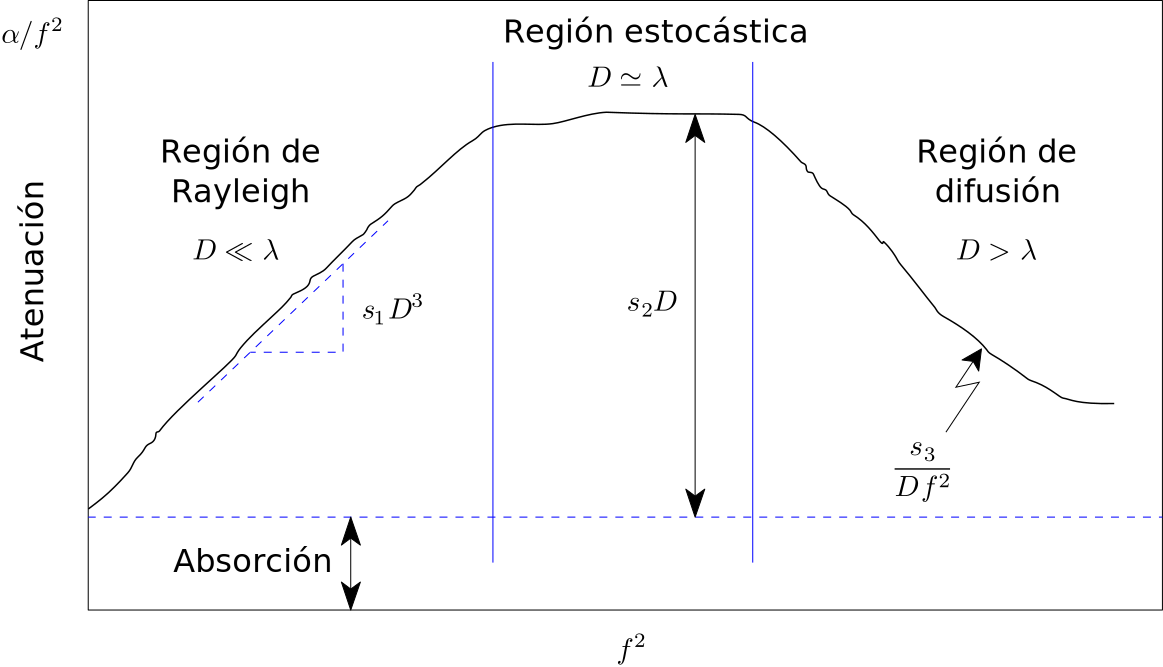
\includegraphics{gis-pfc-ch5-06.jpg}
	\end{center}
	\caption[Comportamiento del coeficiente de atenuación en las
	distintas regiones del medio]{Representación del coeficiente de
	atenuación que muestra su comportamiento en las distintas regiones
	del material.}
	\label{fig:losscoefficient}
\end{figure}

Para finalizar este apartado, en la \vref{fig:losscoefficient} se muestra
una representación del coeficiente de atenuación, en concreto del cociente
$\alpha/f^2$, con respecto al cuadrado de la frecuencia. En la gráfica es
posible apreciar el comportamiento del coeficiente de dispersión en cada
una de las regiones descritas, y como el término que introduce la absorción
es de valor constante con la frecuencia. La región de difusión muestra una
atenuación abrupta que responde a una exponencial decreciente descrita por
la expresión $s_3/(Df^2)$.


\subsection{Limitaciones impuestas por la dispersión en los ensayos
ultrasónicos}

La dispersión, que contribuye de dos modos distintos a perjudicar el
proceso de inspección ultrasónica, por un lado atenuando la señal acústica,
por otro lado causando el ruido de grano, es el principal factor limitante
en los ensayos no destructivos. Es habitual que la dispersión limite la
profundidad de una inspección a la región de Rayleigh.

Cualquier material posee granos de diferentes tamaños y, por tanto, un
frente de ondas acústicas que atraviesa un material se ve afectado por la
dispersión como si se encontrase en las tres regiones de dispersión
descritas. No obstante, es el grano de mayor tamaño el que en la práctica
determina el comportamiento del material en términos de dispersión.

La dispersión, debido a que es el causante del ruido estructural, no puede
contrarrestarse aumentando la potencia de la onda ultrasónica en emisión.
La solución primera para evitar la dispersión pasa por disminuir la
frecuencia de la onda, pero esto desemboca también en una pérdida de
resolución. La mejor alternativa consiste en emplear técnicas de
procesamiento de señal que reduzcan la energía del ruido estructural en
recepción.


\section{Algoritmos utilizados para la reducción del ruido estructural}

Dejando a un lado las técnicas empleadas en la eliminación de ruido
incoherente aleatorio, ineficaces por completo contra el ruido estructural,
existe un conjunto de métodos orientados a combatir este tipo de ruido.

Las técnicas empleadas con mayor frecuencia con el objeto de conseguir
mayor \sig{snr} en entornos en los que la presencia de ruido estructural es
notable son aquellas que aprovechan la diversidad de información hallada al
trabajar con señales incorreladas entre sí. Estas técnicas tratan de
obtener una señal con una mayor \sig{snr} a partir de la composición de
varias señales generadas mediante un mismo mecanismo pero de forma que la
medida de correlación entre cada una de ellas sea pobre. Los métodos
empleados más a menudo con tal propósito son:

\begin{itemize}
	\item Las técnicas que explotan la diversidad espacial, en las que
		básicamente se repite el mismo experimento variando cada
		vez la orientación de los transductores implicados en el
		mismo.
	\item Y las técnicas de diversidad frecuencial, manteniendo la
		posición de los transductores se repite el experimento
		utilizando señales situadas en una banda espectral
		diferente unas de otras.
\end{itemize}

Este tipo de técnicas consiguen mejorar de forma considerable la \sig{snr}
en inspecciones ultrasónicas, no obstante presentan una serie de
inconvenientes que las hacen inapropiadas en determinadas situaciones. Por
un lado, las técnicas de diversidad espacial se ven obstaculizadas con
frecuencia por las dimensiones y forma de las piezas evaluadas, siendo en
ocasiones imposible emplearlas. En cuanto a las técnicas de diversidad en
frecuencia, los transductores empleados en inspecciones ultrasónicas actúan
por lo común en una banda no lo bastante ancha como para poder dividirla en
un gran número de subbandas y así poder emitir suficientes señales
acústicas repartidas por el espectro de frecuencias. Para poder emplear una
técnica así serían necesarios varios transductores que emitiesen en bandas
de frecuencia señales acústicas con ancho de banda controlado y que todos
estuviesen situados en la misma posición.

La dificultad que conlleva implementar las técnicas anteriormente descritas
ha contribuido a la proliferación de técnicas que a partir de una única
traza sacan partido de las diferencias estadísticas que existen entre la
señal que procede de un defecto y el ruido estructural. Dentro de esta
categoría el algoritmo que ha alcanzado un éxito mayor y en consecuencia se
ha convertido en el paradigma de las técnicas de reducción de ruido
estructural se conoce como técnica de partición espectral o del inglés
\emph{Split Spectrum Processing} (\psig{ssp}) y fue en inicio propuesto por
Vernon Newhouse en 1982. El algoritmo está basado en la explotación de la
seudo"=diversidad frecuencial que existe entre las diferentes trazas de
banda estrecha que se obtienen al descomponer con un banco de filtros paso
banda la señal resultante tras un ensayo. No obstante los excelentes
resultados encontrados utilizando esta técnica, la gran sensibilidad que
muestra el algoritmo a la sintonía de los principales parámetros que
definen su comportamiento lo convierten en escasamente robusto. A
consecuencia de esto han aparecido numerosas publicaciones que se
circunscriben a proporcionar configuraciones del algoritmo que proporcionen
resultados óptimos, alternativamente aparecen también variaciones del
\sig{ssp} que persiguen mejorarlo. A pesar de su éxito, el \sig{ssp} no es
el único método empleado con el objetivo de sustraer el ruido de grano de
la señal de interés de un \sig{endus}. Otros trabajos incluyen, la
estimación de máxima verosimilitud, técnicas de filtrado paso"=banda que
eliminan la mitad superior del espectro de la señal, técnicas
tiempo"=frecuencia como son la transformada de Wigner"=Ville o las Wavelet,
técnicas que sacan partido de la información que aporta el retardo de
grupo, técnicas no lineales y, finalmente, técnicas de ruido residual.

A pesar del gran número de técnicas dedicadas a eliminar el ruido
estructural, son pocos los trabajos orientados a establecer una relación
entre ellas, a compararlas, a clasificarlas según su comportamiento en
distintos tipos de materiales o a justificar por qué el uso de una u otra
técnica.


\section{Técnicas de procesado por partición del espectro}

Bajo el término <<técnicas de procesado por partición del espectro>>, en
inglés \emph{Split Spectrum Processing Techniques}, o simplemente
\psig{ssp}, se reúnen una serie de algoritmos cuya aplicación es la
reducción del efecto del ruido estructural o de grano en los resultados de
un \sig{endus}. El principio en el que se fundamentan estas técnicas es
similar al que rige las técnicas de diversidad convencionales. A partir de
varias señales incorreladas entre sí se construye una señal cuya \sig{snr}
es considerablemente mejor que la \sig{snr} de cualquiera de las señales
primitivas por separado. Las técnicas de \sig{ssp}, a diferencia de las
técnicas basadas en la diversidad, consiguen sólo una seudo"=diversidad en
frecuencia a partir de una única traza de la señal que se obtiene tras un
\sig{endus}. Con frecuencia se obtienen buenos resultados empleando estas
técnicas lo que, sumado a la sencillez con la que puede implementarse un
experimento fundamentado en las mismas, recordando que no es requerida una
redundancia real basada en la utilización de varias señales, las ha
convertido en las técnicas más populares en el ámbito de los \sig{endus}. A
consecuencia de la reputación con la que se han visto revestidas
recientemente numerosas investigaciones se han llevado a cabo en las
décadas de los ochenta y los noventa, así como a principios de siglo, con
el fin de mejorar en la medida de lo posible los buenos resultados que ya
de por sí proporcionan las técnicas de \sig{ssp}.

El procedimiento (más detallado en el \cref{tab:sspfeatures}) que por lo
general sigue todo el conjunto de técnicas de \sig{ssp} consiste en aplicar
una transformación sobre la traza que comprende dos pasos:

\begin{itemize}
	\item El primero, dividir la traza en un número determinado de
		señales de banda estrecha, para lo que se emplea un banco
		de filtros.
	\item En segundo lugar se reconstruye la traza, o más bien una
		versión de ésta con una \sig{snr} mejorada, mediante un
		algoritmo de reconstrucción no lineal.
\end{itemize}

Las diferencias entre el carácter estadístico del ruido y de la señal
procedente del defecto hacen que el procedimiento anterior conduzca al
resultado deseado. Para concretar, la distribución de la energía del ruido
no es equitativa en frecuencia, de ahí que sea posible encontrar señales
incorreladas en ruido mediante la división espectral que realiza el banco
de filtros. Por otro lado, la linealidad que presenta la componente de la
señal ---o alteración de la misma según sea el caso--- originada en la
reflexión que se produce al encontrarse la onda acústica con el defecto
conlleva que la muestra que identifica la presencia del defecto se
encuentra en la misma posición en todas las trazas de banda estrecha. Los
métodos de \sig{ssp} aprovechan de manera implícita esta última
característica de la traza para magnificar la componente de la señal que
indica la presencia del defecto por lo que son catalogados en la
bibliografía como métodos que explotan la fase del defecto.


\begin{table}
	\centering
	\begin{tabulary}{.95\textwidth}{>{$(}c<{)$}Lr@{\hspace{6pt}}L}
		\toprule
		\multicolumn{2}{c}{Parámetros} %
		& \multicolumn{2}{c}{Algoritmo} \\
		\cmidrule(r){1-2}\cmidrule(l){3-4}
		y & Señal a procesar & 1. & Generar del banco de filtros \\
		f_\text{min} %
		& Frecuencia inferior de corte del banco de filtros & 2. %
		& Calcular la \sig{fft} de $y$ \\
		f_\text{max} %
		& Frecuencia superior de corte del banco de filtros & 3. %
		& Procesar el resultado obtenido en (2) con el banco de %
		filtros \\
		\Delta f & Separación entre filtros & 4. %
		& Calcular la \sig{ifft} de las trazas de banda estrecha \\
		pb & Ancho de banda de los filtros & 5. %
		& Normalizar la amplitud de las trazas de banda estrecha \\
		h_f & Tipo de filtro empleado & 6. %
		& Construir una única traza a partir de las trazas de %
		banda estrecha normalizadas \\
		\bottomrule
	\end{tabulary}
	\caption[Particularidades que en general se aplican a todos los
	algoritmos de \sig{ssp}]{Particularidades que en general se aplican
	a todos los algoritmos de \sig{ssp}.}
	\label{tab:sspfeatures}
\end{table}

\begin{figure}
	\begin{center}
		\includegraphics{gis-pfc-ch5-07.mps}
	\end{center}
	\caption[Parámetros de configuración del banco de filtros]%
	{Representación esquemática en la que pueden observarse los
	parámetros empleados en la configuración del banco de filtros
	comparados con el espectro de la señal de audio.}
	\label{fig:filter}
\end{figure}

La eficacia de las técnicas de \sig{ssp} no está garantizada, depende en
gran parte de dos de los parámetros listados en el \cref{tab:sspfeatures}.
Por un lado está la configuración del banco de filtros, a destacar dos
aspectos: el tipo de filtro empleado y la zona del aspecto en la que se
aplica el método. Según afirma M.\,A. Izquierdo (en \cite{garcia2000mrsr}),
trabajos realizados a principios de los noventa como los de P.\,Karpur
apuntan a la existencia de una relación entre el factor de forma de los
filtros que se utilizan para realizar la partición de espectro y la bondad
de los resultados aportados por la técnica de \sig{ssp}. Señala M.\,A.
Izquierdo que, a pesar de que la influencia que ejerce este parámetro en la
calidad del ensayo haya mostrado ser notable, estudios posteriores no han
tenido en cuenta las conclusiones alcanzadas por Karpur. La región del
espectro que queda bajo el banco de filtros puede configurarse ajustando
las frecuencias de corte superior e inferior del banco ---quedando
indirectamente condicionados el ancho de banda de los filtros y la
separación entre los mismos---. Es importante evitar que la banda de paso
del banco coincida con alguna porción de la señal en la que la información
espectral que indica la presencia del defecto quede enmascarada por el
ruido de grano. Cuando así ocurre la efectividad del método se reduce en
gran medida.

El parámetro que resta por considerar no es otro que el algoritmo de
reconstrucción que permite recuperar la traza definitiva. Las técnicas de
\sig{ssp} se basan en la estabilidad de la fase de ahí su precaria
robustez. El algoritmo de reconstrucción empleado es un factor determinante
del que depende en gran parte la robustez de la técnica. Por tanto, aplicar
un algoritmo de reconstrucción adecuado a las muestras es crucial para
obtener buenos resultados. Los algoritmos más empleados son el de mínimo
del ensamble y el del umbral de polaridad (\emph{Polarity Thresholding}) o
combinación de ambos, a continuación se citan otros.

Los trabajos mencionados en este apartado siguen todos una misma línea de
investigación, descubrir qué configuración del banco de filtros y qué
método de reconstrucción optimizan los resultados de aplicar las técnicas
de \sig{ssp} en un \sig{endus}. Se ha dicho que el término \sig{ssp} agrupa
a un conjunto de técnicas, lo que las diferencia precisamente es, o bien el
algoritmo de reconstrucción que emplean, o bien la forma en la que se
configura el banco de filtros, en ocasiones ambos. En cuanto a la
configuración del banco de filtros, algunos trabajos, es especial algunos
de Karpur, aportan avances significativos. El autor encuentra para el
algoritmo de mínimos, de forma analítica y apoyándose en un modelo
estacionario del ruido de grano, los parámetros que optimizan el
rendimiento de la técnica de \sig{ssp}. Los valores hallados son los
siguientes:

\begin{equation}
	\begin{split}
		N & = B\cdot T_y + 1 \\	
		b & = \Delta f = \frac{1}{T_y}
	\end{split}
\end{equation}

Donde $N$ representa el número óptimo de filtros, $B$ el ancho de banda del
transductor en el segmento de recepción, $T_y$ la duración de la señal
recibida, $b$ el ancho de banda de cada filtro, y $\Delta f$ la separación
entre filtros. Por otro lado Karpur afirma en otro de sus estudios, esta
vez apoyándose en la expresión para la atenuación en la región de Rayleigh,
que el banco de filtros debe aplicarse en las frecuencias más bajas del
espectro de la señal, ya que es en esa zona en la que se concentra la mayor
parte de la energía correspondiente a la radiación que tiene origen en el
defecto. Otros estudios utilizan la información relativa a la distribución
espectral de la \sig{snr}, obtenida mediante algoritmos como el del
histograma espectral o a partir de estadísticos del retardo de grupo como
p.e. la entropía móvil, para determinar cuál es la región del espectro de
la señal en la que es óptimo aplicar el filtrado.

En cuanto a los algoritmos de reconstrucción J.\,Saniie llega a la
conclusión, en su trabajo de 1991 en el que estudia los filtros de orden
aplicados como algoritmos de composición, de que los mejores resultados se
obtienen cuando la señal proviniente del defecto y el ruido estructural
están estadísticamente separados en un determinado cuantil. Dependiendo de
las distribuciones de probabilidad del ruido y del defecto, resulta
apropiado emplear algoritmos de mínimos, mediana o máximos del ensamble,
aunque por lo general el algoritmo de mínimos es el que mejores resultados
proporciona.

Por su parte M.\,G.\,Gustafsson propone una variante en el conjunto de las
técnicas de \sig{ssp} en la que, basándose en la teoría bayesiana de
detección y a partir de la información de la señal y el ruido coherente,
pueden encontrarse todos los parámetros necesarios para aplicar la técnica
de \sig{ssp}. El nombre que recibe usualmente esta variante es técnica de
\sig{ssp} con detección óptima.


\part*{Apéndices}

\appendix
\addtocounter{totalpages}{\value{page} + 1}
\pagenumbering{bychapter}
\chapter{Guía de usuario de la aplicación de control}\label{chap:appendixA}

\section{Instalación de los drivers y la aplicación}

Antes de poder utilizar la aplicación es preciso instalar correctamente en
el equipo la tarjeta de adquisición y los drivers de la tarjeta. Los
drivers pueden descargarse desde el sitio web del fabricante
(\url{http://www.keithley.com}).

Para poder utilizar la aplicación es necesario haber instalado previamente
en el \pc{} anfitrión una distribución de \matlab{} (revisión posterior a
2006a).

Para instalar la aplicación copiar el archivo \func{single\_channel.m} y el
archivo con extensión \func{single\_channel.fig} en el directorio de
trabajo.


\section{Especificaciones}

Para obtener información acerca de las prestaciones y limitaciones de la
aplicación véase el \vref{subsec:transducerconclusions}.


\section{Procedimientos de llamada}

Desde la ventana principal de \matlab{} es posible lanzar la aplicación de
tres modos diferentes.

\begin{itemize}
    \item En el navegador del sistema de archivos click derecho en el
	fichero \func{single\_channel.m}. Después seleccionar la opción
	<<ejecutar archivo>>.
    \item Ejecutar \sig{guide} (editor de interfaces gráficas de usuario).
	Abrir el fichero \func{single\_channel.fig}. Después click en el
	botón ejecutar de \sig{guide}.
    \item En el prompt de la ventana de comandos introducir el siguiente
	comando (cerciorarse previamente de que \matlab{} se encuentra en
	el directorio de trabajo).

	\begin{center}
	    \begin{lstlisting}[gobble=12]
		[handles = ]single_channel[(opciones)]
	    \end{lstlisting}
	\end{center}
\end{itemize}

El tercer procedimiento de llamada da acceso a las variables almacenadas en
el dominio interno de la aplicación como, por ejemplo: el búffer en el que se
almacenan las muestras recogidas o el objeto dispositivo que controla el
comportamiento de la tarjeta de adquisición.

La aplicación reutiliza cualquier objeto dispositivo asociado a la tarjeta
de adquisición, si no lo hubiera creo uno propio.


\section{Interfaz de usuario}

La \vref{fig:interface} muestra el aspecto de la interfaz gráfica de
usuario de la aplicación. La interfaz gráfica permite la interacción con el
sistema de medida, pueden encontrarse en ella 6 paneles.

\begin{figure}
    \begin{center}
	\includegraphics{gis-pfc-appa-01.png}
    \end{center}
    \caption[Aspecto de la interfaz de usuario]{Disposición de los
	distintos paneles de control y visualizadores en la interfaz de
	usuario.}
    \label{fig:interface}
\end{figure}

\begin{enumerate}
    \itembf{Panel de control principal} Alberga los controles que
	permiten configurar las propiedades básicas de la sesión de
	adquisición.
    \itembf{Panel de control secundario} Los mandos contenidos en
	este panel permiten controlar aspectos secundarios de la sesión de
	adquisición.
    \itembf{Visor} En el visor se muestran los resultados
	numéricos.
    \itembf{Ventana de representación grande} En esta ventana la
	representación ocupa un tamaño mayor.
    \itembf{Ventana de representación pequeña} En esta ventana la
	representación se hace a escala reducida.
    \itembf{Controles gráficos} Permiten habilitar o inhabilitar una o
	ambas representaciones gráficas.
\end{enumerate}


\subsection{Panel de control principal}

A continuación se enumeran los distintos botones y visualizadores que
integran el panel de control, su disposición en el panel se ilustra en la
\vref{fig:firstcontrolpanel}.

\begin{enumerate}
    \itembf{Selector de canal} Permite seleccionar el canal del que se
	extrae información. Sólo se puede seleccionar un canal a la vez.
    \itembf{Selector de frecuencia} Permite ajustar la frecuencia de
	muestreo de la tarjeta de adquisición. El valor de la frecuencia de
	muestreo debe estar contenido entre 1 kHz y la máxima frecuencia de
	muestreo permitida.
    \itembf{Control de ganancia} Ajusta la ganancia de amplificación del
	amplificador de instrumentación integrado en la tarjeta. Determina
	el rango máximo de la señal de entrada.
    \itembf{Indicador de rango} Rango máximo en el que debe estar contenida
	la señal de entrada (si la señal excede este rango tras ser
	amplificada internamente satura el conversor \sig{a/d} de la
	tarjeta de adquisición).
    \itembf{Control \sig{u/b}} Controla el modo de adquisición
	(unipolar/bipolar).
    \itembf{Control d/s} Controla el modo de terminación
	(diferencial/sencillo). Altera el comportamiento del selector de
	canal (lista 8 canales en modo diferencial y 16 en modo sencillo).
    \itembf{Control de on/off} Inicia o detiene respectivamente la sesión
	de adquisición.
\end{enumerate}


\subsection{Panel de control secundario}

Los elementos contenidos en el panel de control secundario son los listados
a continuación. La \cref{fig:secondcontrolpanel} muestra su ubicación
relativa en el panel.

\begin{enumerate}
    \itembf{Selector de tipo de medida} Permite seleccionar el tipo de
	resultado devuelto: muestra individual, media aritmética o
	representación gráfica de la señal y su espectro en frecuencia.
    \itembf{Ventana \sig{fft}} Permite seleccionar el número de puntos con
	el que se realiza la \sig{fft} utilizada para representar el
	espectro de la señal.
    \itembf{División temporal} Controla la duración del fragmento de señal
	representado gráficamente. Activa o desactiva el modo de
	representación continuo.
    \itembf{Cambio de ventana} Intercambia la ventana (ventanas de
	representación grande y pequeña) en la que se representan
	gráficamente la señal y su espectro en frecuencia.
\end{enumerate}

\newlength{\biggestpanel}
\settoheight{\biggestpanel}{\includegraphics{gis-pfc-appa-02.png}}

\begin{figure}
    \begin{center}
	\subfloat[Elementos del panel de control principal][Panel de
	    control principal.]{
	    \label{fig:firstcontrolpanel}
	    \begin{minipage}[top][\biggestpanel][c]{.425\textwidth}
		\centering
		\includegraphics{gis-pfc-appa-02.png}
	    \end{minipage}}
	\subfloat[Elementos del panel de control secundario][Panel de
	    control secundario.]{ \label{fig:secondcontrolpanel}
	    \begin{minipage}[top][\biggestpanel][c]{.425\textwidth}
		\centering
		\includegraphics{gis-pfc-appa-03.png}
	    \end{minipage}}
    \end{center}
    \caption[Paneles de control de la interfaz de usuario]{Esta figura
    muestra los distintos elementos que integran los paneles de control
    principal y secundario de la interfaz de usuario.}
    \label{fig:controlpanels}
\end{figure}

\subsection{Visor}

En el visor se pueden observar los resultados que proporcionan los modos de
funcionamiento numéricos. Los resultados se dan con una precisión de
decenas de milivoltios.


\subsection{Ventanas de representación grande y
pequeña}\label{subsec:windows}

Las representaciones se realizan en estas dos ventanas, cada ventana
alberga simultáneamente una única representación. El control de cambio de
ventana permite intercambiar la ventana en la que se representan señal y
espectro en frecuencias, por defecto la señal se representa en la ventana
grande y su espectro frecuencial en la ventan pequeña. Al pulsar el botón
cambio de ventana se intercambian también las marcas de gráfico, el título
y la rejilla. Los controles situados en el margen de cada ventan duplican o
dividen por dos la escala de amplitud de la representación.

\subsection{Controles gráficos}\label{subsec:gfoptions}

Los controles de este panel gráfico habilitan o inhabilitan la
representación gráfica de la señal y de su espectro en frecuencia
respectivamente. No tienen ninguna función en los modos numéricos de
funcionamiento.


\section{Inicio y detención de la sesión de adquisición}

El control on del panel principal de la interfaz de usuario inicia la
sesión de adquisición. Por su parte el control off detiene el muestreo. Al
pulsar en el control on se inhabilitan todos los controles de la interfaz
de usuario exceptuando los siguientes: control off, ventana \sig{fft},
cambio de ventana, controles de las ventanas de representación y controles
del panel opciones gráficas. Al pulsar off todos los controles
inhabilitados se restablecen.


\section{Modos de funcionamiento}

Existen tres modos de funcionamiento: muestra individual, media aritmética
y representación gráfica. Cada uno de ellos aporta distintos resultados.


\subsection{Muestra individual}

En este modo el visor muestra el valor de la última muestra adquirida (la
frecuencia de adquisición es de 4 Hz).

Si la señal evaluada oscila a una frecuencia elevada los valores observados
cambian rápidamente por lo que no resultan nada útiles.


\subsection{Media aritmética}

En este modo el visor muestra la media aritmética de las muestras
adquiridas en un espacio de tiempo de 250 ms. El número de muestras
utilizado para realizar la media depende de la frecuencia de muestreo (la
frecuencia de adquisición puede ajustarse mediante el selector de
frecuencia).

El visor se refresca cada 250 ms cuando este modo está activado. Si la
señal estudiada oscila rápidamente en el visor puede observarse el valor
<<$0.00$>>.


\subsection{Representación gráfica}

En este modo de funcionamiento se muestra el aspecto de la señal y el de su
espectro en frecuencias. Al seleccionar el modo de funcionamiento gráfico
se inhabilita el selector de frecuencia y se fija la frecuencia de muestreo
a la máxima frecuencia de muestreo posible (100 kHz si no se han añadido
más canales al objeto dispositivo asociado a la tarjeta).

Según la configuración de control división temporal se utiliza uno de los
dos modos de representación implementados.


\subsubsection{Modo de representación disparado}

La representación de la señal se muestra fija en el centro de la ventana de
representación. Este modo es útil para observar señales que oscilan a
frecuencias por encima de los 4 Hz, el disparo falla cuando se observan
señales que oscilan a una frecuencia inferior. Permite determinar
fácilmente la amplitud y la frecuencia de oscilación de la señal.


\subsubsection{Modo de representación continuo}

Este modo de representación se activa cuando la escala temporal de la
representación (control división temporal) se ajusta por encima de los 4
ms. En este modo la representación de la señal se desplaza de derecha a
izquierda a medida que avanza el tiempo. Este modo de representación es
útil para observar la forma de señales que oscilan a frecuencias inferiores
a los 4 Hz. También puede ayudar a determinar la amplitud de una señal. Sin
embargo es difícil averiguar la frecuencia a la que oscila una señal
observando la representación obtenida al activar este modo.


\section{Salida y limpieza}

Al cerrar la aplicación se detiene el proceso de muestreo y se elimina
último canal asignado al objeto dispositivo (si antes no se ha eliminado
ningún canal).

Al terminar la aplicación es necesario eliminar el objeto dispositivo y
limpiar el área de trabajo de \matlab{}.

\begin{center}
    \begin{lstlisting}
	aux = daqfind
	delete(aux);
	clear aux;
    \end{lstlisting}
\end{center}

\addtocounter{totalpages}{\value{page} - 1}
\chapter{Pruebas y contenidos adicionales}

Este apéndice no debe adjuntarse en el documento final, en el se anotarán
ideas para modificar el contenido del grueso del documento y bases para
generar los contenidos adicionales.


\section{Configuración de página}

La configuración actual se ha hecho utilizando el paquete \textsf{typearea}
que forma parte del conjunto del \textsc{koma}-\textsc{s}cript. Las
opciones más importantes que deben pasarse a este paquete son el tipo de
papel (A4, A3, A5, letter,\dots) y el espacio de corrección necesario para
evitar fallos en la encuadernación (\textsc{bcor} = \texttt{magnitud} o
directamente \textsc{bcor}\texttt{magnitud}). Utilizando el paquete
\textsf{layouts} pueden crearse figuras que representen la configuración de
página actual.

\newlength{\auxmm}
\newlength{\auxin}
\newlength{\auxpt}
\setlength{\auxmm}{1mm}
\setlength{\auxin}{1in}
\setlength{\auxpt}{1pt}
\newsavebox\caja
\sbox\caja{\includegraphics{gis-pfc-ch2-02.mps}}

\begin{table}
	\centering
	\printinunitsof{mm}\pagevalues\medskip\par

	\begin{tabular}{l l}
		\toprule
		1in = \printinunitsof{mm}\prntlen{\auxin} %
		& 1pt = \printinunitsof{mm}\prntlen{\auxpt} \\
		1mm = \printinunitsof{in}\prntlen{\auxmm} %
		& 1mm = \printinunitsof{pt}\prntlen{\auxmm} \\
		Alto de \texttt{gis-ch2-02.mps} %
		& \printinunitsof{mm}\prntlen{\ht\caja} \\
		Ancho de \texttt{gis-ch2-02.mps} %
		& \printinunitsof{mm}\prntlen{\wd\caja} \\
		marginparwidth %
		= \printinunitsof{pt}\prntlen{\marginparwidth} %
		& marginparsep %
		= \printinunitsof{pt}\prntlen{\marginparsep} \\
		\bottomrule
	\end{tabular}
	\caption[Valores actuales de la distribución de página]{Valores que
	completan el diagrama representado en la \vref{fig:layouts}
	sustituir la nomenclatura de referencia por los valores
	correspondientes}
\end{table}

\begin{figure}
	\begin{center}
		\includegraphics{gis-pfc-ch2-02.mps}
	\end{center}
	\caption[Segunda figura del segundo capítulo]{Segunda figura del
	segundo capítulo.}
	\label{fig:ch102}
\end{figure}

El lector puede fijarse que se cumple la regla de construcción que aplica
el paquete \textsf{typearea} en la que el margen inferior es dos veces el
margen inferior, y que el margen interior de página ---una vez eliminado el
centímetro (\textsc{bcor}\texttt{1cm}) que se deja para compensar el
encuadernado--- es la mitad del margen exterior de página. De ese modo se
crea una distribución de página en la que el margen interior de página de
las páginas par e impar juntas es igual a cada uno de los márgenes
exteriores de ambas páginas.

\begin{figure}
	\pagediagram
	\caption{Distribución del texto en las páginas de este documento}
	\label{fig:layouts}
\end{figure}

\begin{figure}\ContinuedFloat
	\currentpage
	\pagedesign
	\caption[]{Continuación del \vref{fig:layouts}}
\end{figure}


\section{Gráficos con MetaPost}

Anotaciones destinadas a obtener gráficos escalables de calidad empleando
el paquete MetaPost para la creación de gráficos en PostScript.


\subsection{Tamaño}

Tengo que modificar el tamaño de algunas figuras al haber cambiado la
tipografía predeterminada de la \emph{Computer Roman} a \emph{Lucida}. Lo
que quiero que aparezca en este apartado es un cuadro con los distintos
tamaños de letra que aparecen en el documento.


\backmatter

\addtocounter{totalpages}{\value{page} - 1}
\pagenumbering{arabic}
\setcounter{page}{\value{totalpages}}
\nocite{mittelbach2004lc, stutzman1997atd, garcia2000mrsr, pallas2004sas}
\bibliographystyle{bababbrv-lf}
\bibliography{gis-pfc}

\end{document}
